\section{Reconstruction error cuts for 2 leptons + $e_T^{miss}$}

In this section the remainding two reconstruction error cuts in the 2 lepton + $e_T^{miss}$ are shown. 
The figures here are shaped with the same subfigure structure as the figures in the results and 
discussion section. 
\subsection*{Regular autoencoder output}



\begin{figure}[H]
    \centering
    \begin{subfigure}{.40\textwidth}
        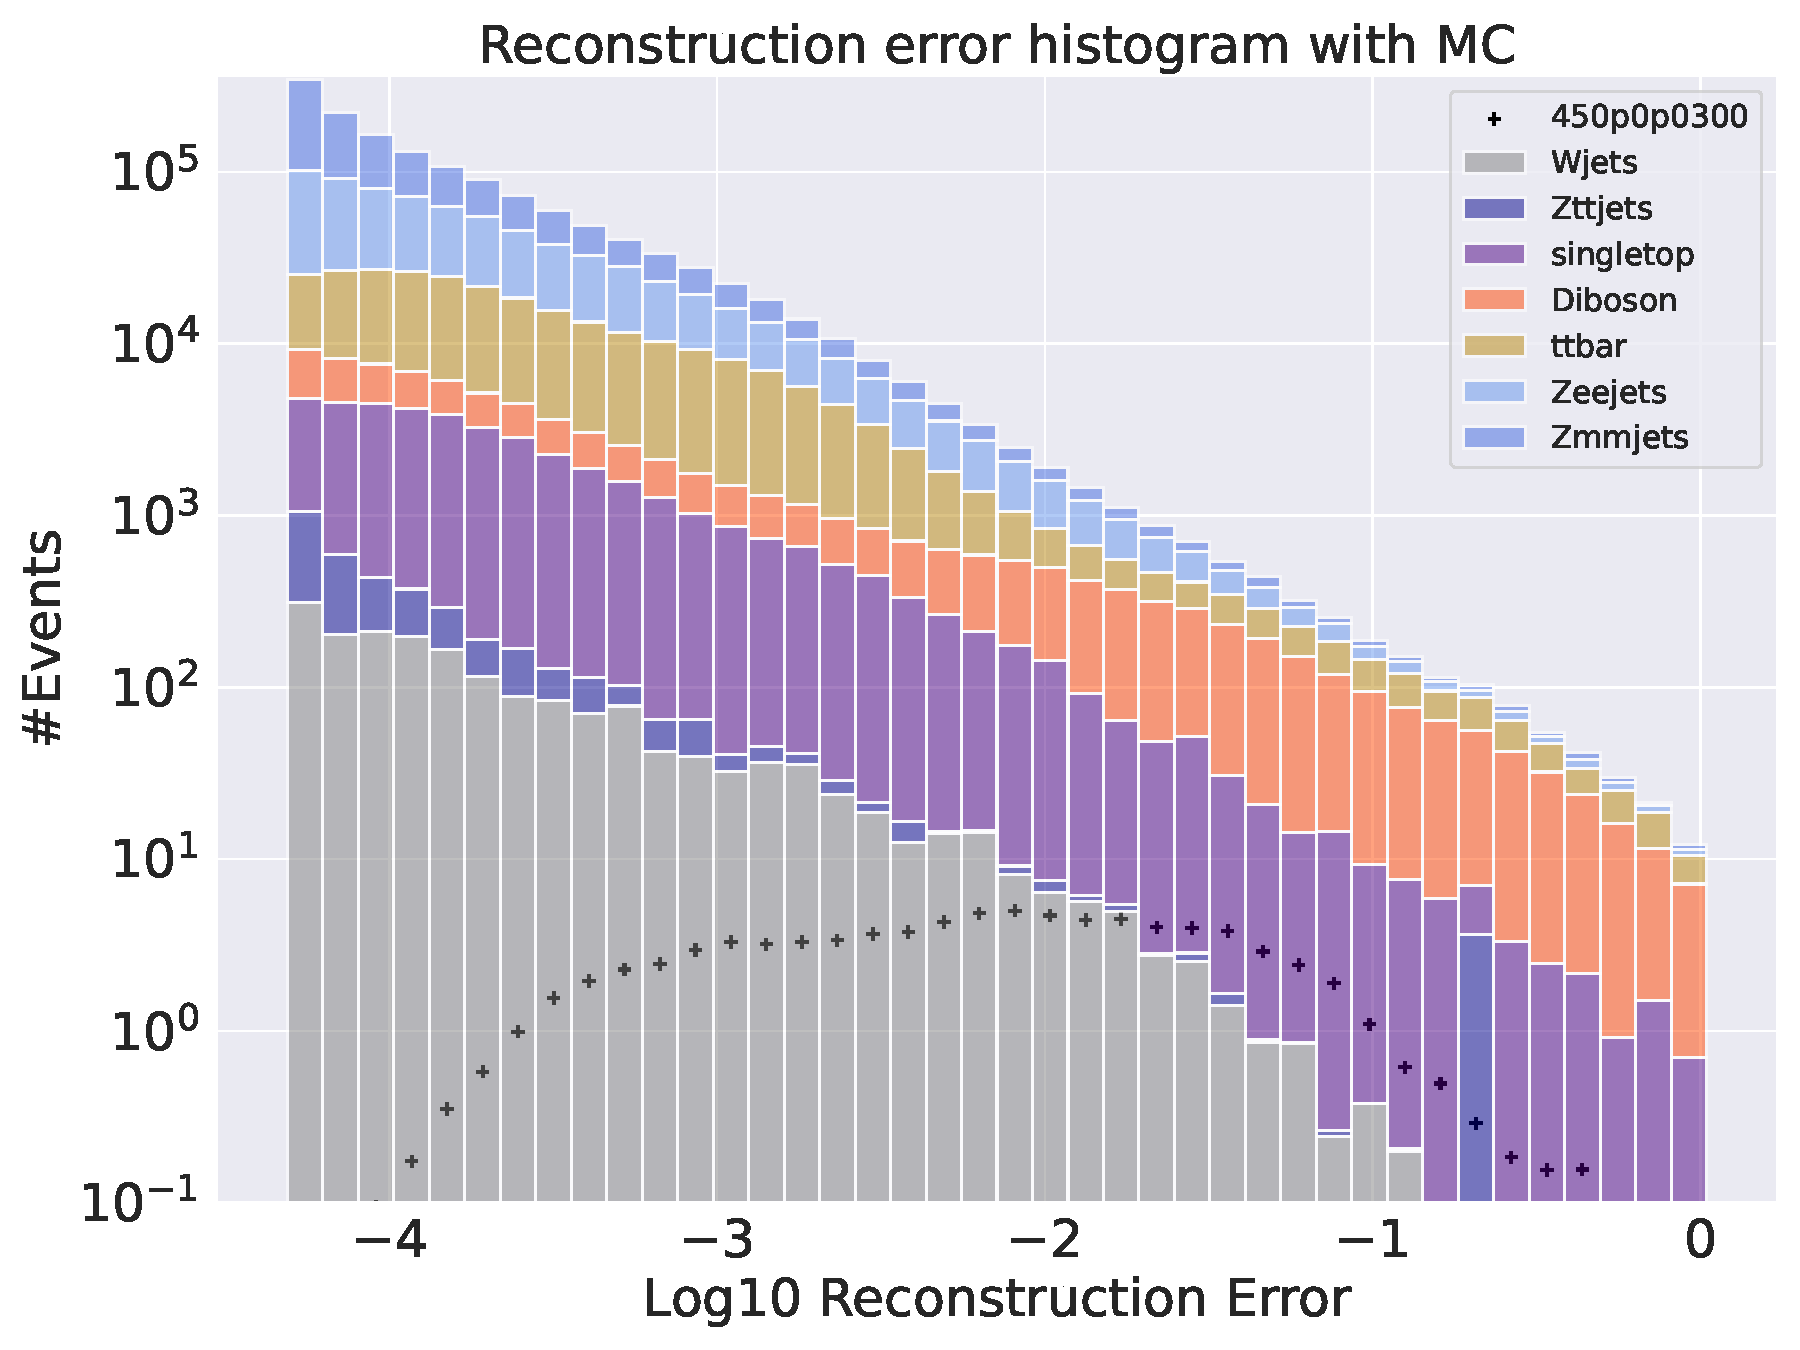
\includegraphics[width=\textwidth]{Figures/AE_testing/small/2lep/b_data_recon_big_rm3_feats_sig_450p0p0300_.pdf}
        \caption{ }
        \label{fig:AE_2lep_big_450_2}
    \end{subfigure}
    \hfill
    \begin{subfigure}{.40\textwidth}
        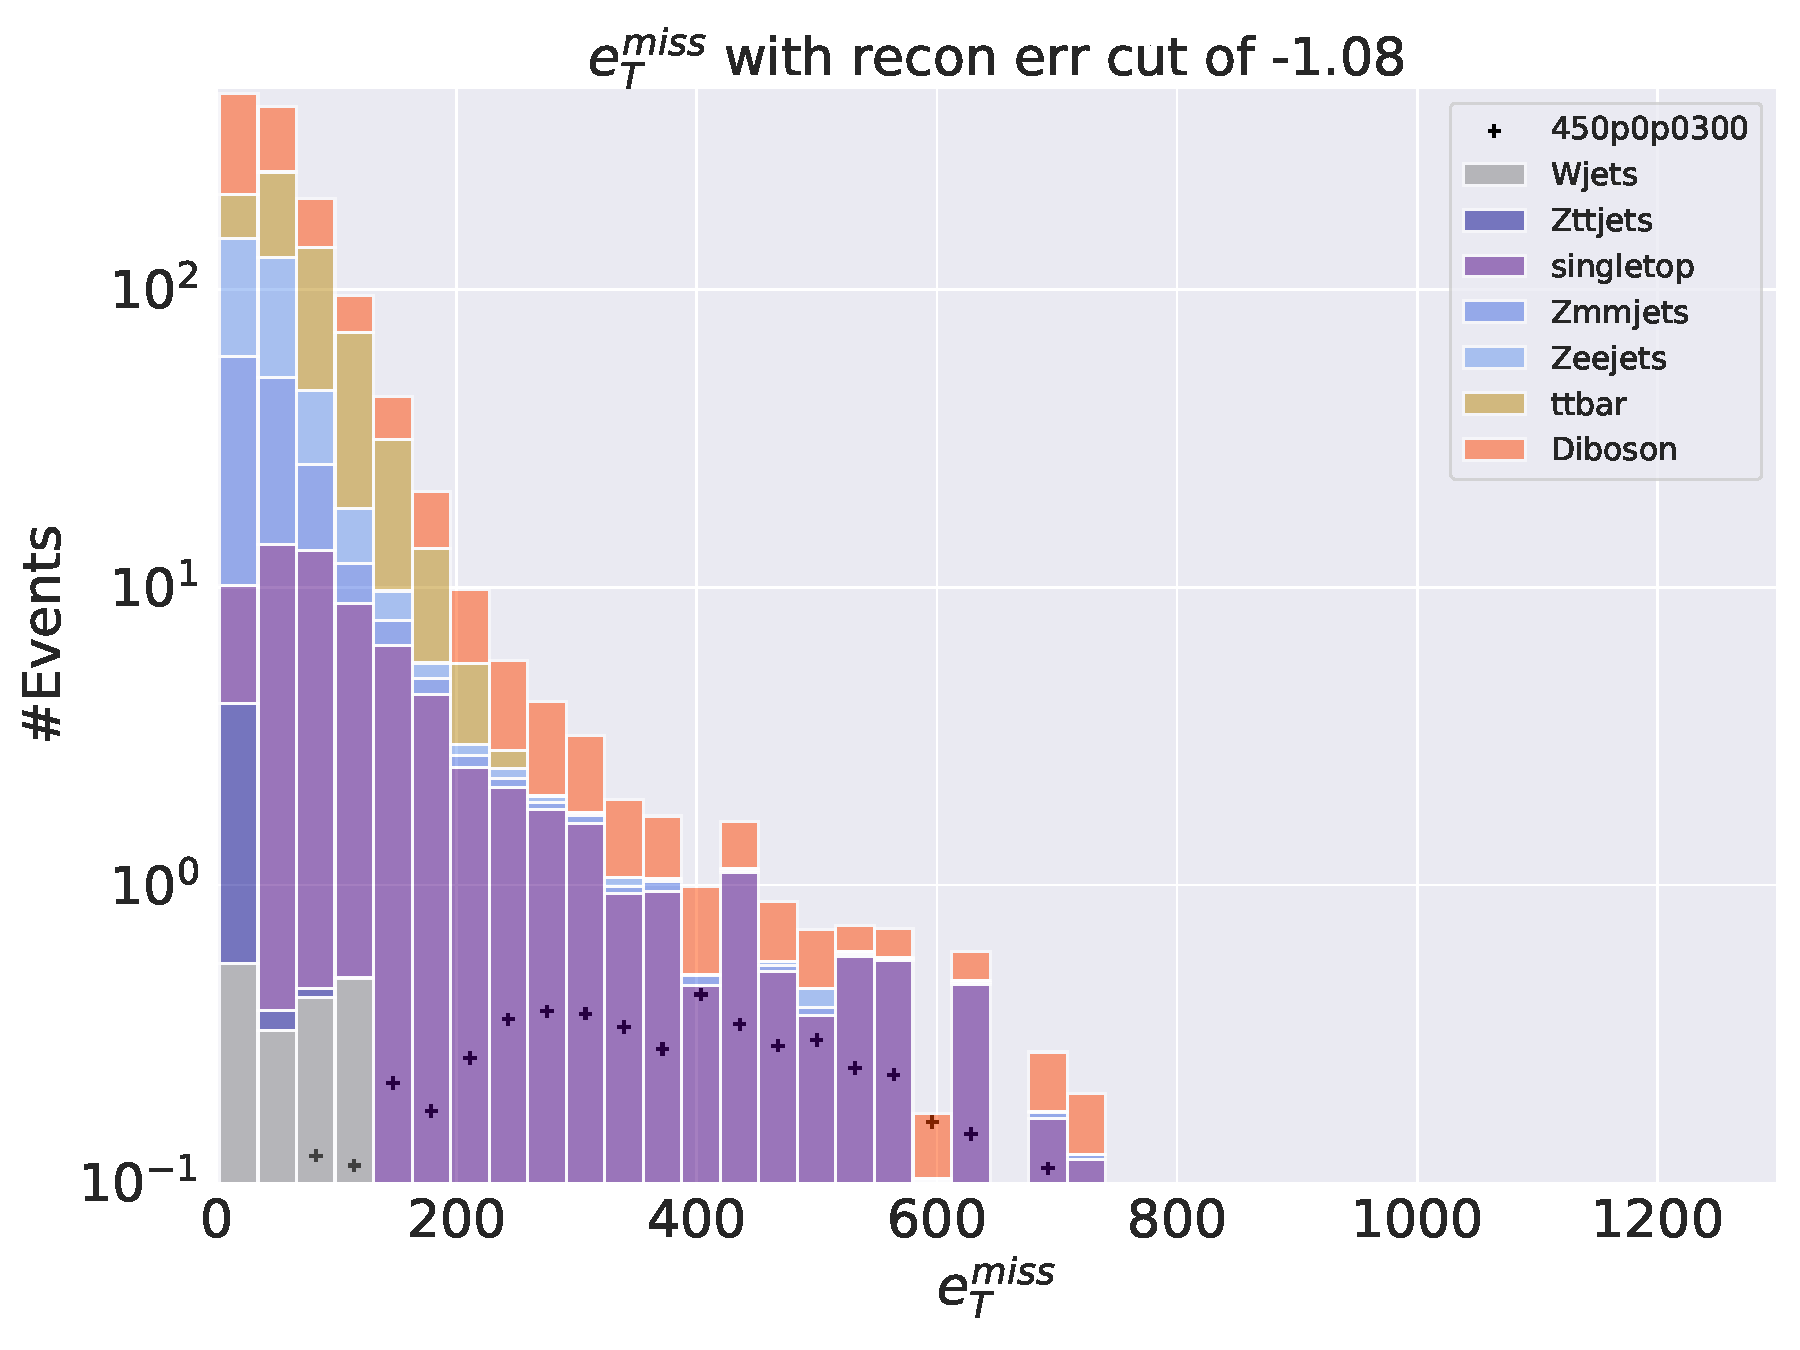
\includegraphics[width=\textwidth]{Figures/AE_testing/big/2lep/b_data_recon_big_rm3_feats_sig_450p0p0300_recon_errcut_-1.08.pdf}
        \caption{}
        \label{fig:AE_2lep_big_etmiss_450_2}
    \end{subfigure}
    \hfill 
    \begin{subfigure}{.40\textwidth}
        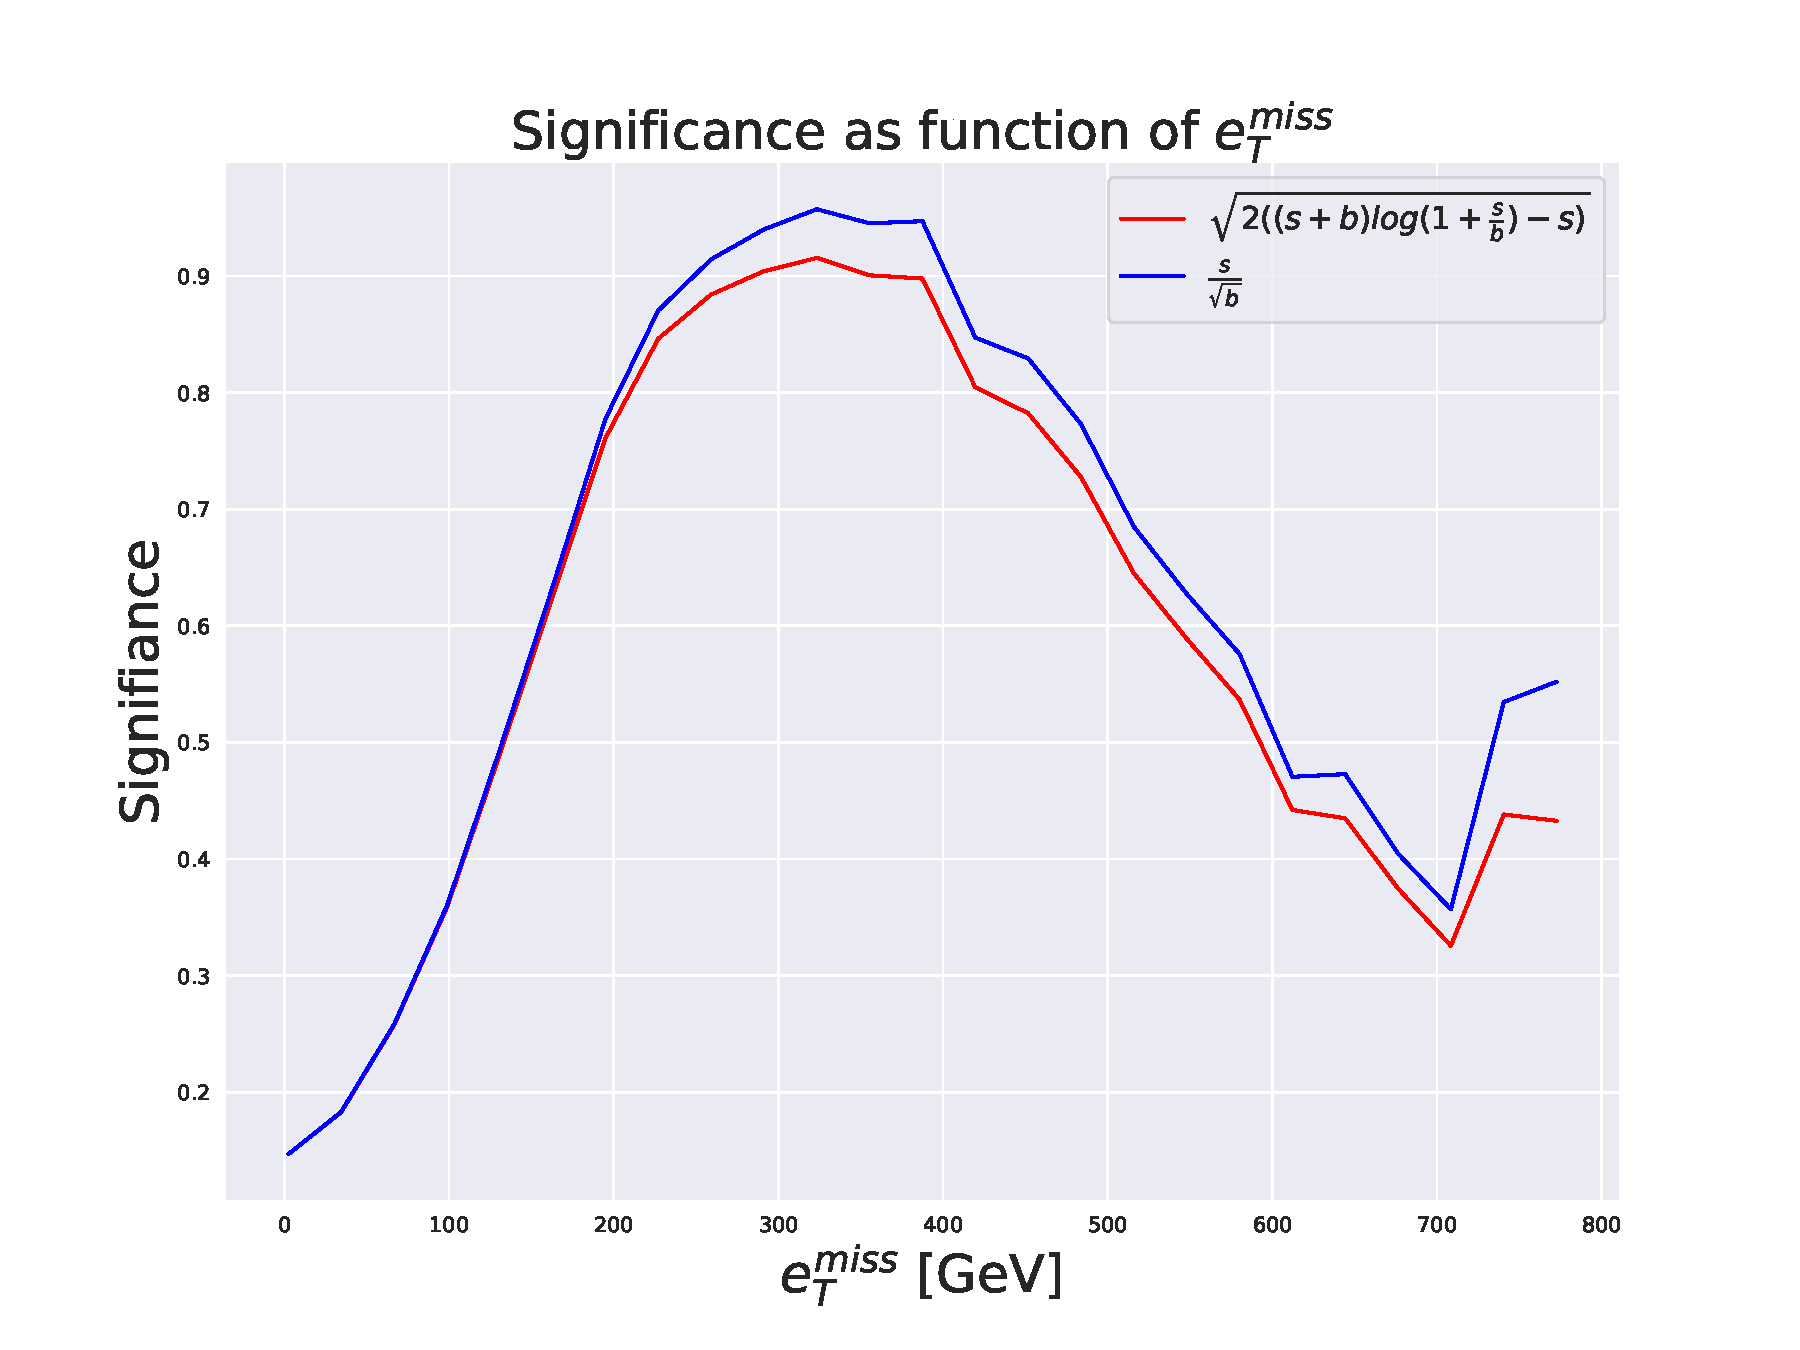
\includegraphics[width=\textwidth]{Figures/AE_testing/big/2lep/significance_etmiss_450p0p0300_-1.0770415453595523.pdf}
        \caption{}
        \label{fig:AE_2lep_big_signi_450_2}
    \end{subfigure}
    \hfill      
    \caption[2lep deep network | $450p300$ | AE | 2]{Reconstruction error, $e_T^{miss}$ signal region, $m_{lll}$ signal region and significance as function of 
    $e_T^{miss}$ for the deep regular autoencoder. Here the SUSY $450p300$ model is used.}
    \label{fig:AE_2lep_big_rec_sig_signi_450_2}
\end{figure}

\begin{figure}[H]
    \centering
    \begin{subfigure}{.40\textwidth}
        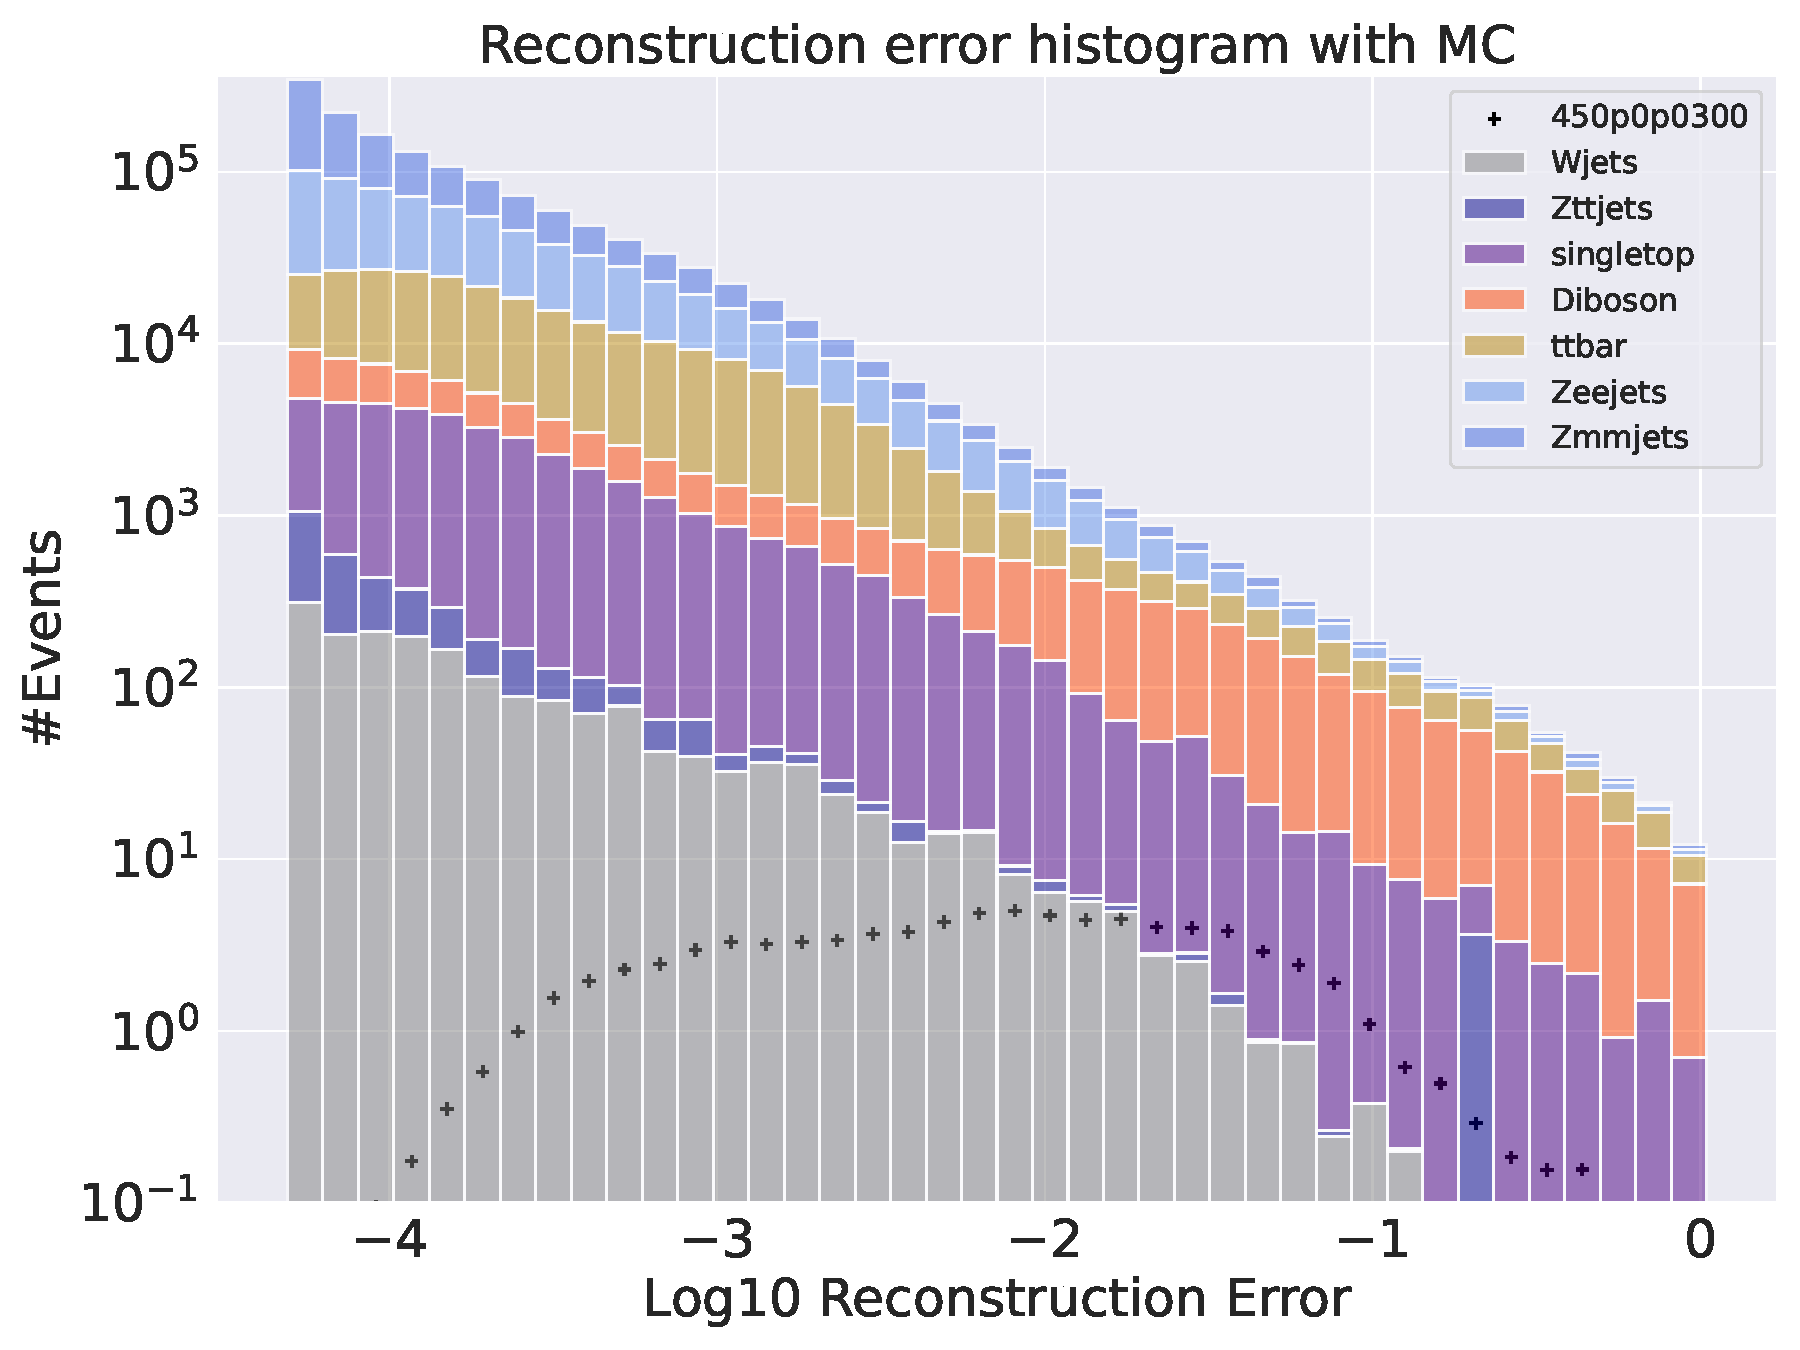
\includegraphics[width=\textwidth]{Figures/AE_testing/small/2lep/b_data_recon_big_rm3_feats_sig_450p0p0300_.pdf}
        \caption{ }
        \label{fig:AE_2lep_small_450_2}
    \end{subfigure}
    \hfill
    \begin{subfigure}{.40\textwidth}
        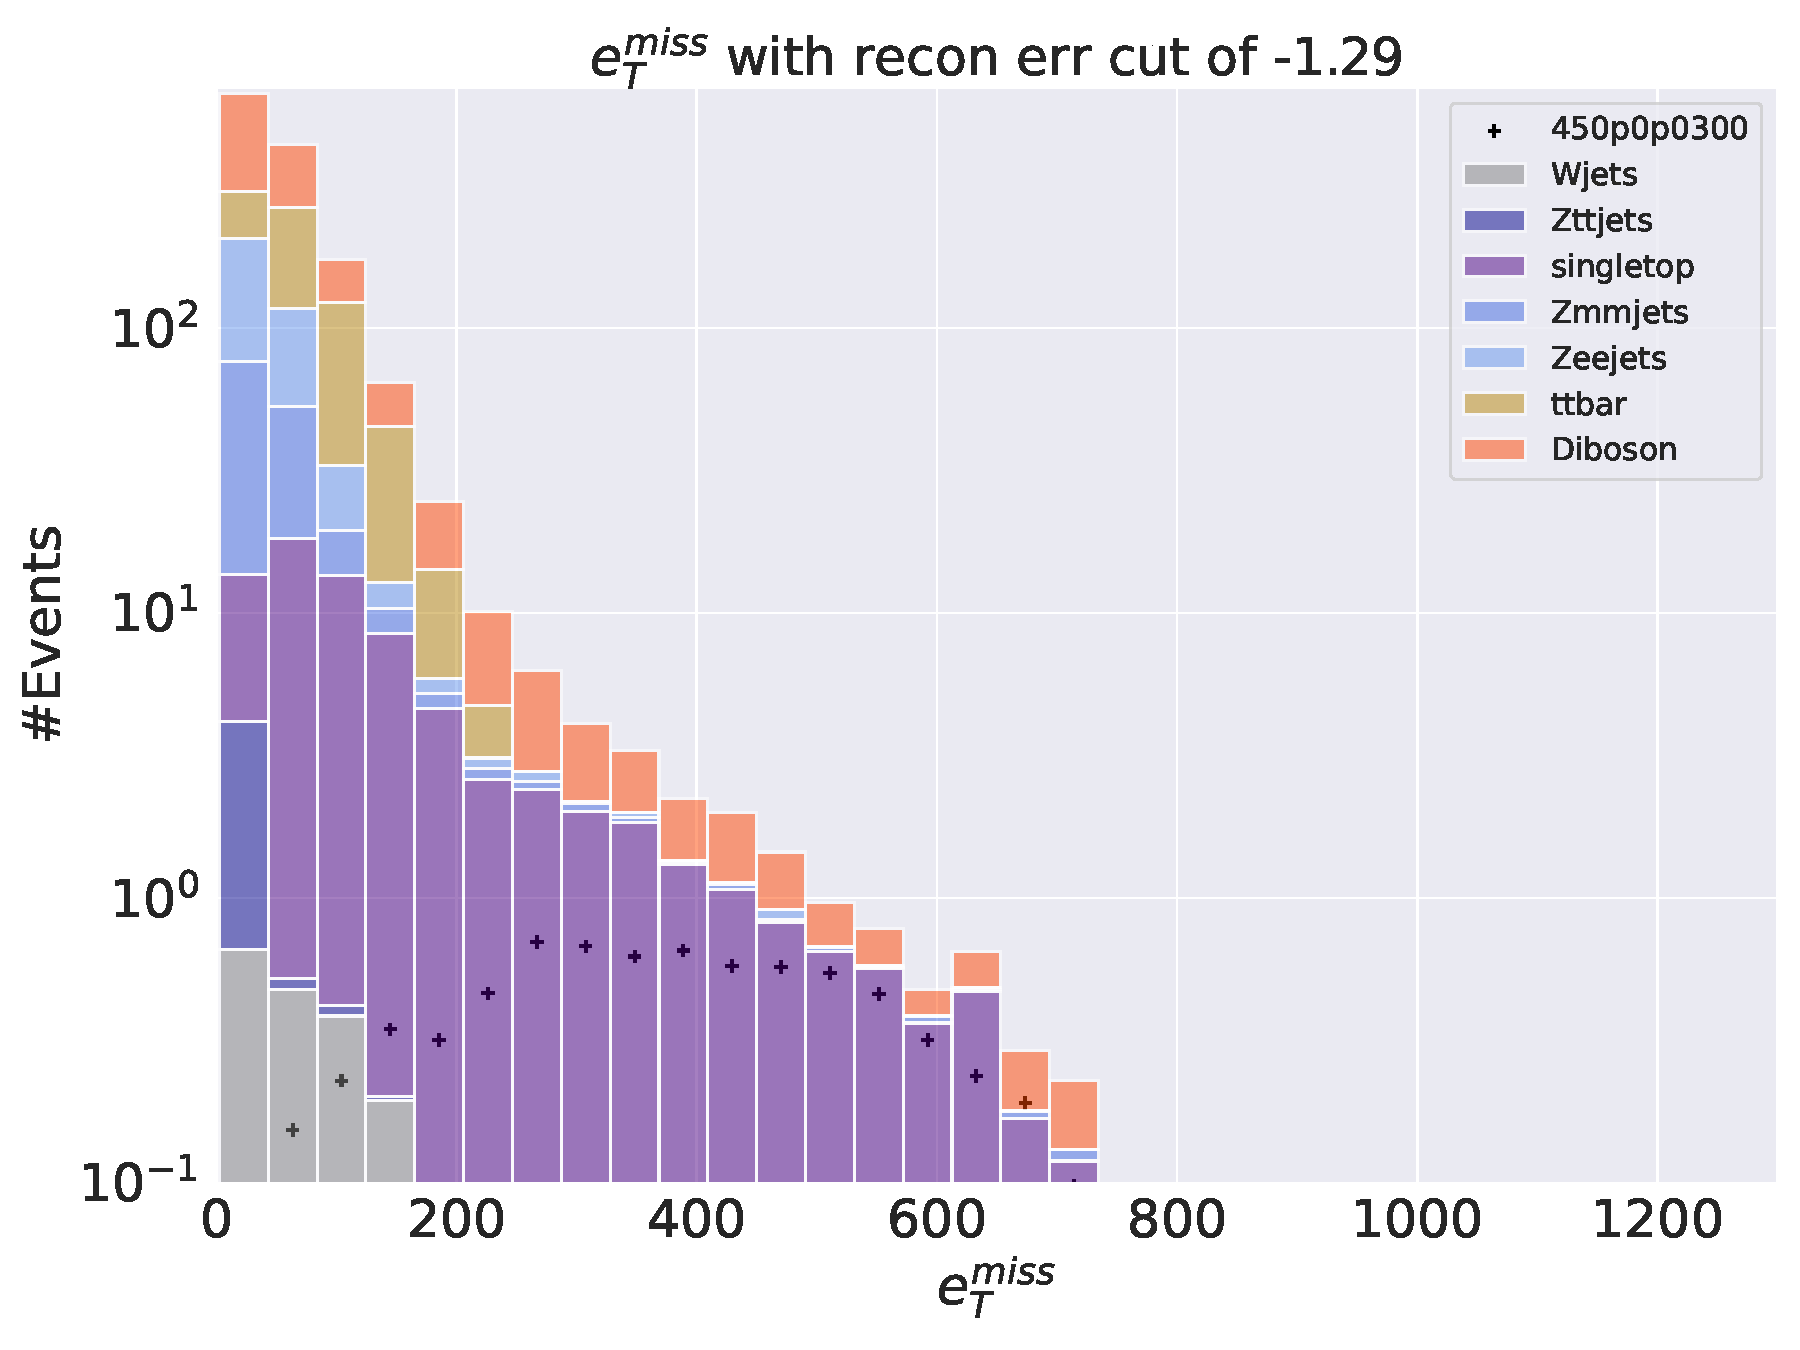
\includegraphics[width=\textwidth]{Figures/AE_testing/small/2lep/b_data_recon_big_rm3_feats_sig_450p0p0300_recon_errcut_-1.29.pdf}
        \caption{}
        \label{fig:AE_2lep_small_etmiss_450_2}
    \end{subfigure}
    \hfill  
    \begin{subfigure}{.40\textwidth}
        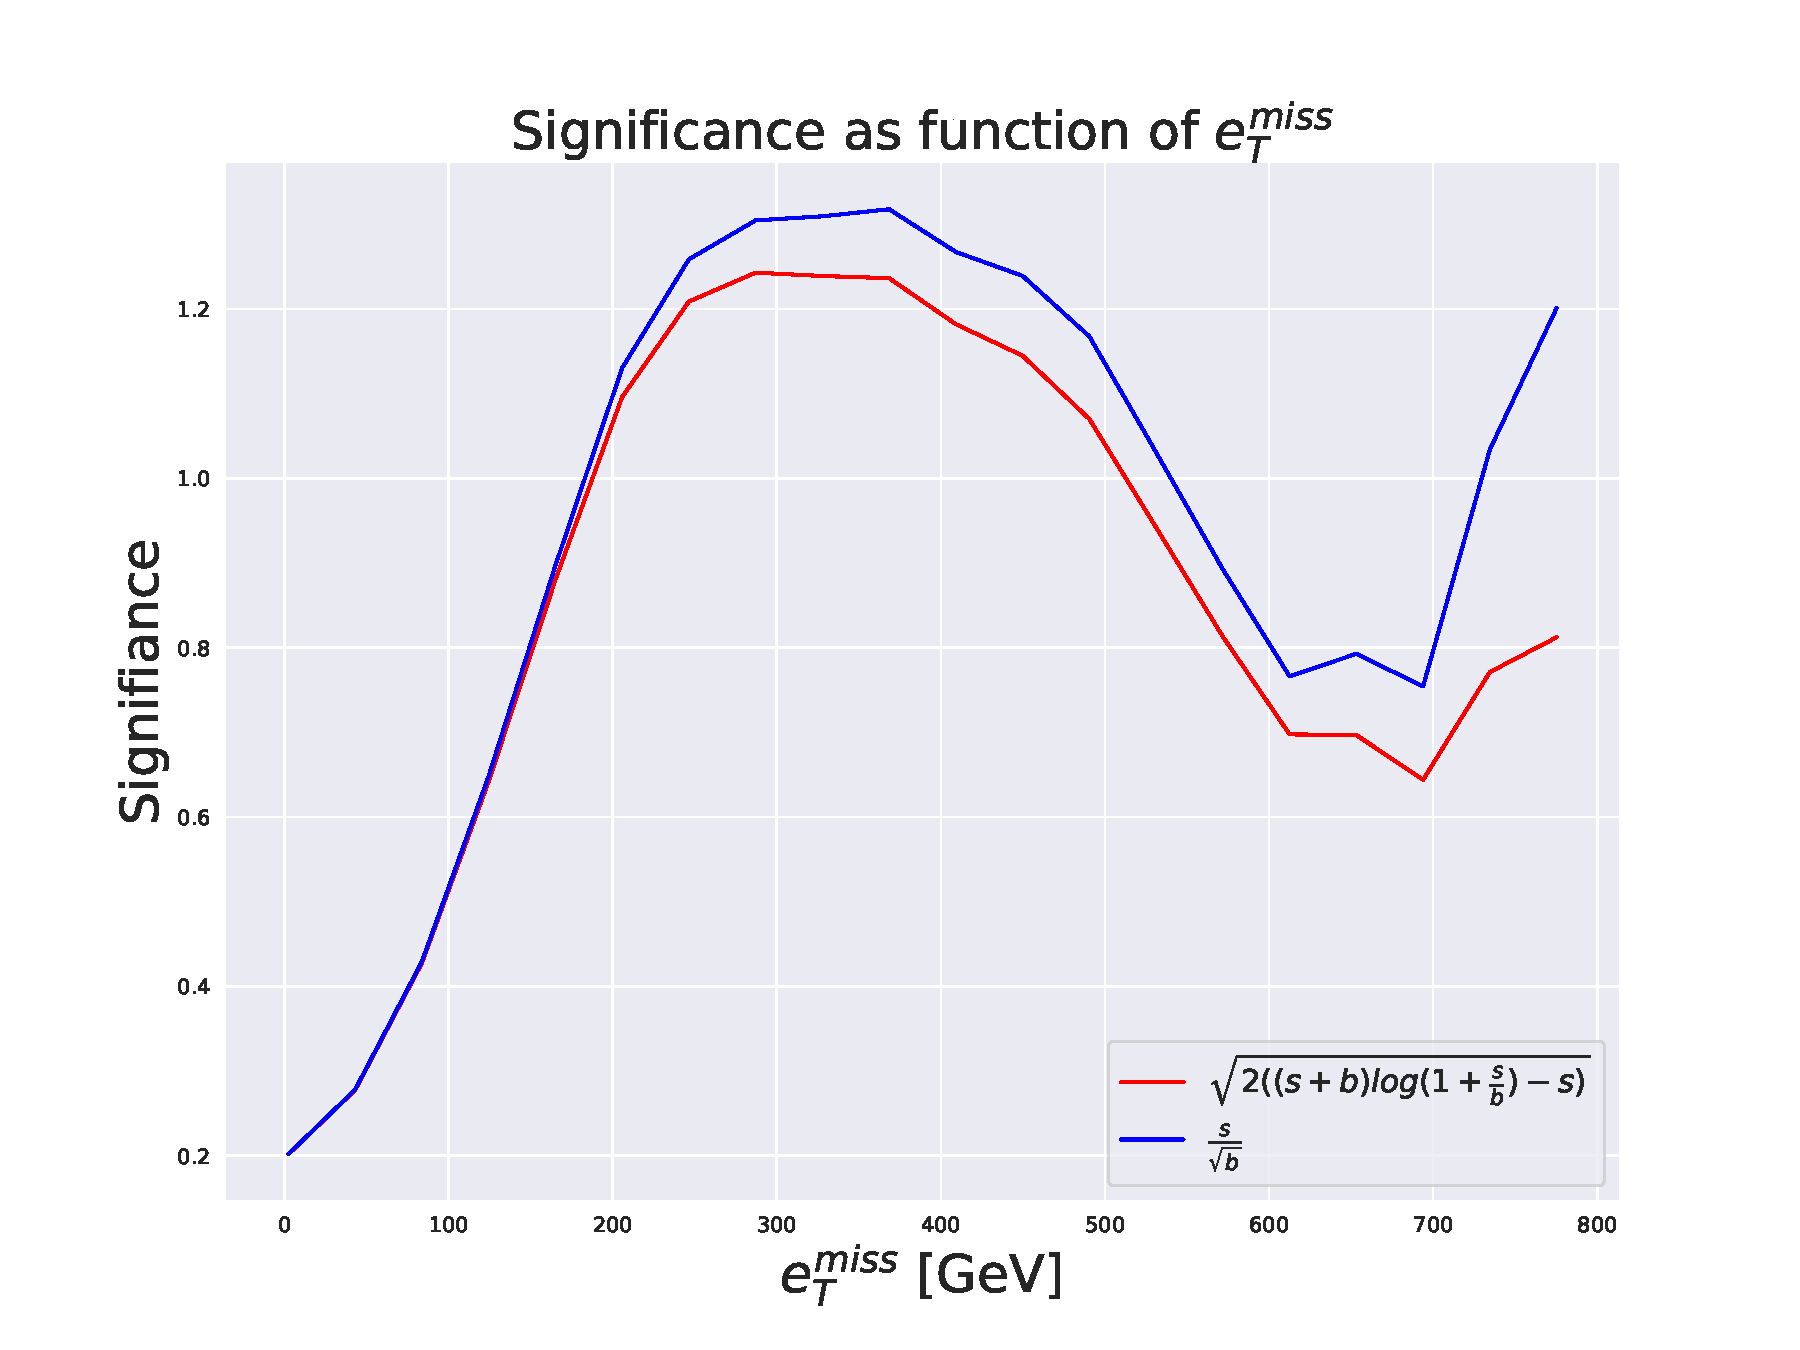
\includegraphics[width=\textwidth]{Figures/AE_testing/small/2lep/significance_etmiss_450p0p0300_-1.287562990021105.pdf}
        \caption{}
        \label{fig:AE_2lep_small_signi_450_2}
    \end{subfigure}
    \hfill      
    \caption[2lep shallow network | $450p300$ | AE | 2]{Reconstruction error, $e_T^{miss}$ signal region, $m_{lll}$ signal region and significance as function of 
    $e_T^{miss}$ for the deep regular autoencoder. Here the SUSY $450p300$ model is used.}
    \label{fig:AE_2lep_small_rec_sig_signi_450_2}
\end{figure}


\begin{figure}[H]
    \centering
    \begin{subfigure}{.40\textwidth}
        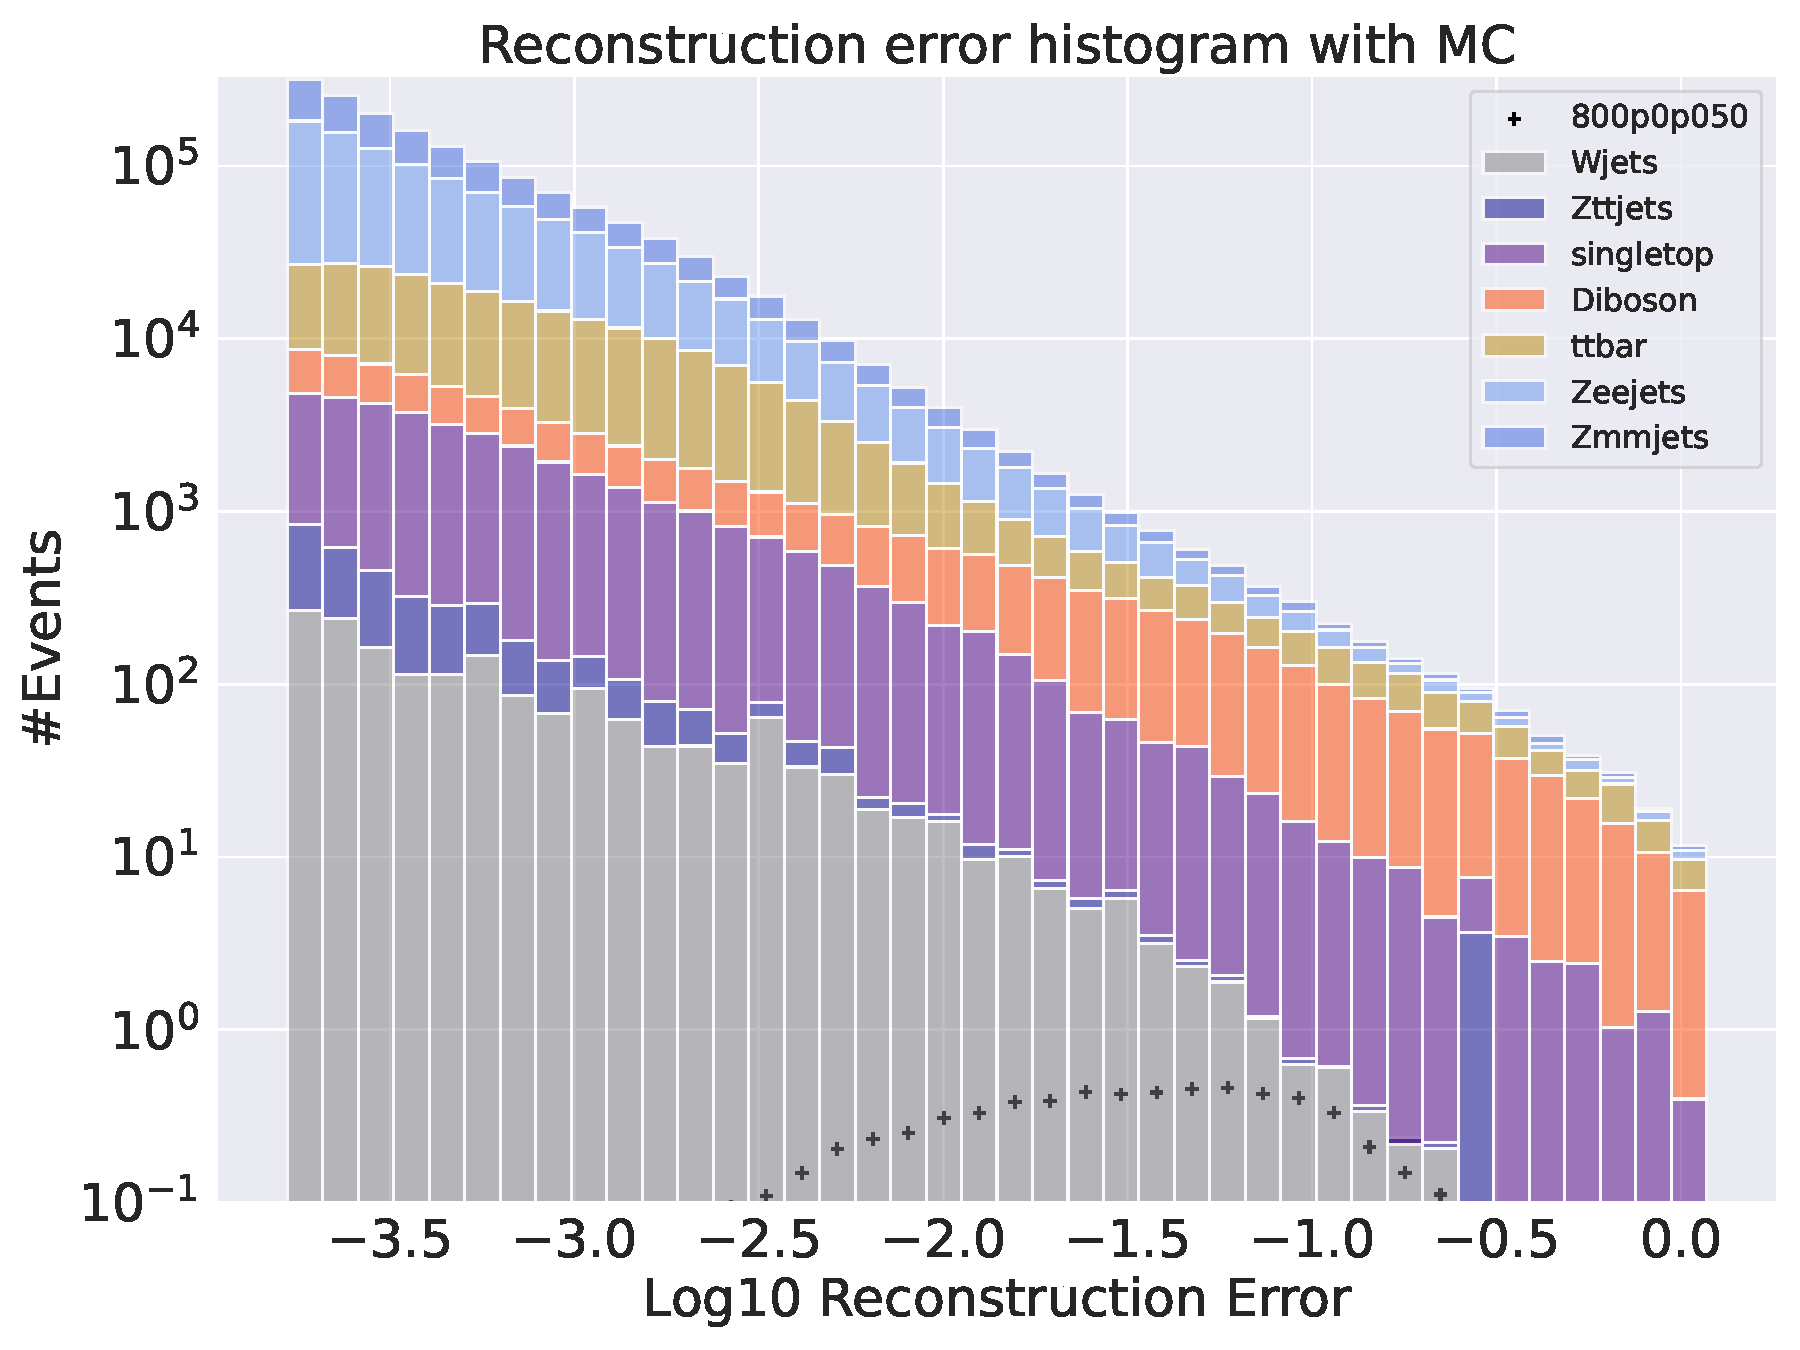
\includegraphics[width=\textwidth]{Figures/AE_testing/big/2lep/b_data_recon_big_rm3_feats_sig_800p0p050_.pdf}
        \caption{ }
        \label{fig:AE_2lep_big_800_2}
    \end{subfigure}
    \hfill
    \begin{subfigure}{.40\textwidth}
        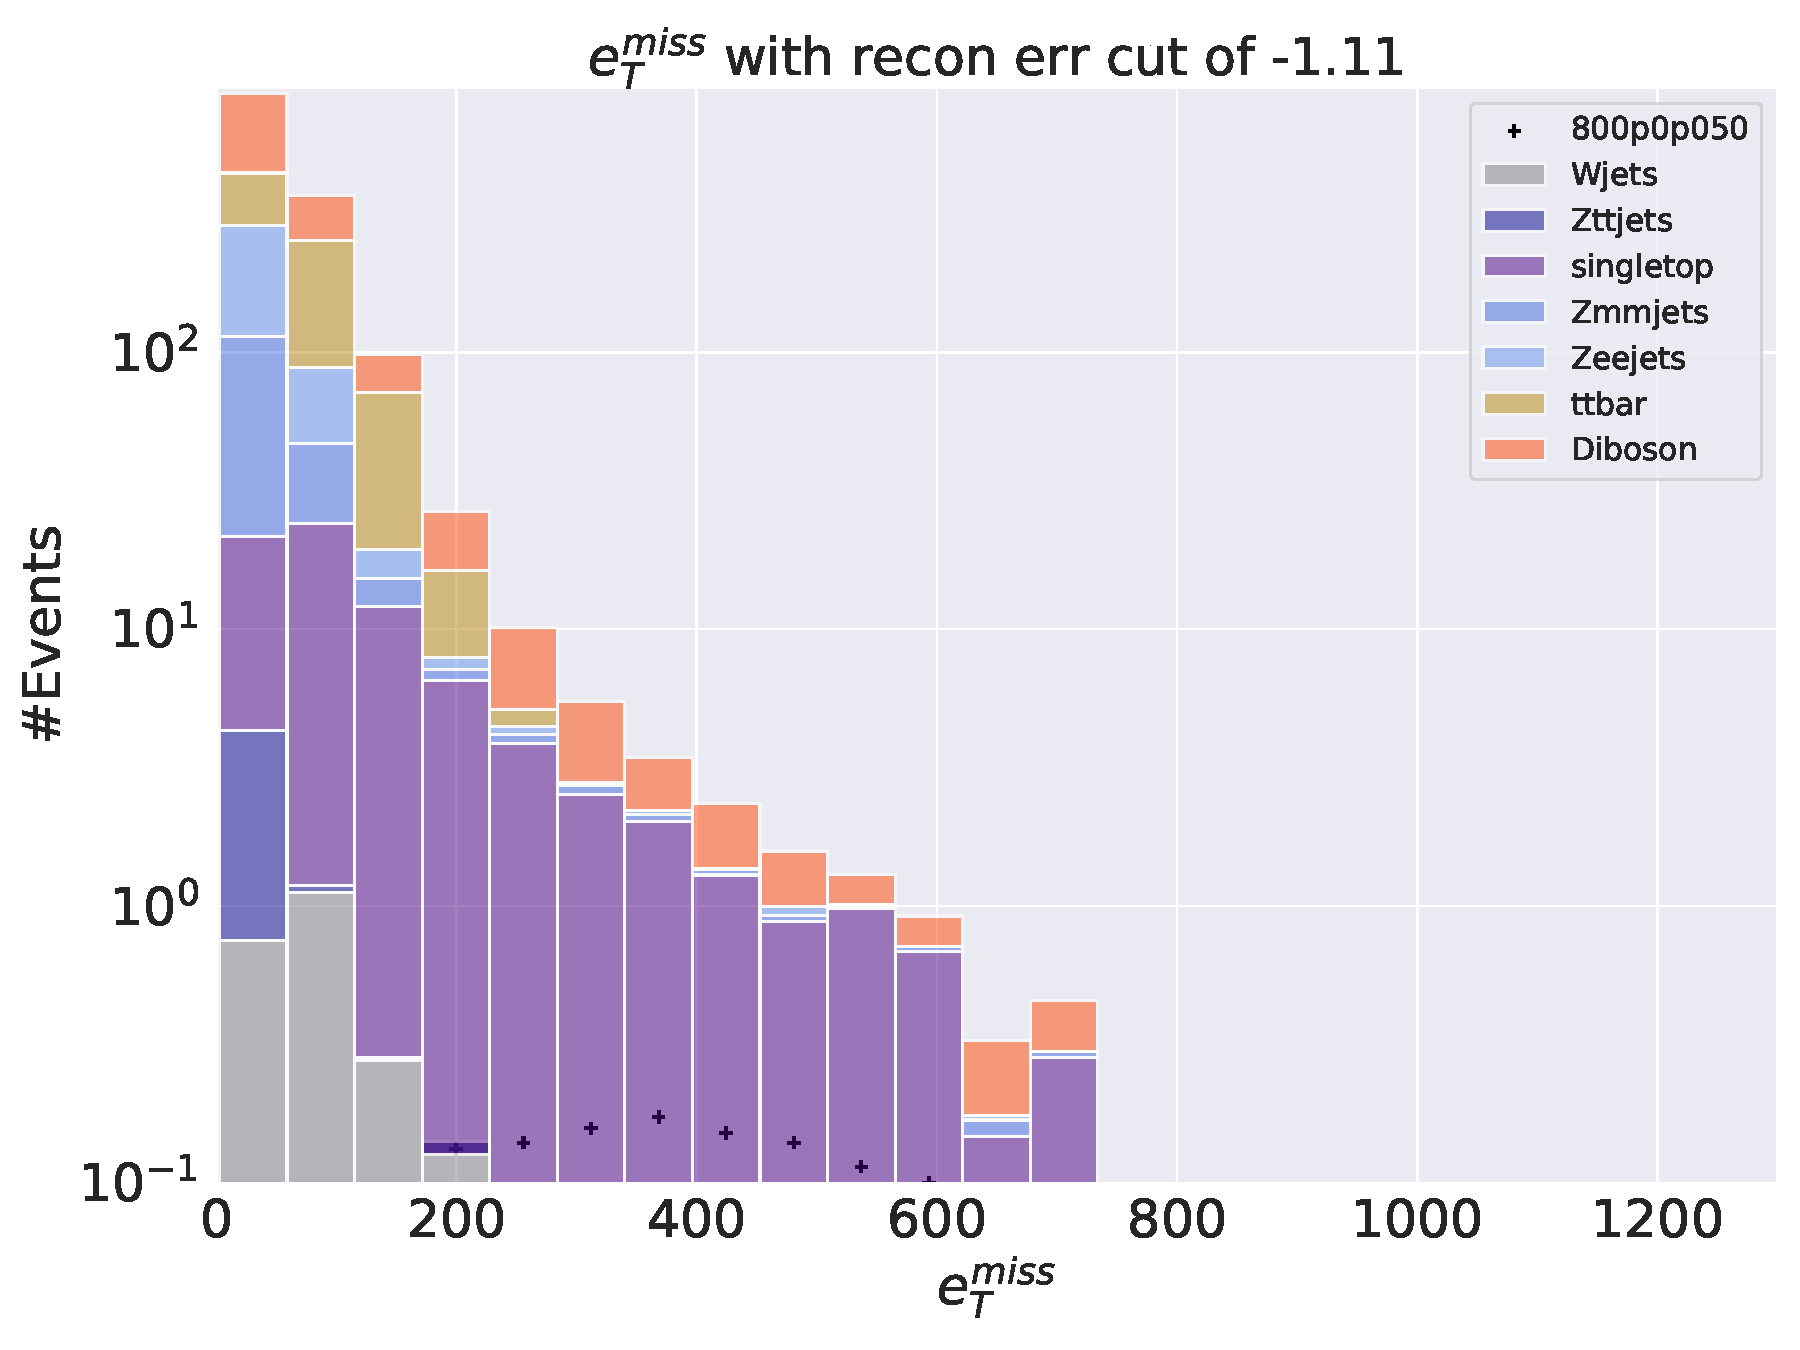
\includegraphics[width=\textwidth]{Figures/AE_testing/big/2lep/b_data_recon_big_rm3_feats_sig_800p0p050_recon_errcut_-1.11.pdf}
        \caption{}
        \label{fig:AE_2lep_big_etmiss_800_2}
    \end{subfigure}
    \hfill
      
    \begin{subfigure}{.40\textwidth}
        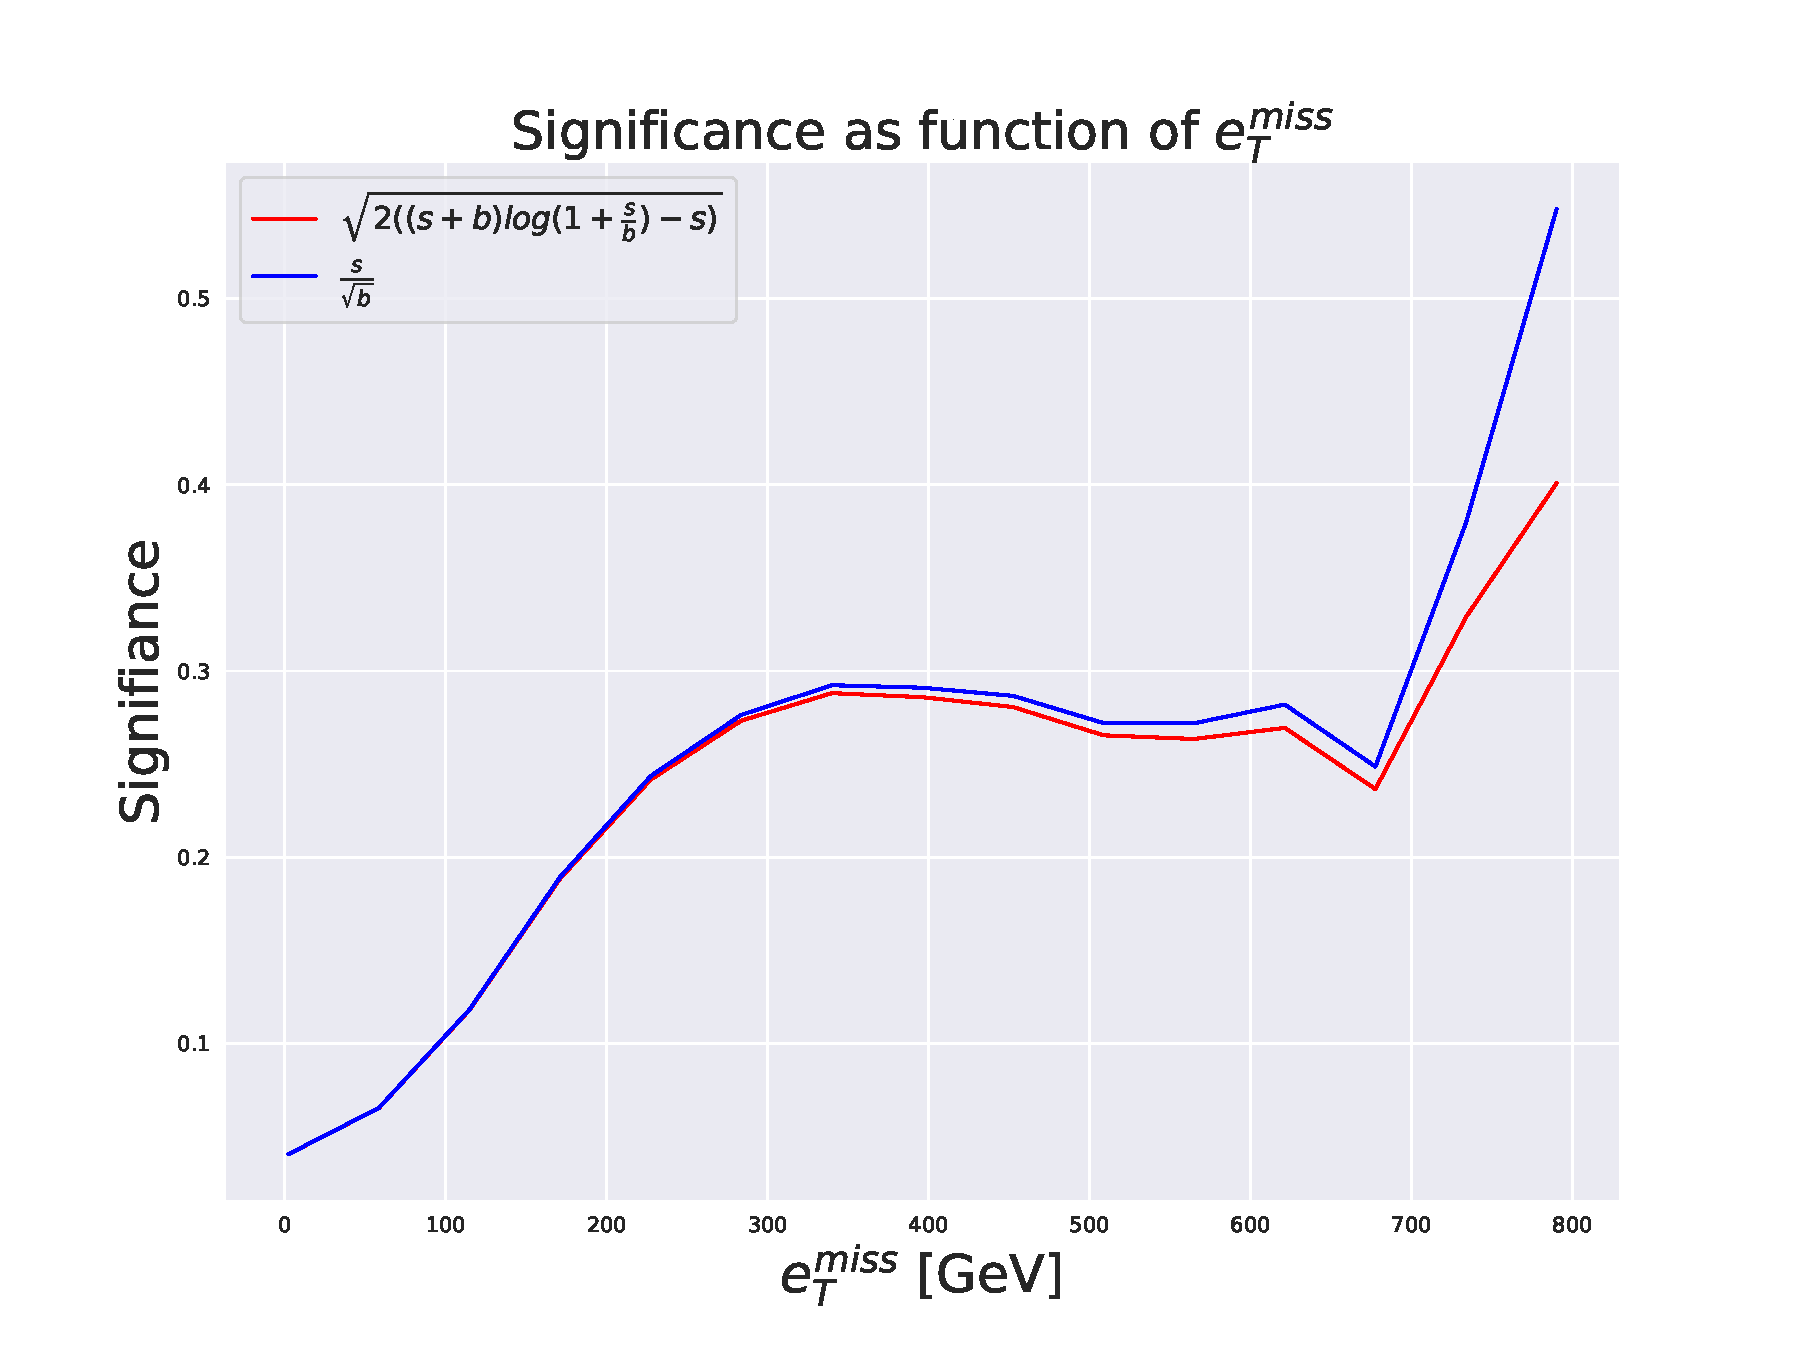
\includegraphics[width=\textwidth]{Figures/AE_testing/big/2lep/significance_etmiss_800p0p050_-1.1125283423037047.pdf}
        \caption{}
        \label{fig:AE_2lep_big_signi_800_2}
    \end{subfigure}
    \hfill      
    \caption[2lep deep network | $800p50$ | AE | 2]{Reconstruction error, $e_T^{miss}$ signal region, $m_{lll}$ signal region and significance as function of 
    $e_T^{miss}$ for the deep regular autoencoder. Here the SUSY $800p50$ model is used.}
    \label{fig:AE_2lep_big_rec_sig_signi_800_2}
\end{figure}

\begin{figure}[H]
    \centering
    \begin{subfigure}{.40\textwidth}
        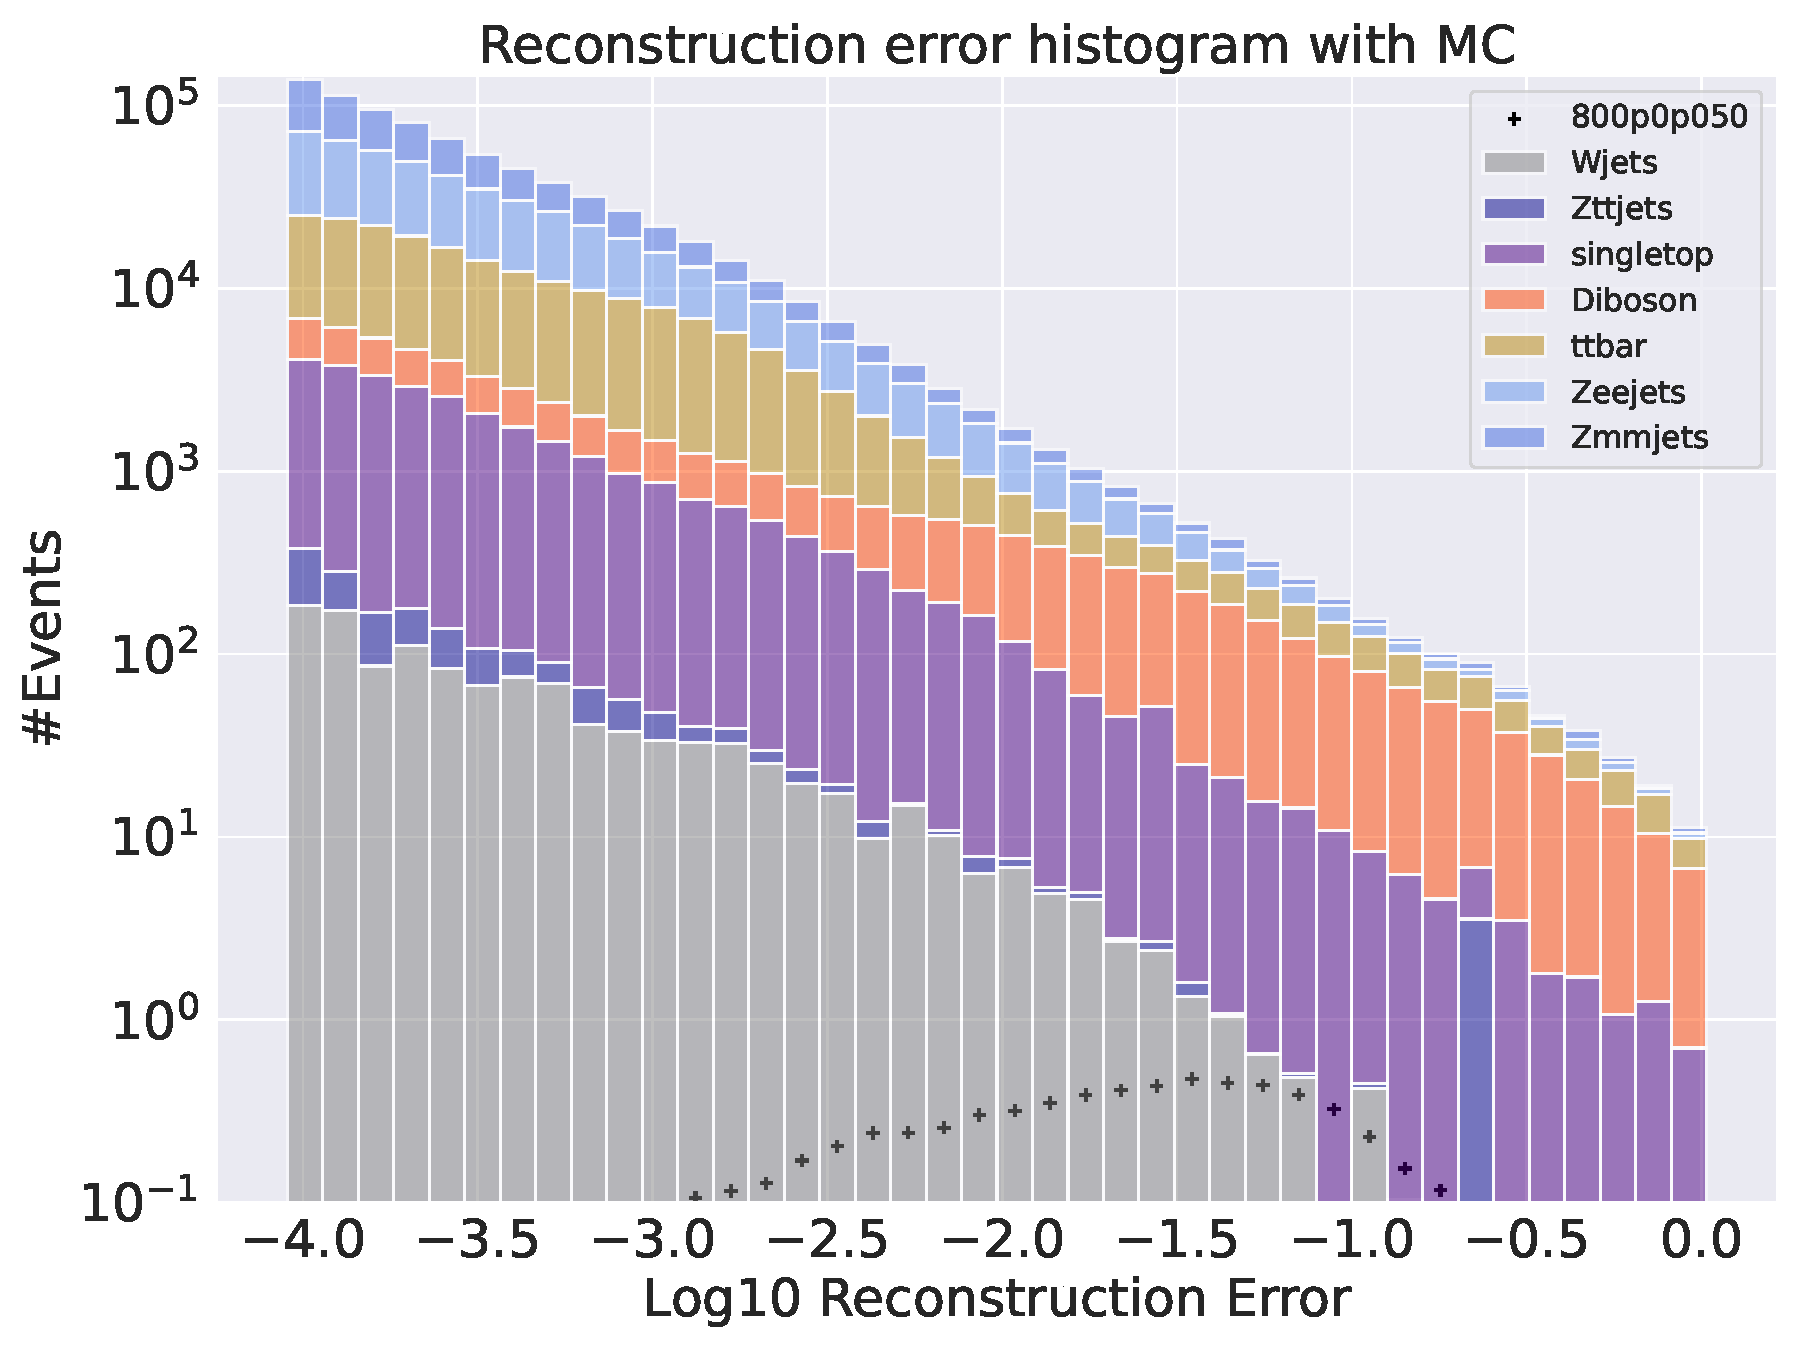
\includegraphics[width=\textwidth]{Figures/AE_testing/small/2lep/b_data_recon_big_rm3_feats_sig_800p0p050_.pdf}
        \caption{ }
        \label{fig:AE_2lep_small_800_2}
    \end{subfigure}
    \hfill
    \begin{subfigure}{.40\textwidth}
        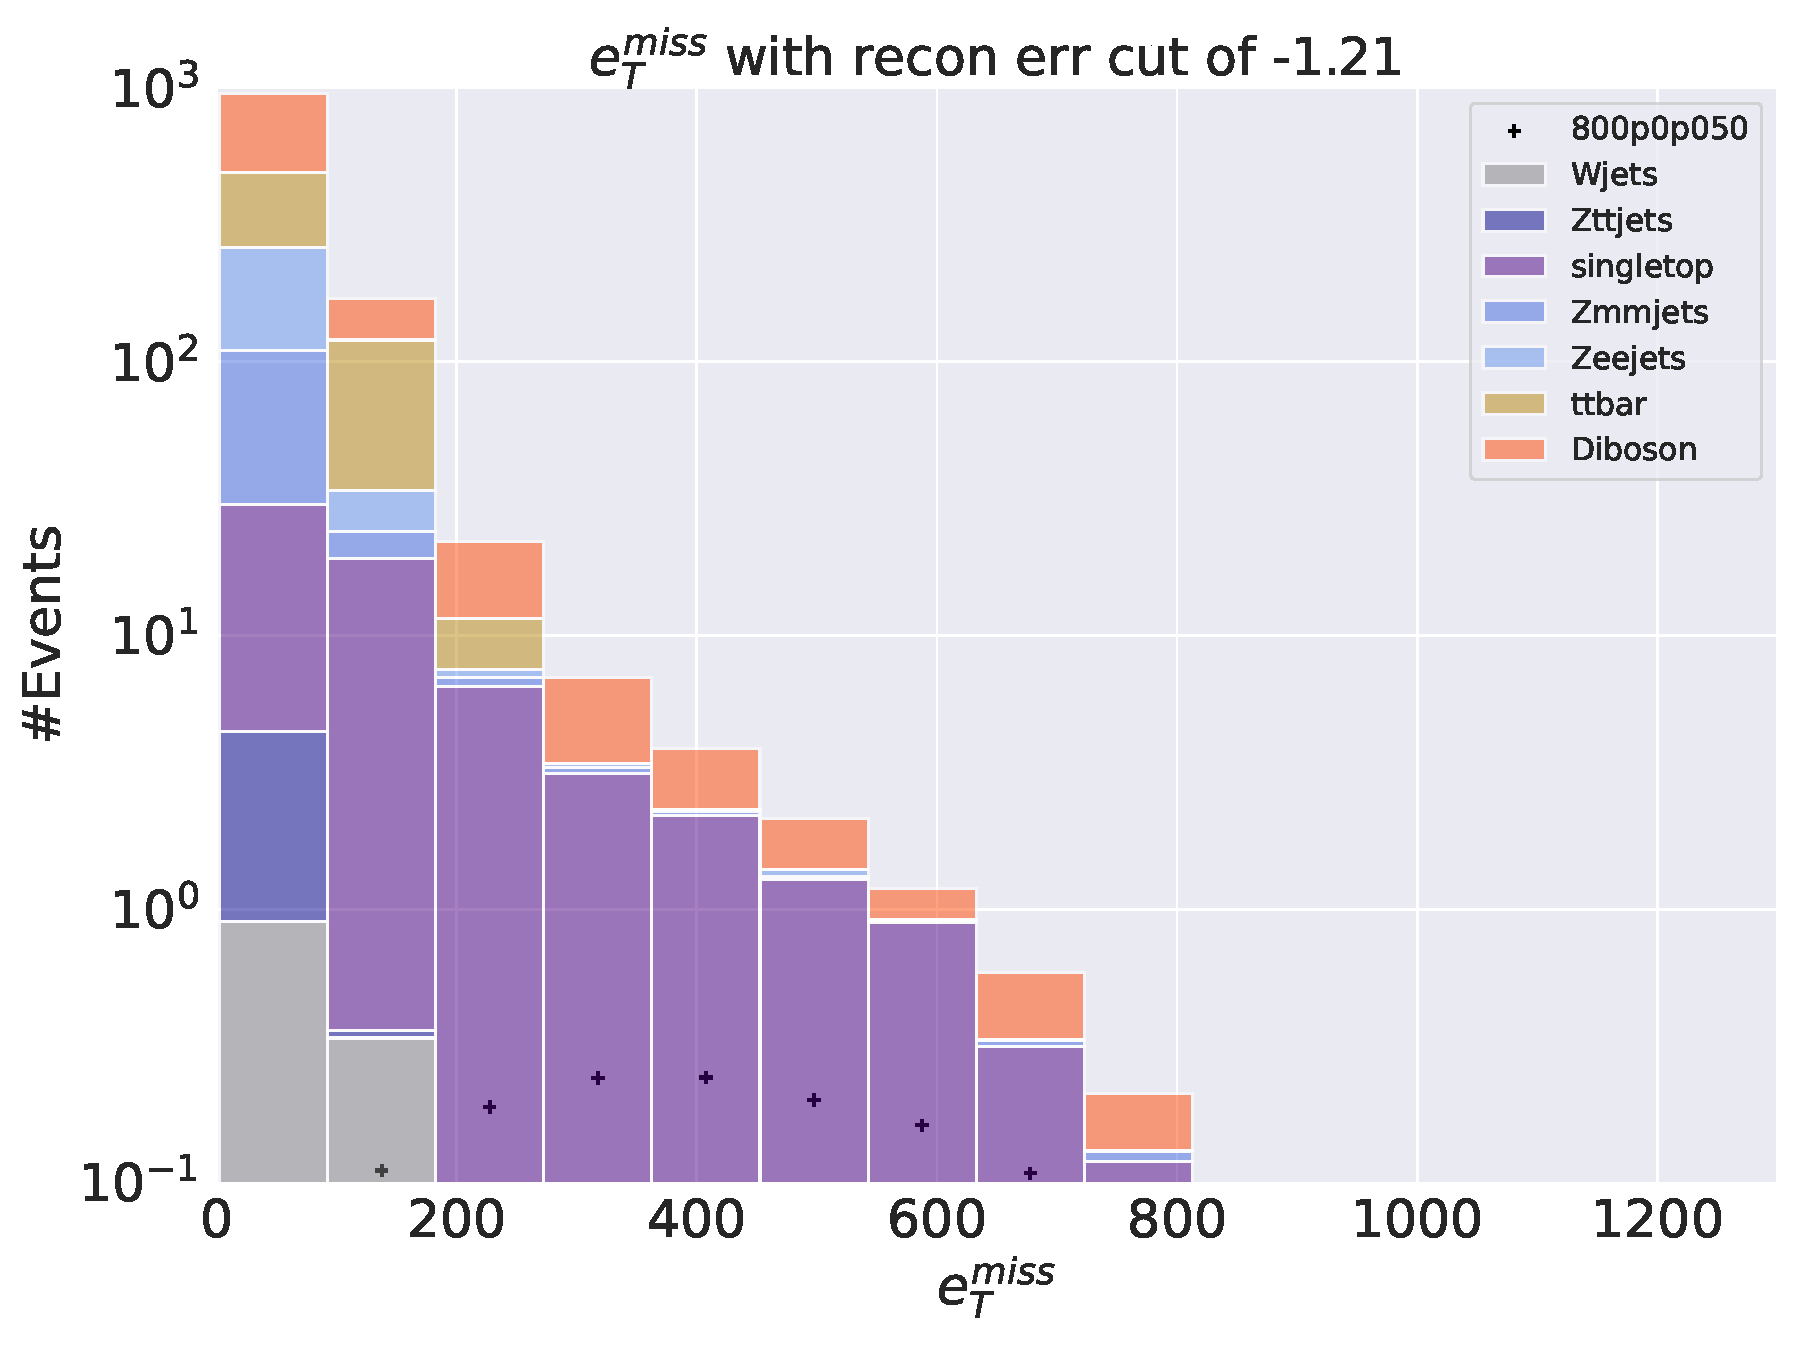
\includegraphics[width=\textwidth]{Figures/AE_testing/small/2lep/b_data_recon_big_rm3_feats_sig_800p0p050_recon_errcut_-1.21.pdf}
        \caption{}
        \label{fig:AE_2lep_small_etmiss_800_2}
    \end{subfigure}
    \hfill  
    \begin{subfigure}{.40\textwidth}
        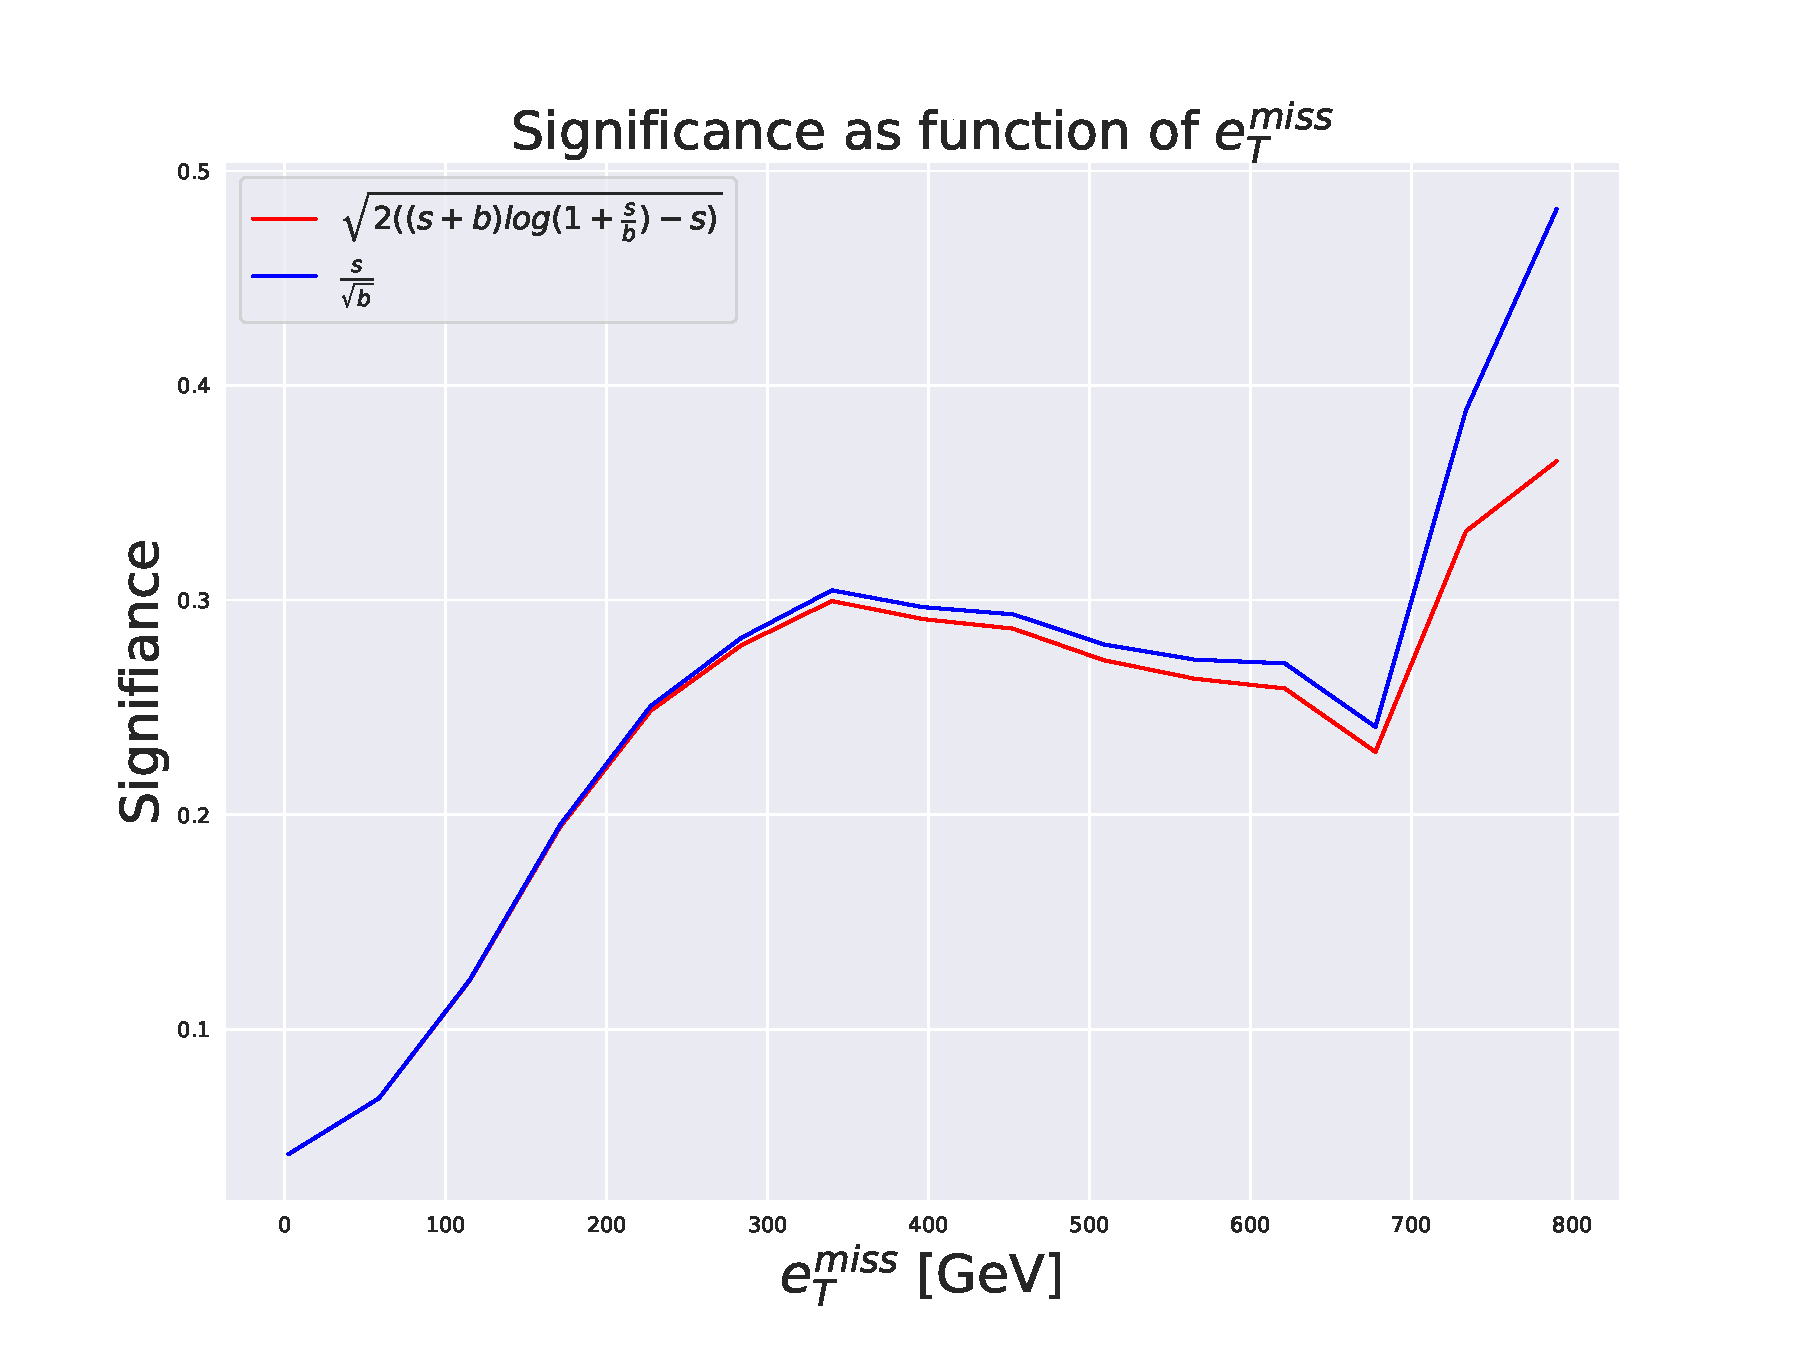
\includegraphics[width=\textwidth]{Figures/AE_testing/small/2lep/significance_etmiss_800p0p050_-1.2087791708604207.pdf}
        \caption{}
        \label{fig:AE_2lep_small_signi_800_2}
    \end{subfigure}
    \hfill      
    \caption[2lep shallow network | $800p50$ | AE | 2]{Reconstruction error, $e_T^{miss}$ signal region, $m_{lll}$ signal region and significance as function of 
    $e_T^{miss}$ for the shallow regular autoencoder. Here the SUSY $800p50$ model is used.}
    \label{fig:AE_2lep_small_rec_sig_signi_800_2}
\end{figure}
























\begin{figure}[H]
    \centering
    \begin{subfigure}{.40\textwidth}
        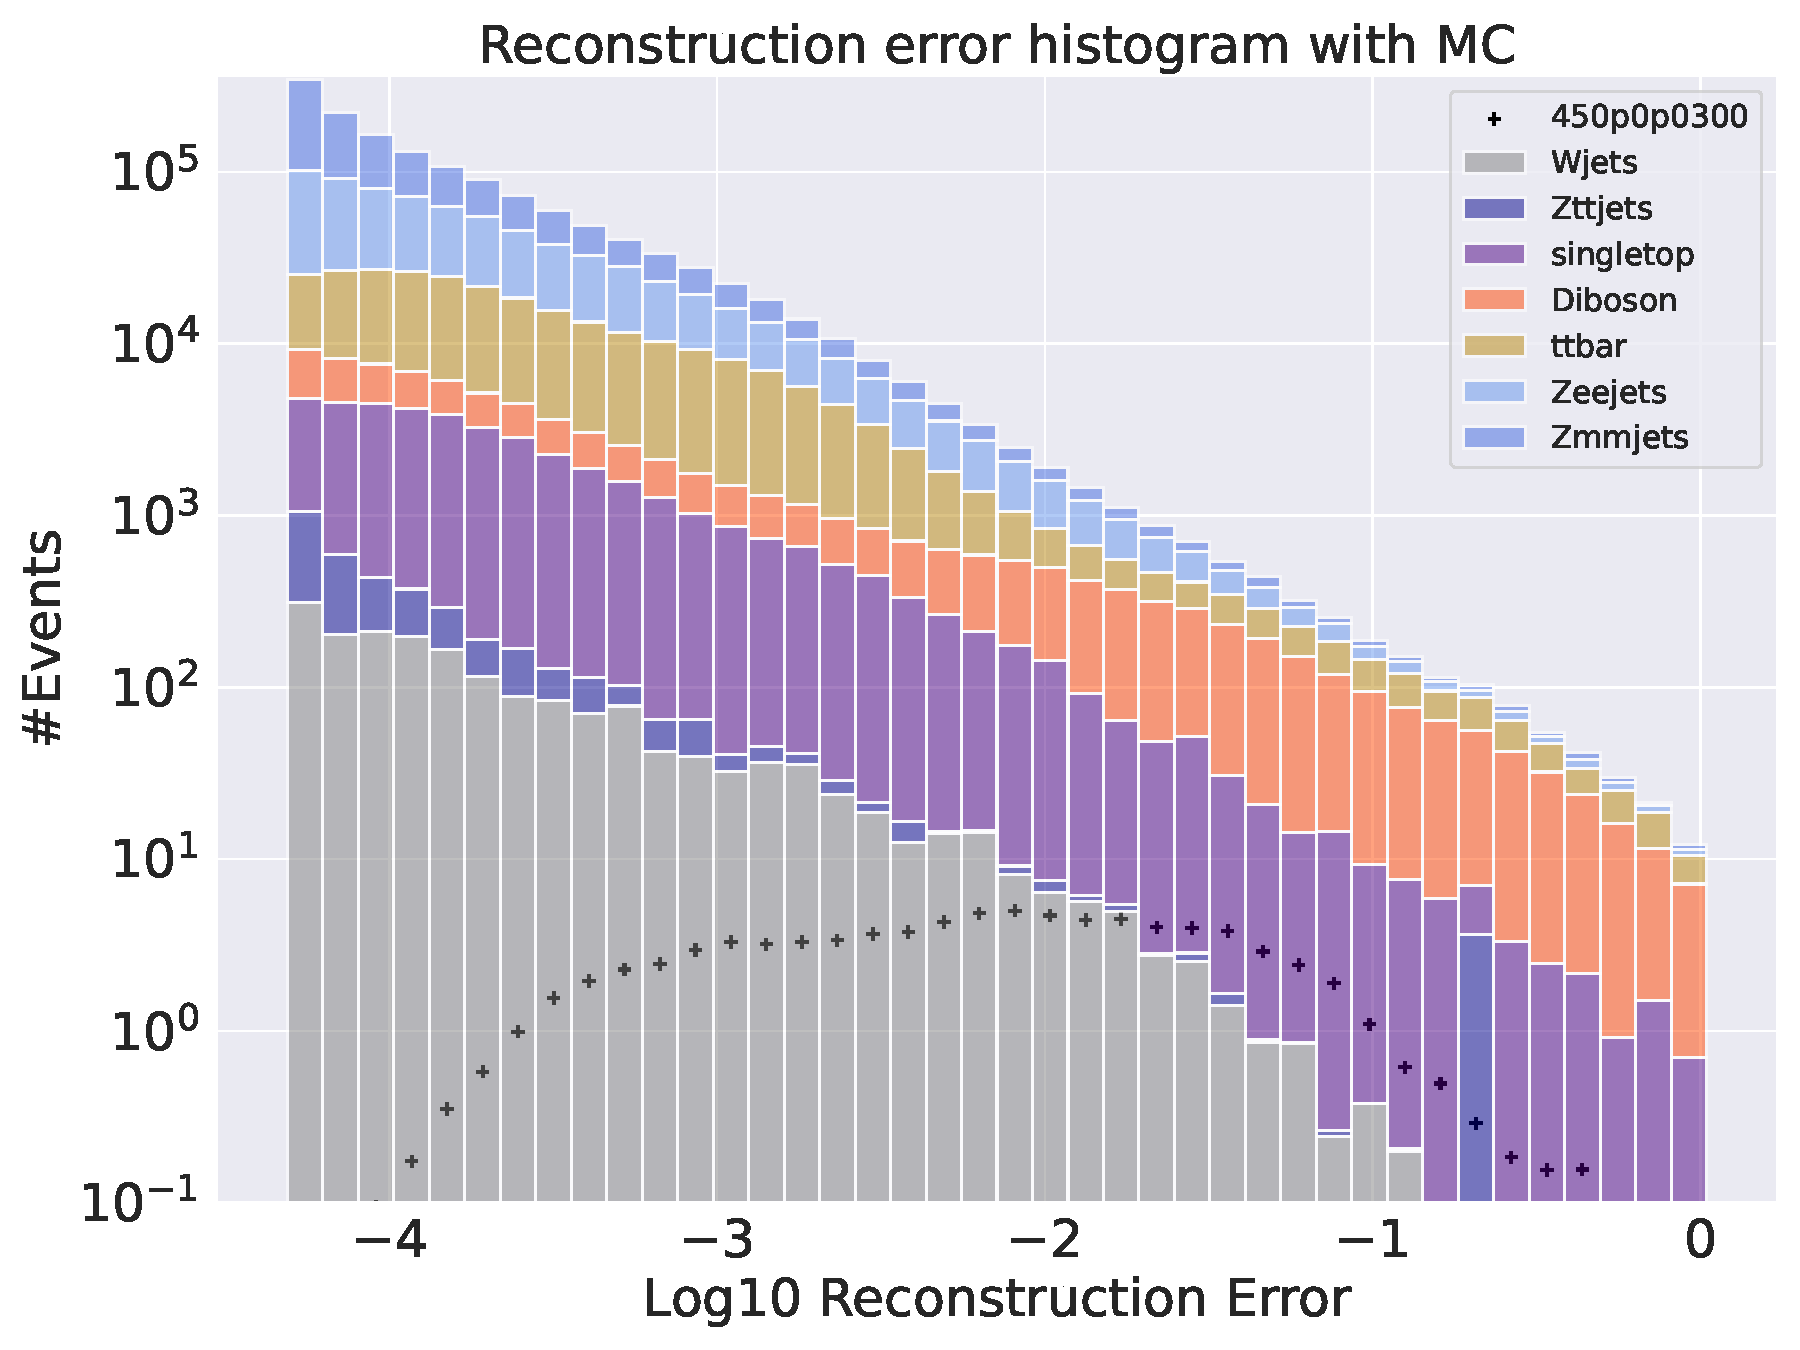
\includegraphics[width=\textwidth]{Figures/AE_testing/small/2lep/b_data_recon_big_rm3_feats_sig_450p0p0300_.pdf}
        \caption{ }
        \label{fig:AE_2lep_big_450_3}
    \end{subfigure}
    \hfill
    \begin{subfigure}{.40\textwidth}
        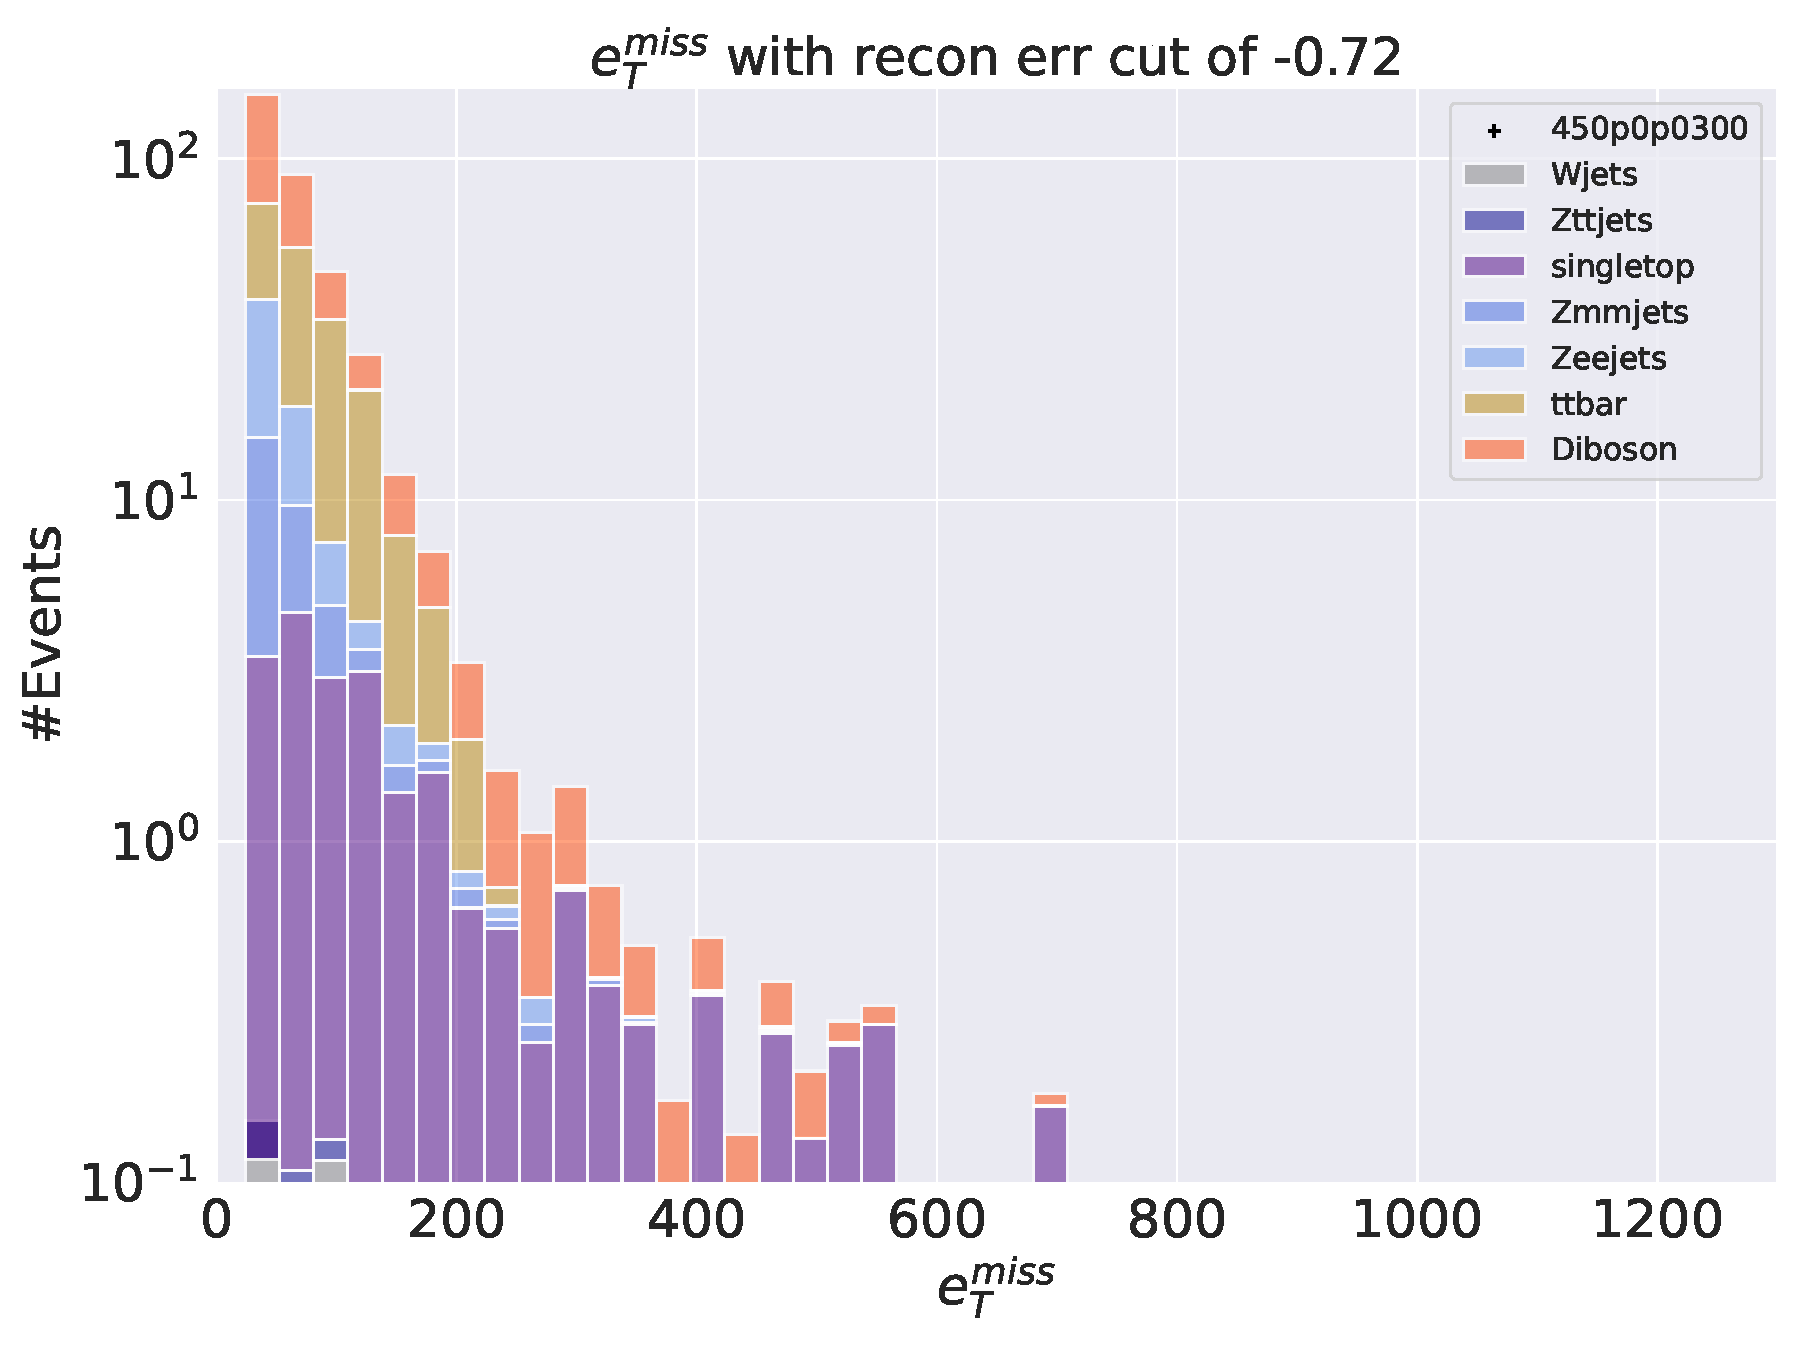
\includegraphics[width=\textwidth]{Figures/AE_testing/big/2lep/b_data_recon_big_rm3_feats_sig_450p0p0300_recon_errcut_-0.72.pdf}
        \caption{}
        \label{fig:AE_2lep_big_etmiss_450_3}
    \end{subfigure}
    \hfill 
    \begin{subfigure}{.40\textwidth}
        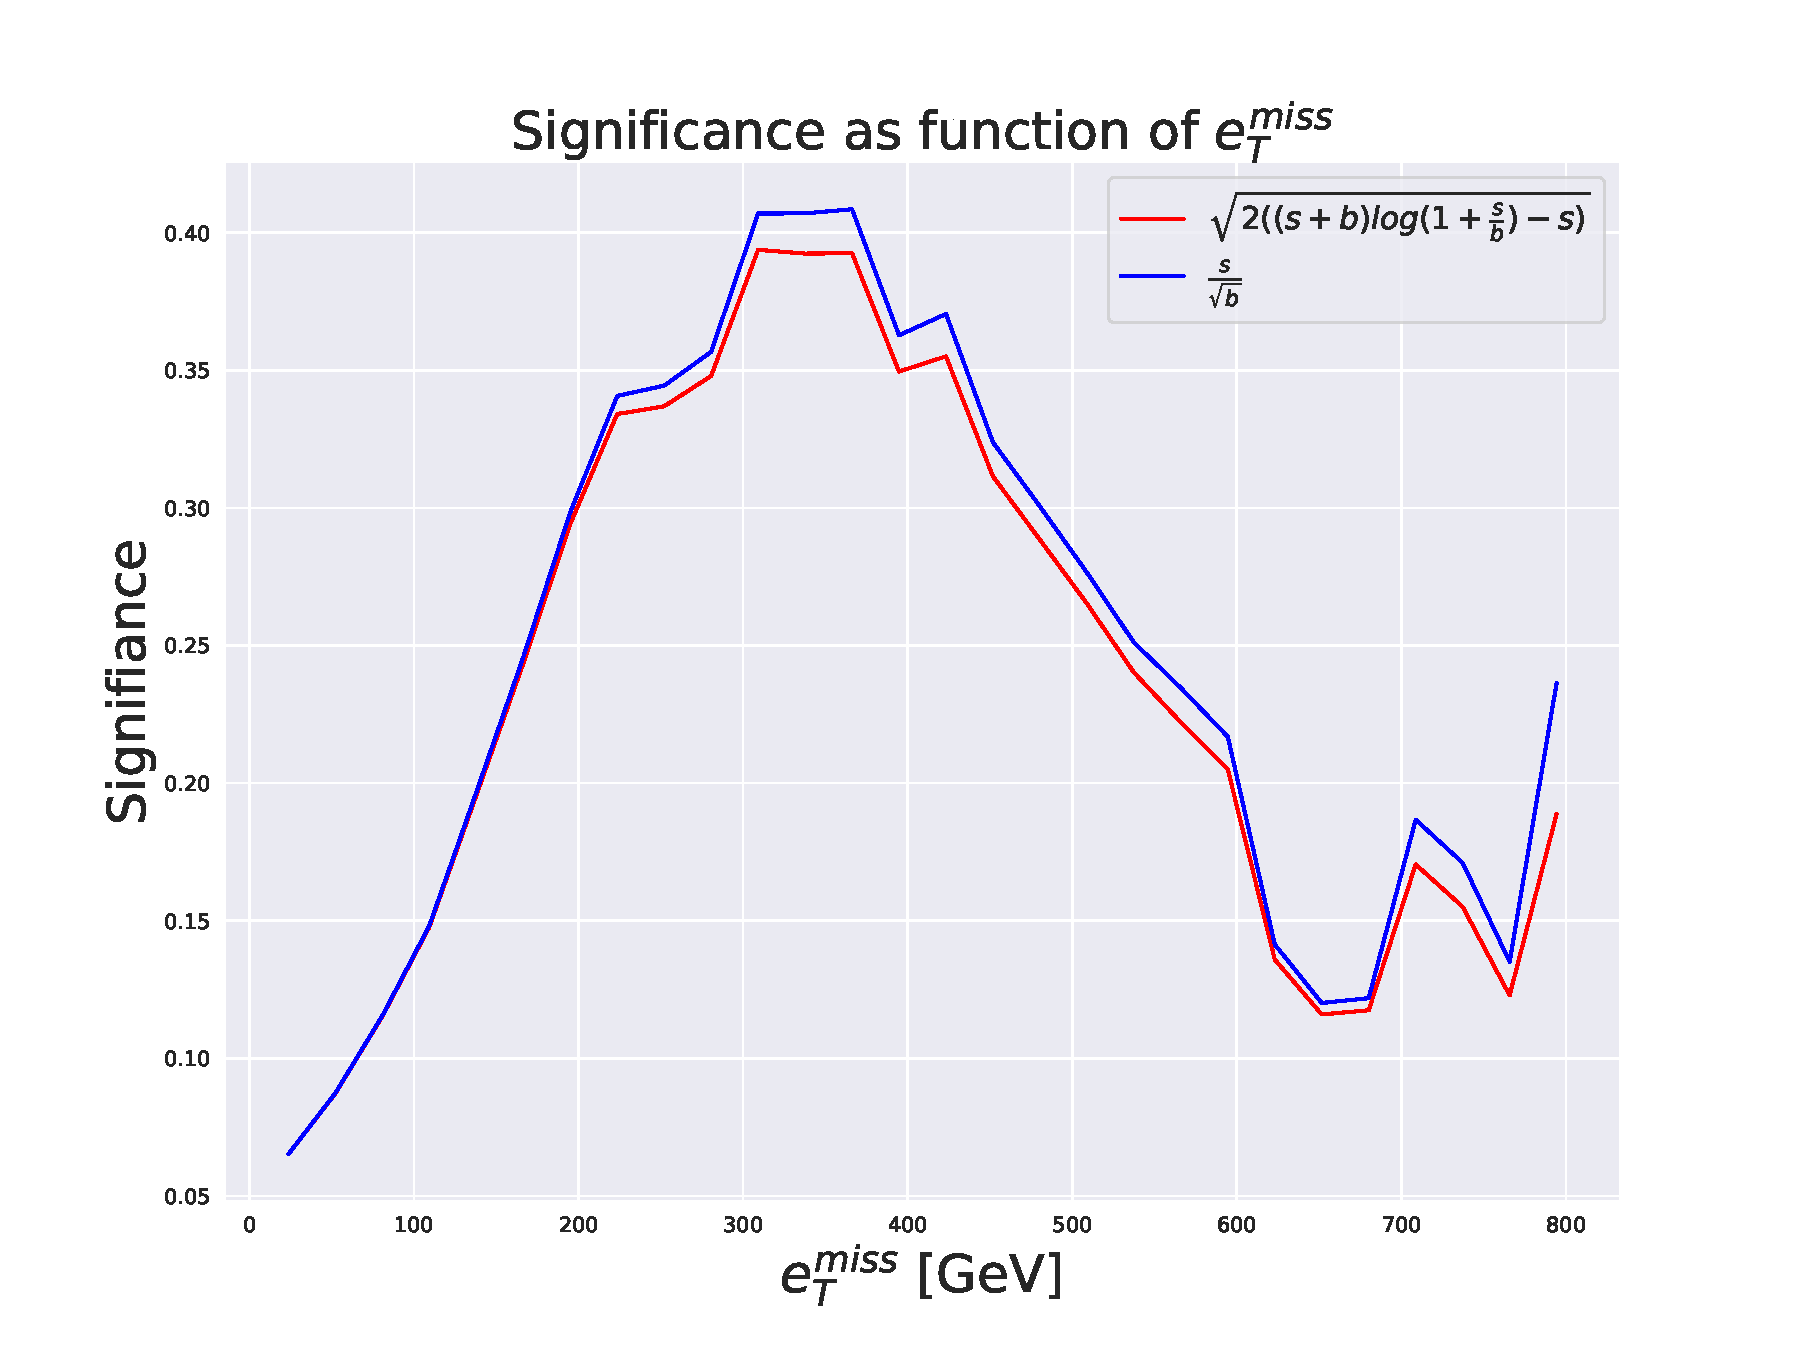
\includegraphics[width=\textwidth]{Figures/AE_testing/big/2lep/significance_etmiss_450p0p0300_-0.7180276969063684.pdf}
        \caption{}
        \label{fig:AE_2lep_big_signi_450_3}
    \end{subfigure}
    \hfill      
    \caption[2lep deep network | $450p300$ | AE | 3]{Reconstruction error, $e_T^{miss}$ signal region, $m_{lll}$ signal region and significance as function of 
    $e_T^{miss}$ for the deep regular autoencoder. Here the SUSY $450p300$ model is used.}
    \label{fig:AE_2lep_big_rec_sig_signi_450_3}
\end{figure}

\begin{figure}[H]
    \centering
    \begin{subfigure}{.40\textwidth}
        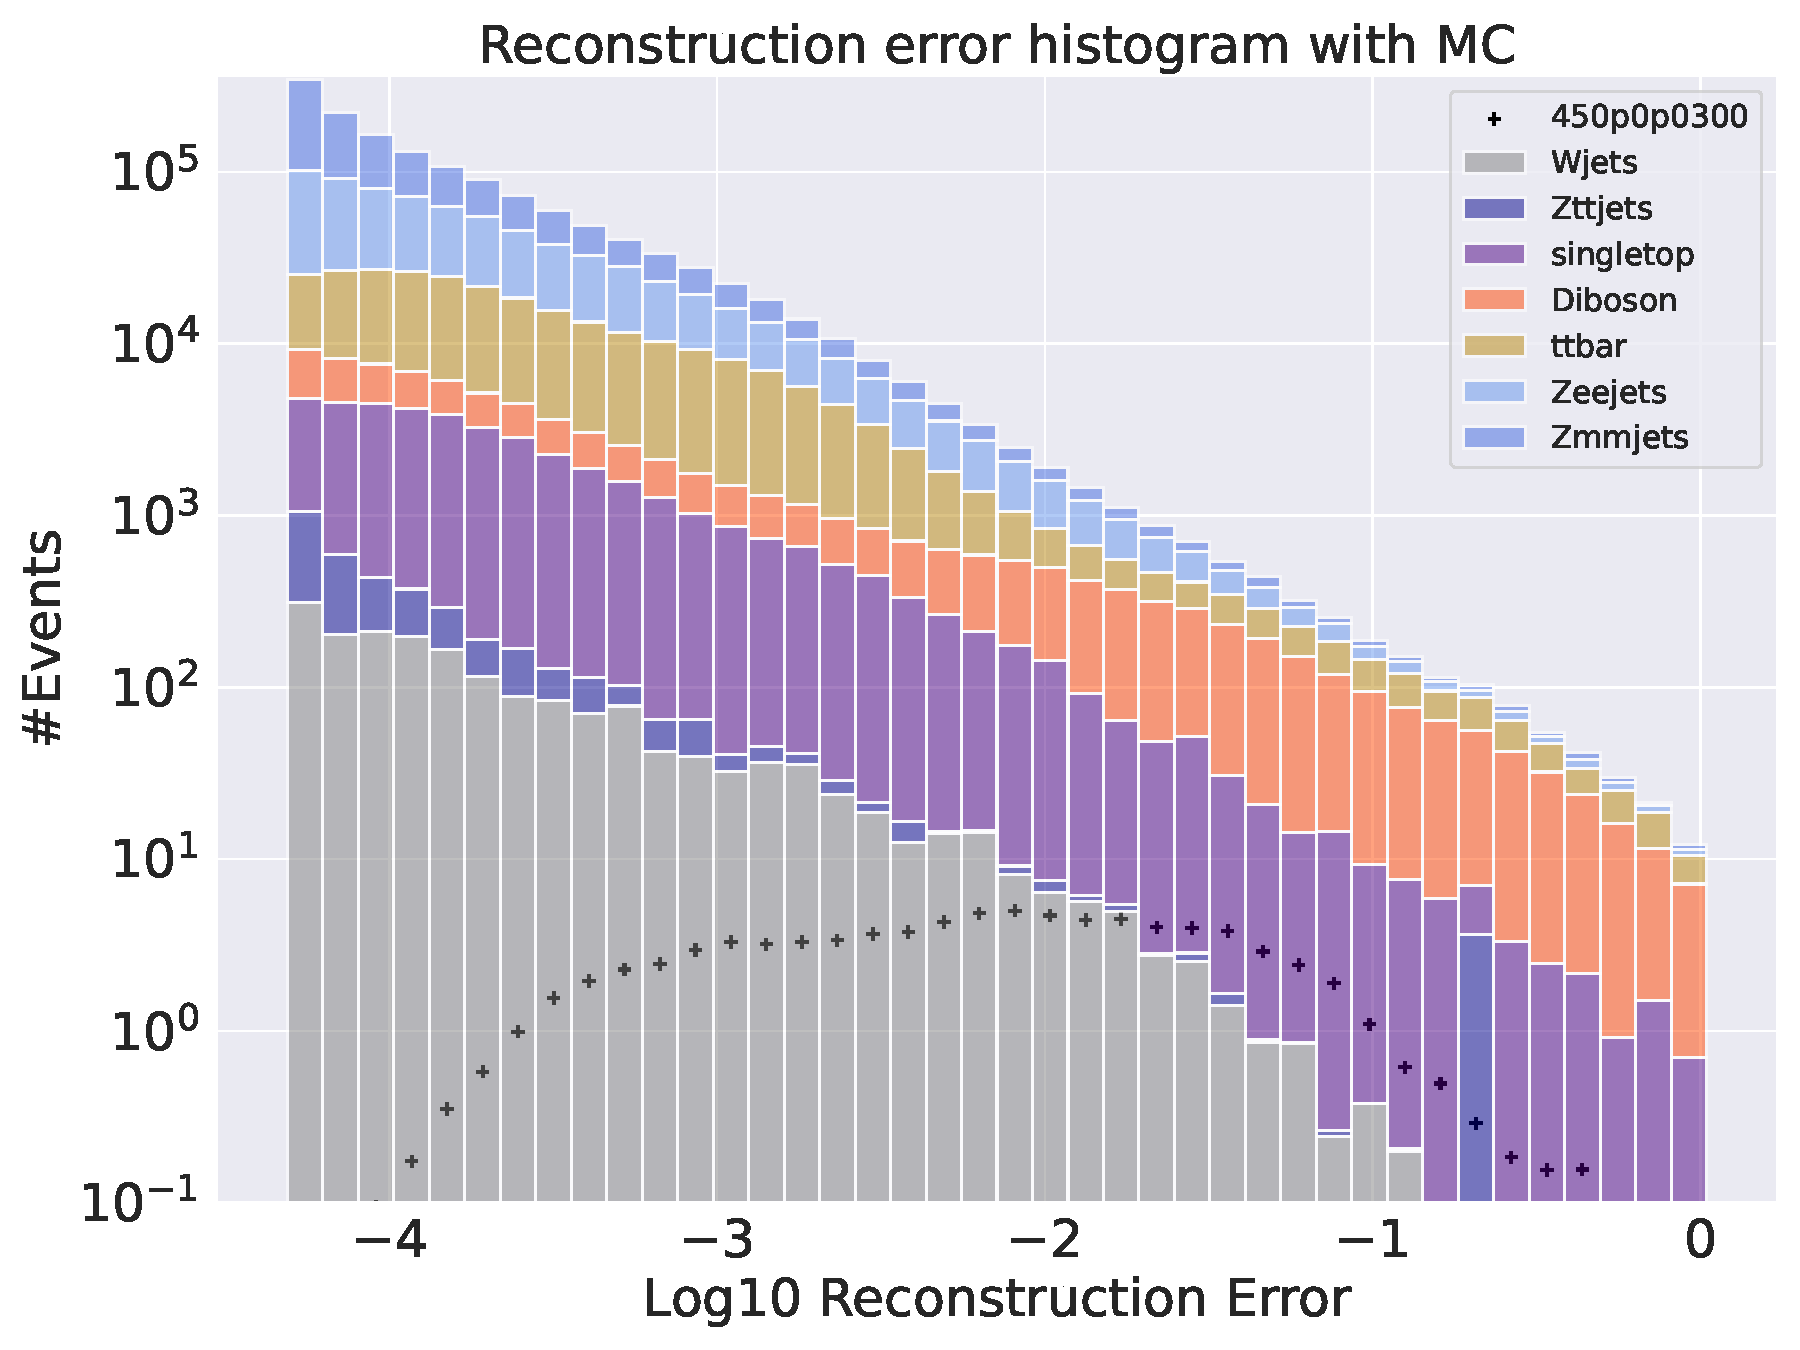
\includegraphics[width=\textwidth]{Figures/AE_testing/small/2lep/b_data_recon_big_rm3_feats_sig_450p0p0300_.pdf}
        \caption{ }
        \label{fig:AE_2lep_small_450_3}
    \end{subfigure}
    \hfill
    \begin{subfigure}{.40\textwidth}
        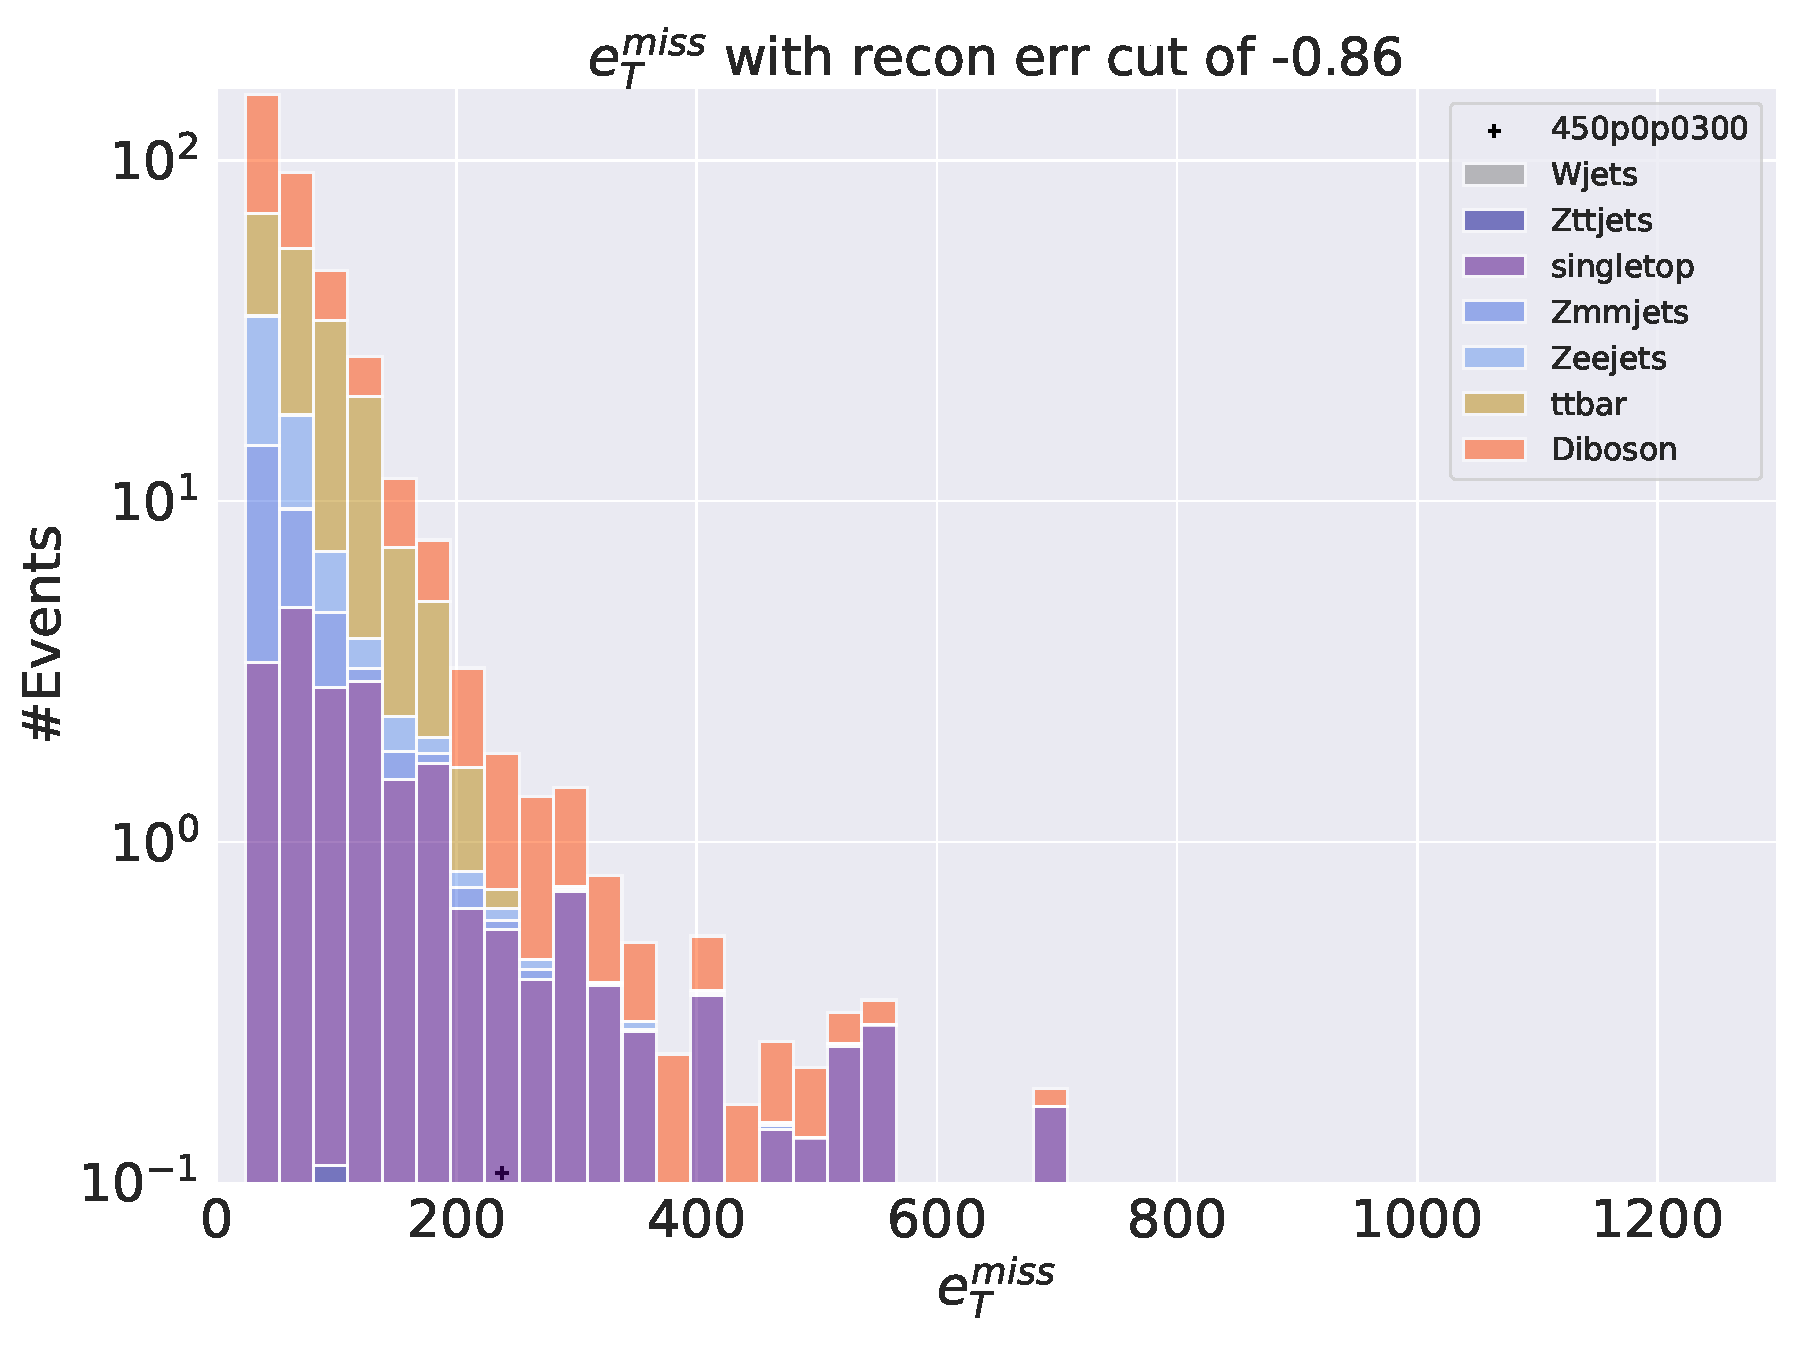
\includegraphics[width=\textwidth]{Figures/AE_testing/small/2lep/b_data_recon_big_rm3_feats_sig_450p0p0300_recon_errcut_-0.86.pdf}
        \caption{}
        \label{fig:AE_2lep_small_etmiss_450_3}
    \end{subfigure}
    \hfill  
    \begin{subfigure}{.40\textwidth}
        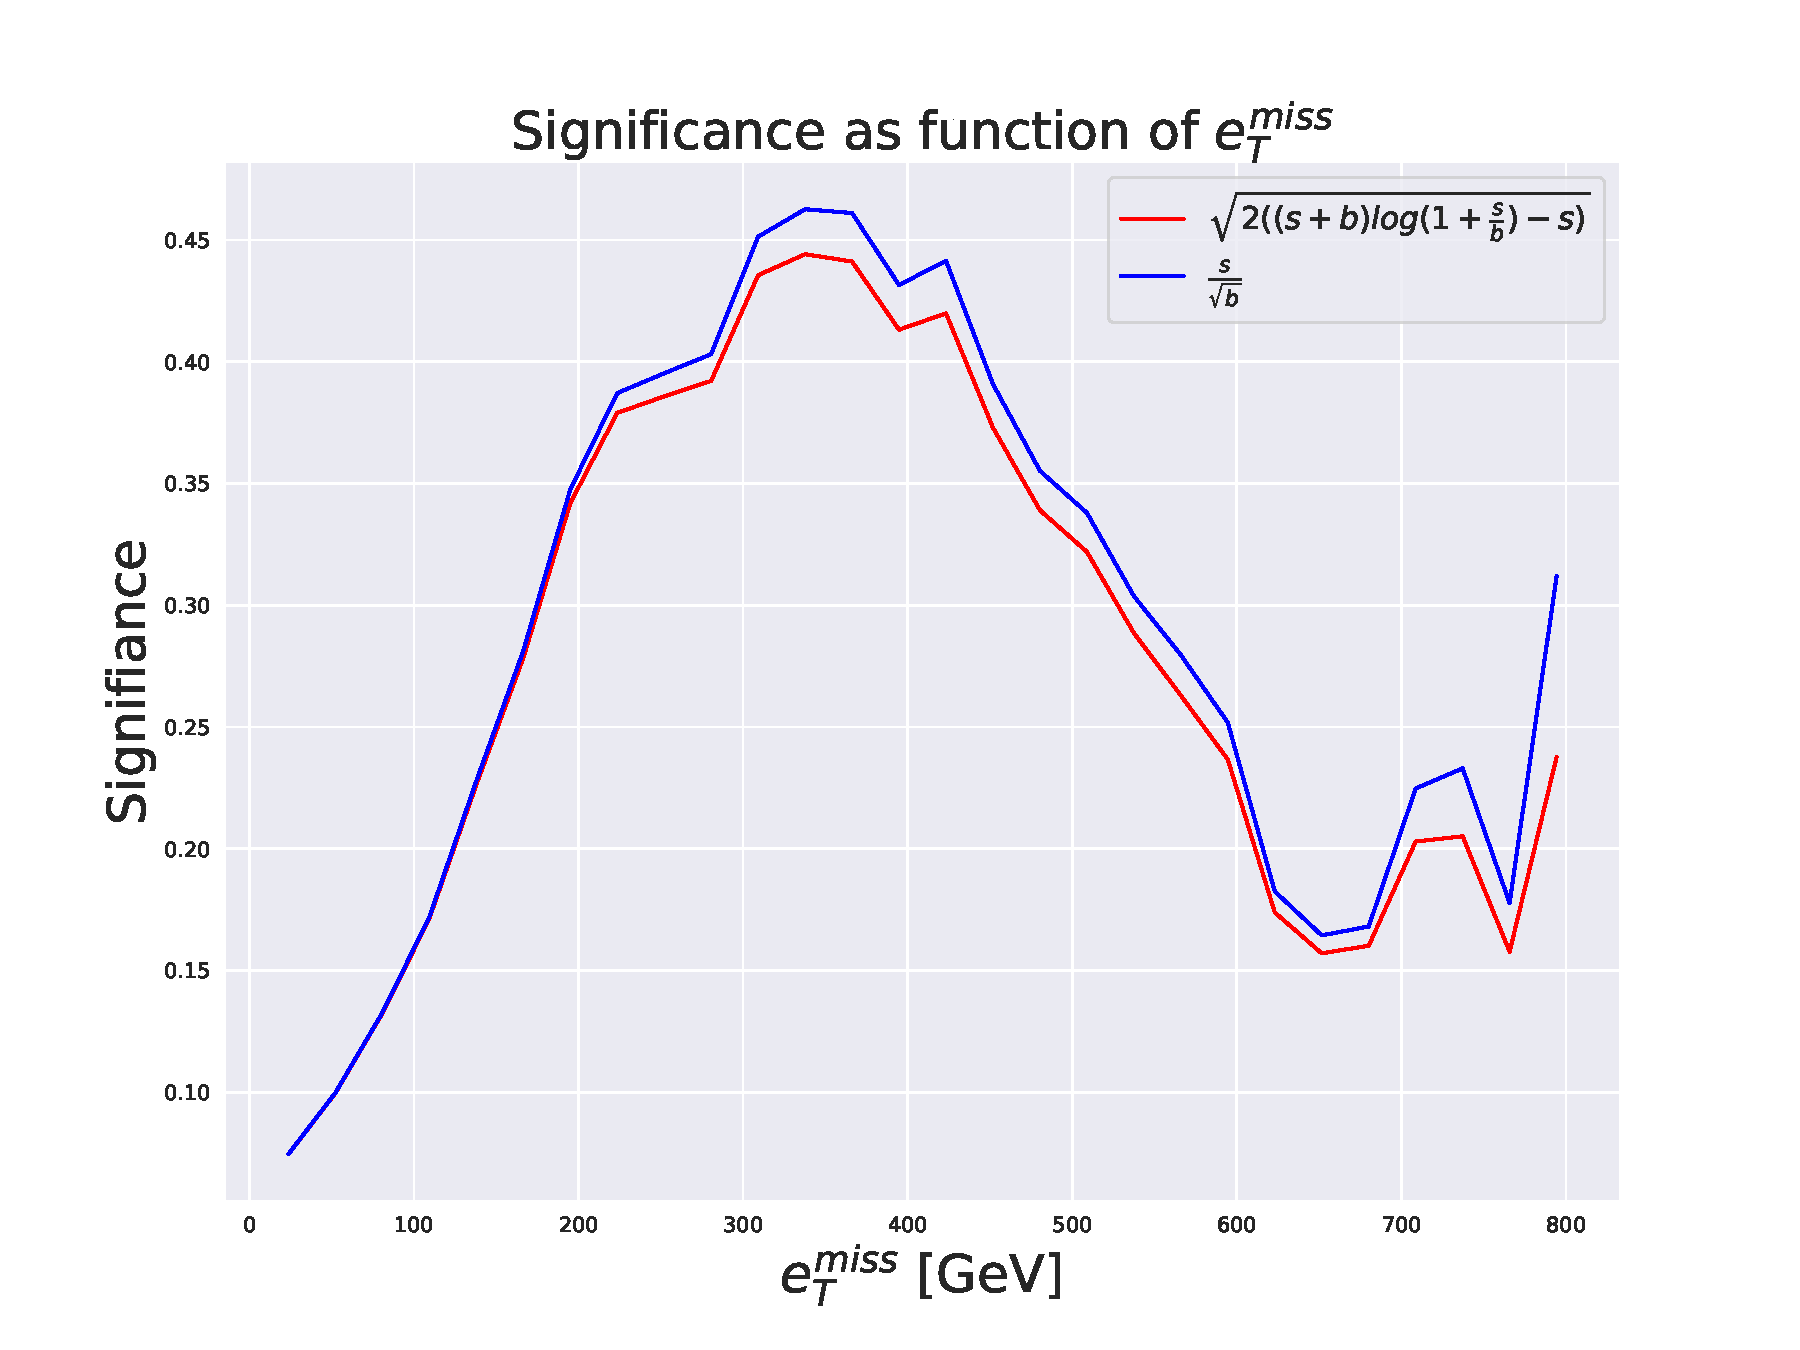
\includegraphics[width=\textwidth]{Figures/AE_testing/small/2lep/significance_etmiss_450p0p0300_-0.8583753266807368.pdf}
        \caption{}
        \label{fig:AE_2lep_small_signi_450_3}
    \end{subfigure}
    \hfill      
    \caption[2lep shallow network | $450p300$ | AE | 3]{Reconstruction error, $e_T^{miss}$ signal region, $m_{lll}$ signal region and significance as function of 
    $e_T^{miss}$ for the deep regular autoencoder. Here the SUSY $450p300$ model is used.}
    \label{fig:AE_2lep_small_rec_sig_signi_450_3}
\end{figure}


\begin{figure}[H]
    \centering
    \begin{subfigure}{.40\textwidth}
        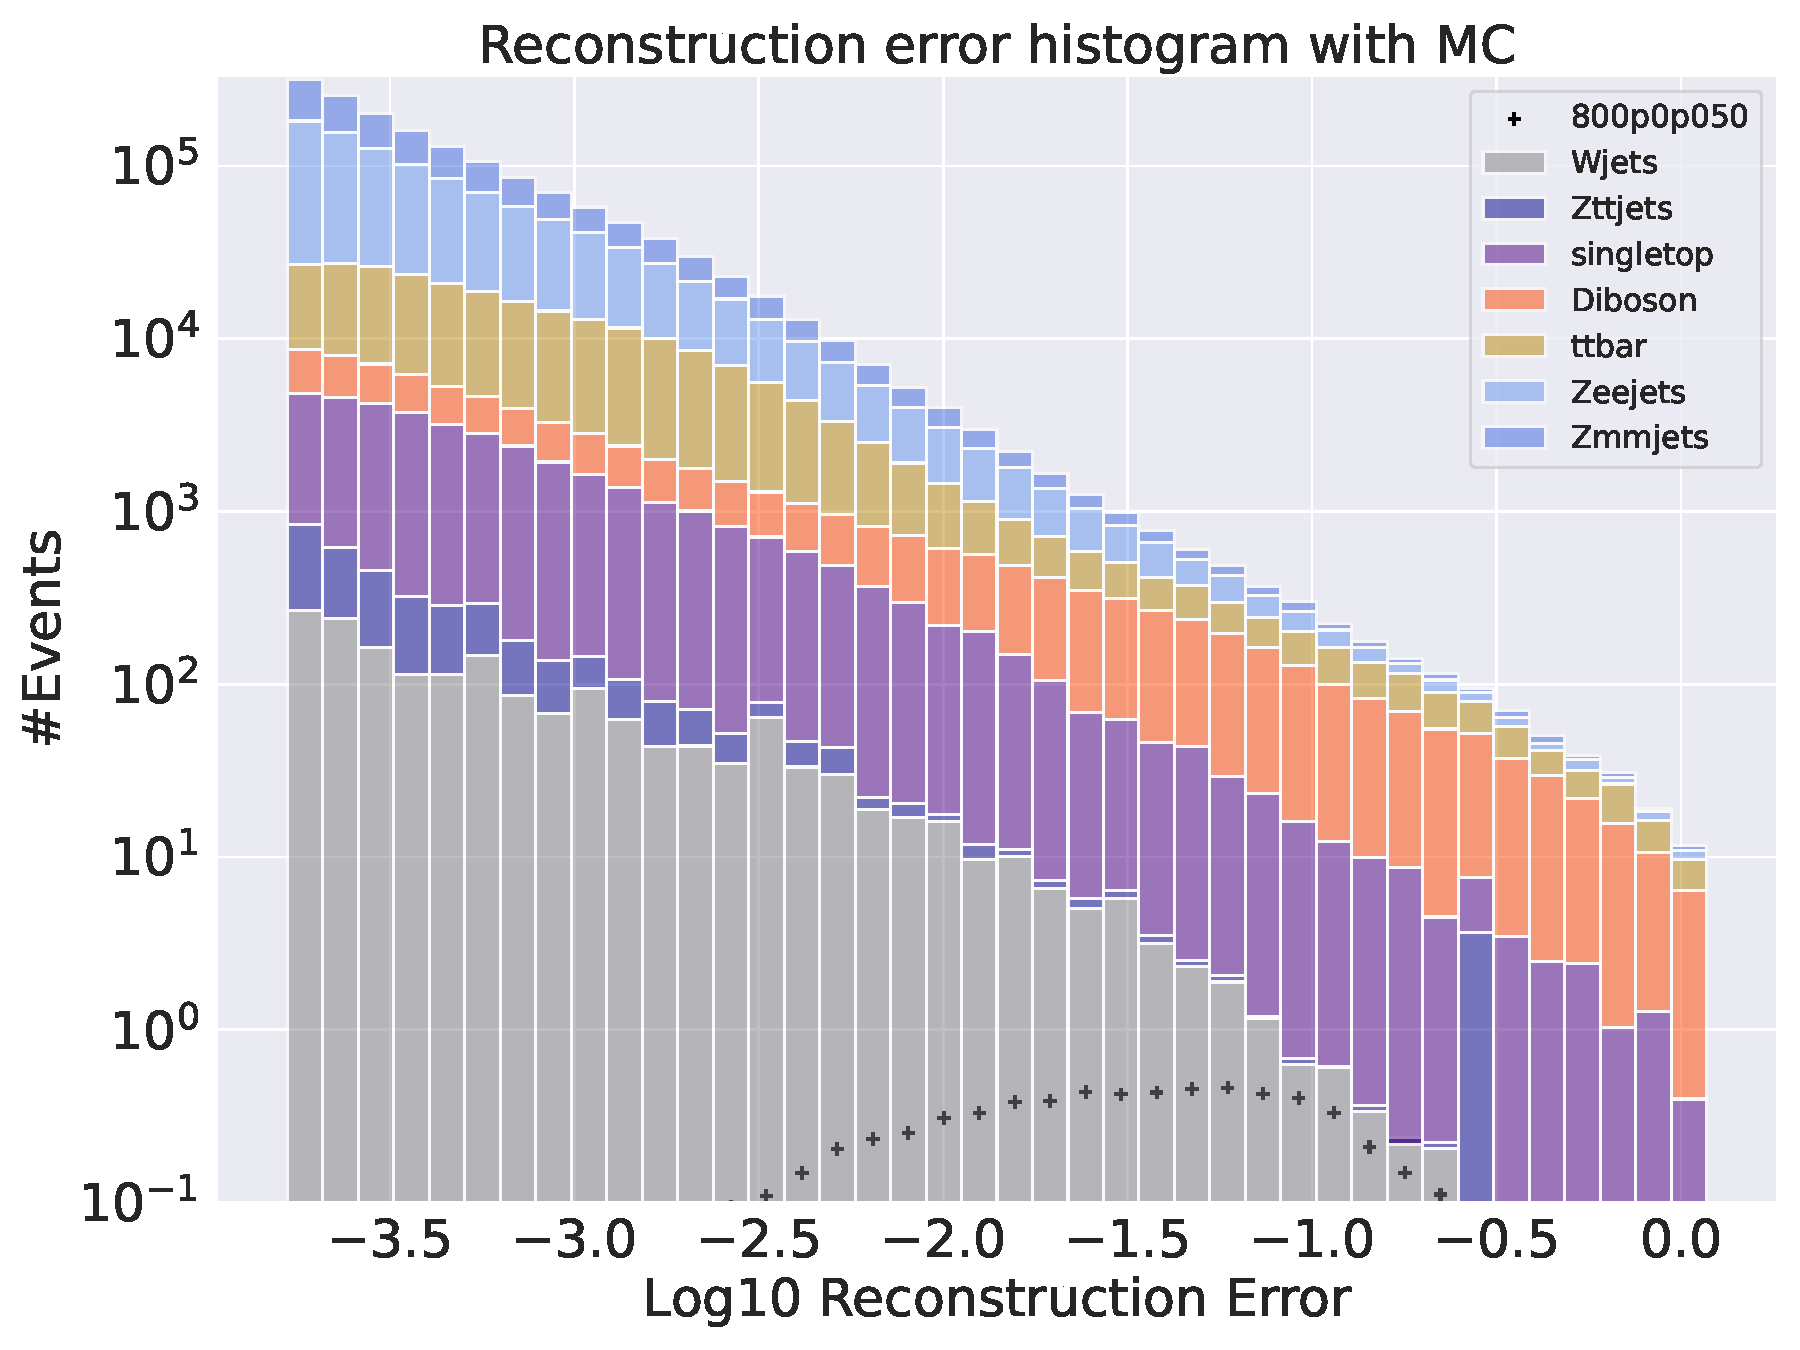
\includegraphics[width=\textwidth]{Figures/AE_testing/big/2lep/b_data_recon_big_rm3_feats_sig_800p0p050_.pdf}
        \caption{ }
        \label{fig:AE_2lep_big_800_3}
    \end{subfigure}
    \hfill
    \begin{subfigure}{.40\textwidth}
        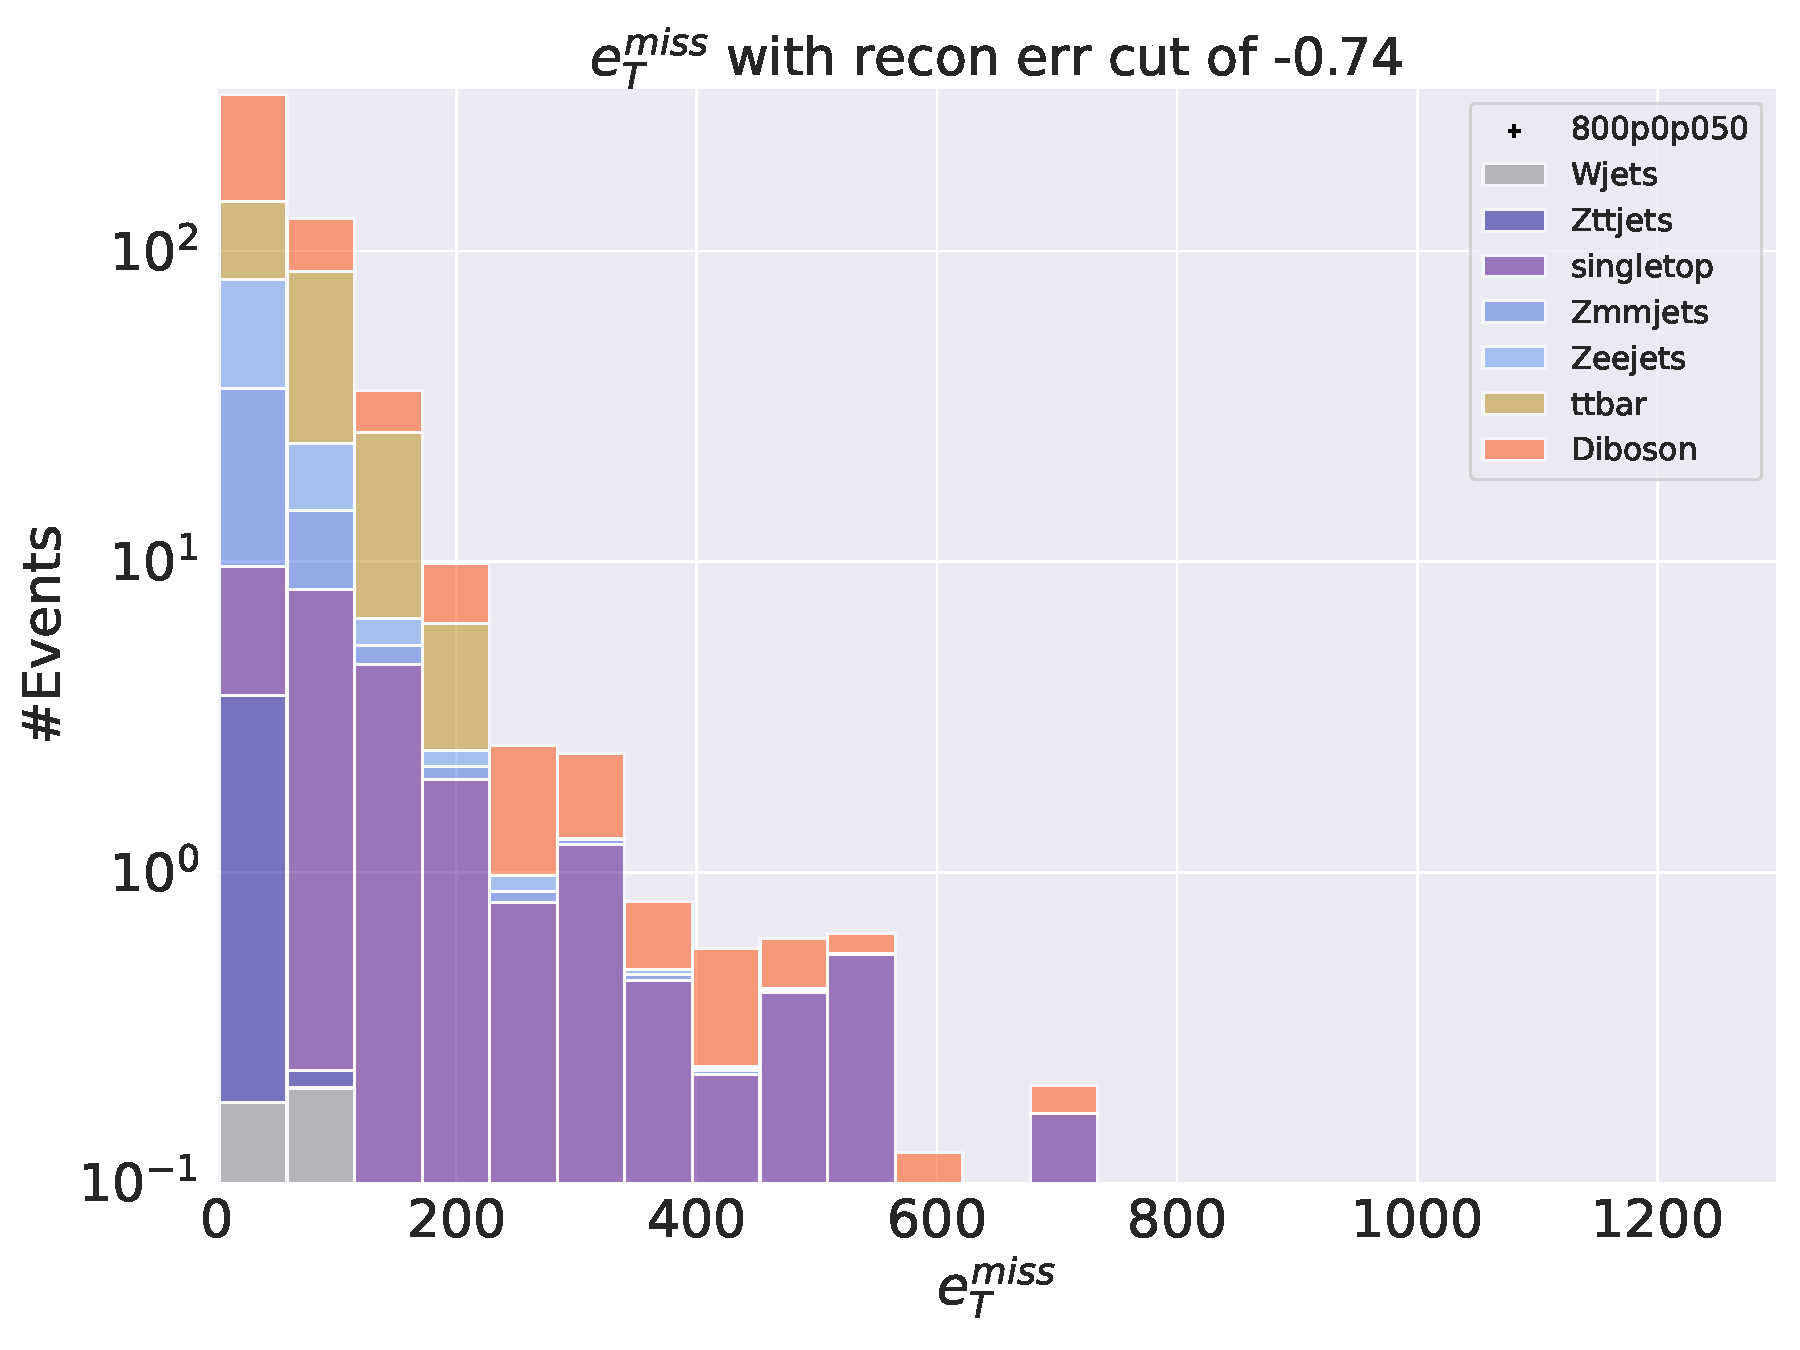
\includegraphics[width=\textwidth]{Figures/AE_testing/big/2lep/b_data_recon_big_rm3_feats_sig_800p0p050_recon_errcut_-0.74.pdf}
        \caption{}
        \label{fig:AE_2lep_big_etmiss_800_3}
    \end{subfigure}
    \hfill
      
    \begin{subfigure}{.40\textwidth}
        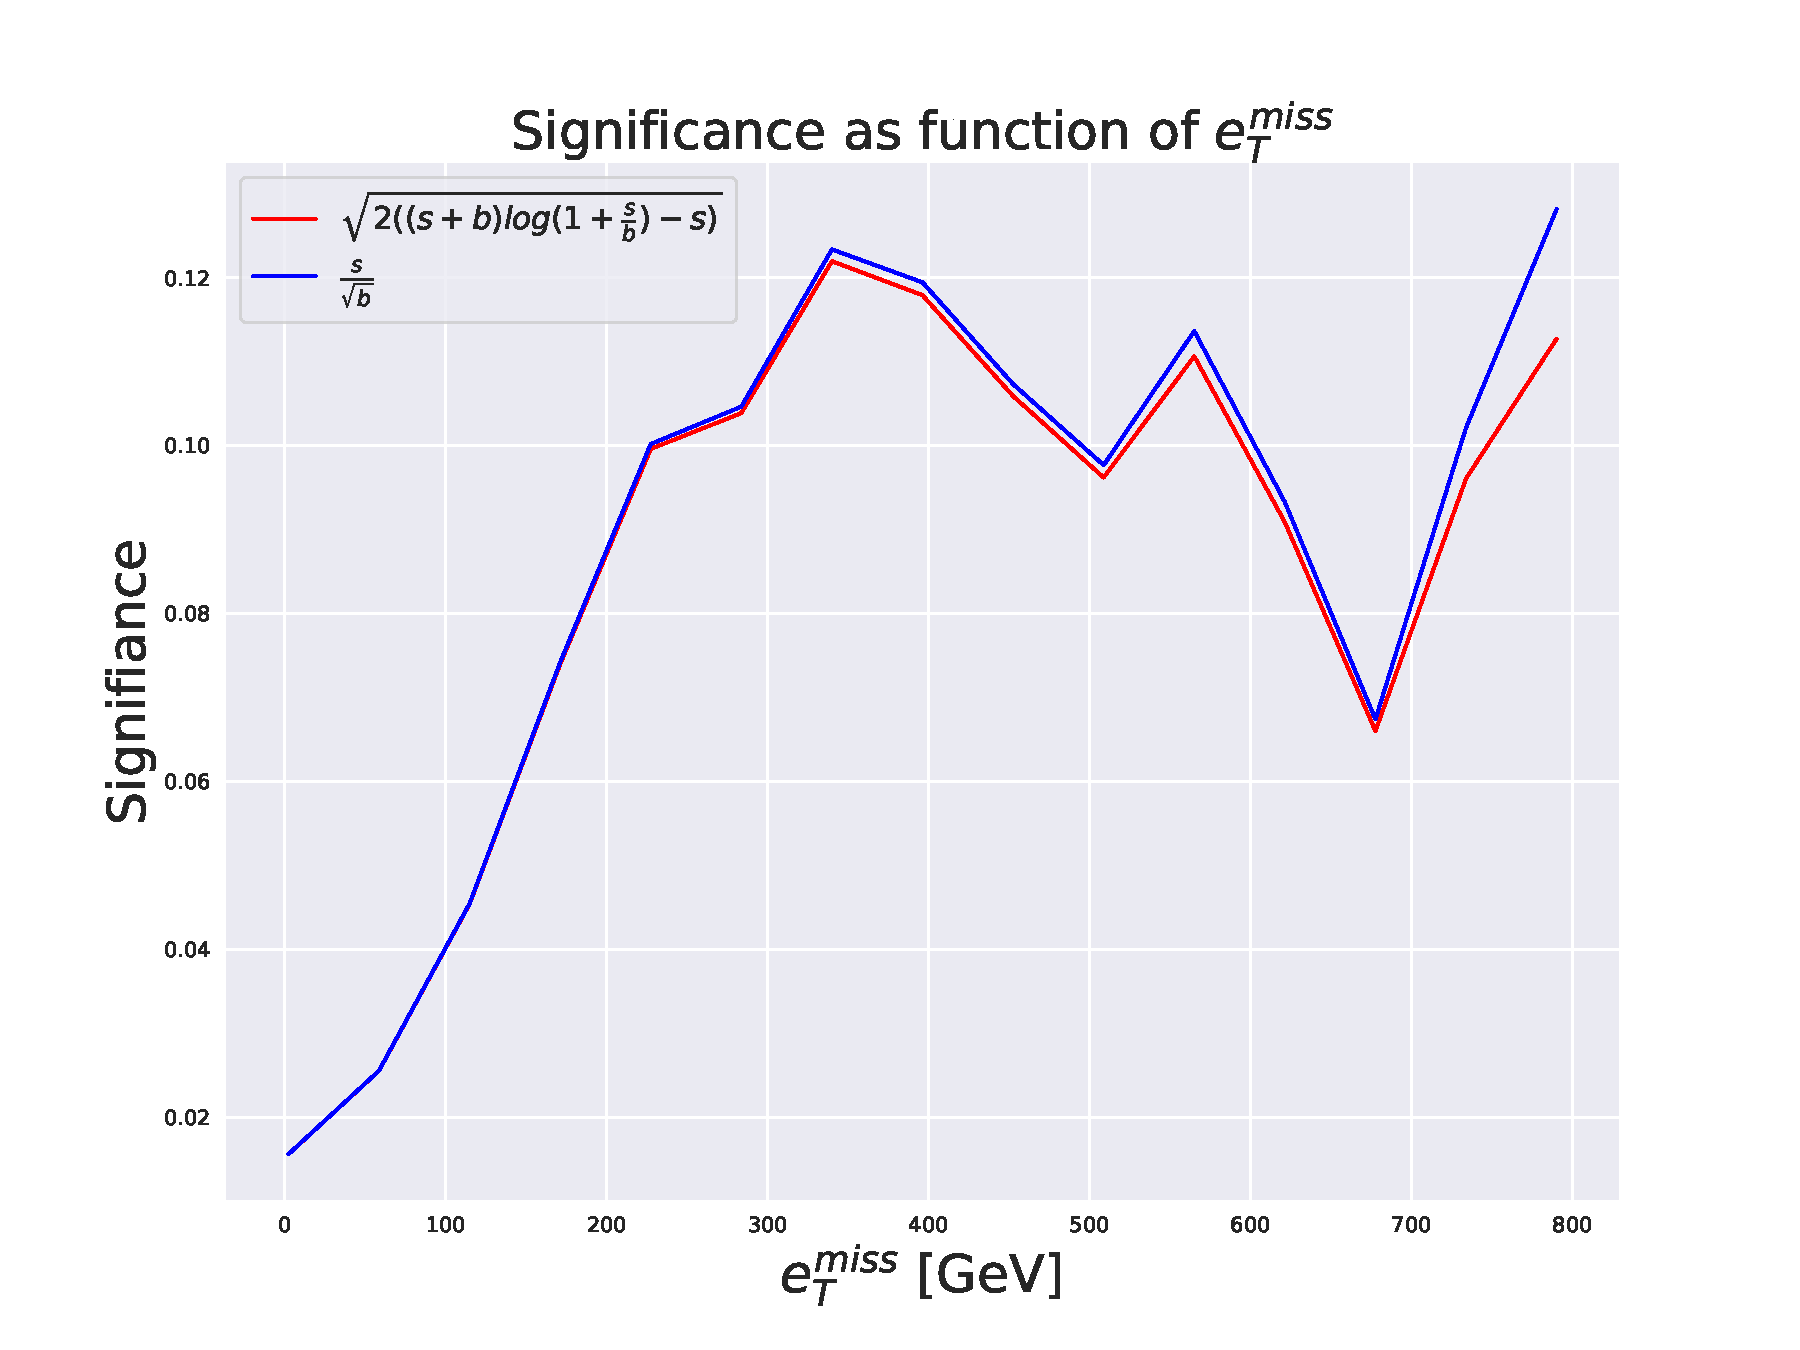
\includegraphics[width=\textwidth]{Figures/AE_testing/big/2lep/significance_etmiss_800p0p050_-0.7416855615358031.pdf}
        \caption{}
        \label{fig:AE_2lep_big_signi_800_3}
    \end{subfigure}
    \hfill      
    \caption[2lep deep network | $800p50$ | AE | 3]{Reconstruction error, $e_T^{miss}$ signal region, $m_{lll}$ signal region and significance as function of 
    $e_T^{miss}$ for the deep regular autoencoder. Here the SUSY $800p50$ model is used.}
    \label{fig:AE_2lep_big_rec_sig_signi_800_3}
\end{figure}

\begin{figure}[H]
    \centering
    \begin{subfigure}{.40\textwidth}
        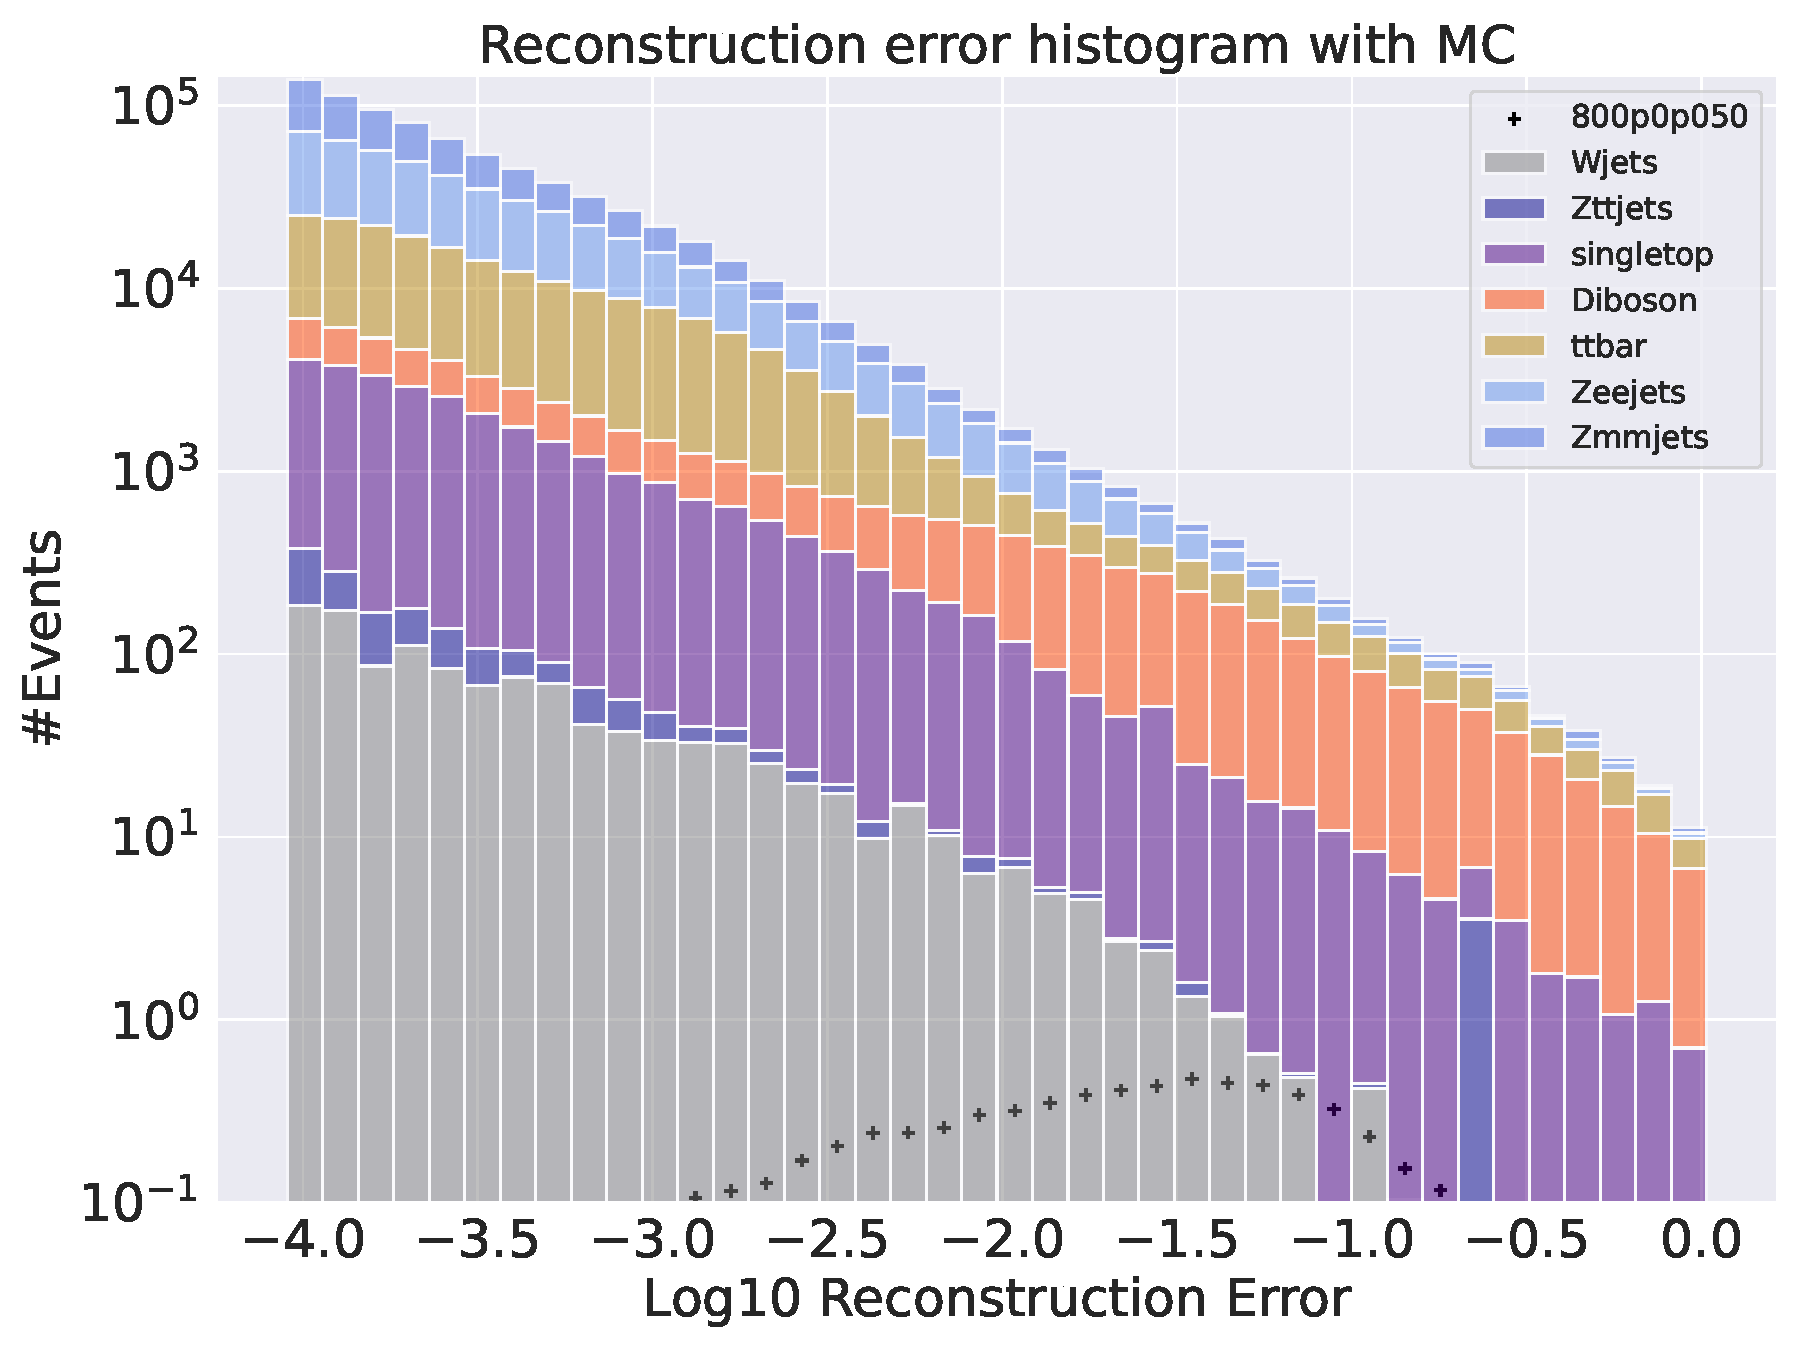
\includegraphics[width=\textwidth]{Figures/AE_testing/small/2lep/b_data_recon_big_rm3_feats_sig_800p0p050_.pdf}
        \caption{ }
        \label{fig:AE_2lep_small_800_3}
    \end{subfigure}
    \hfill
    \begin{subfigure}{.40\textwidth}
        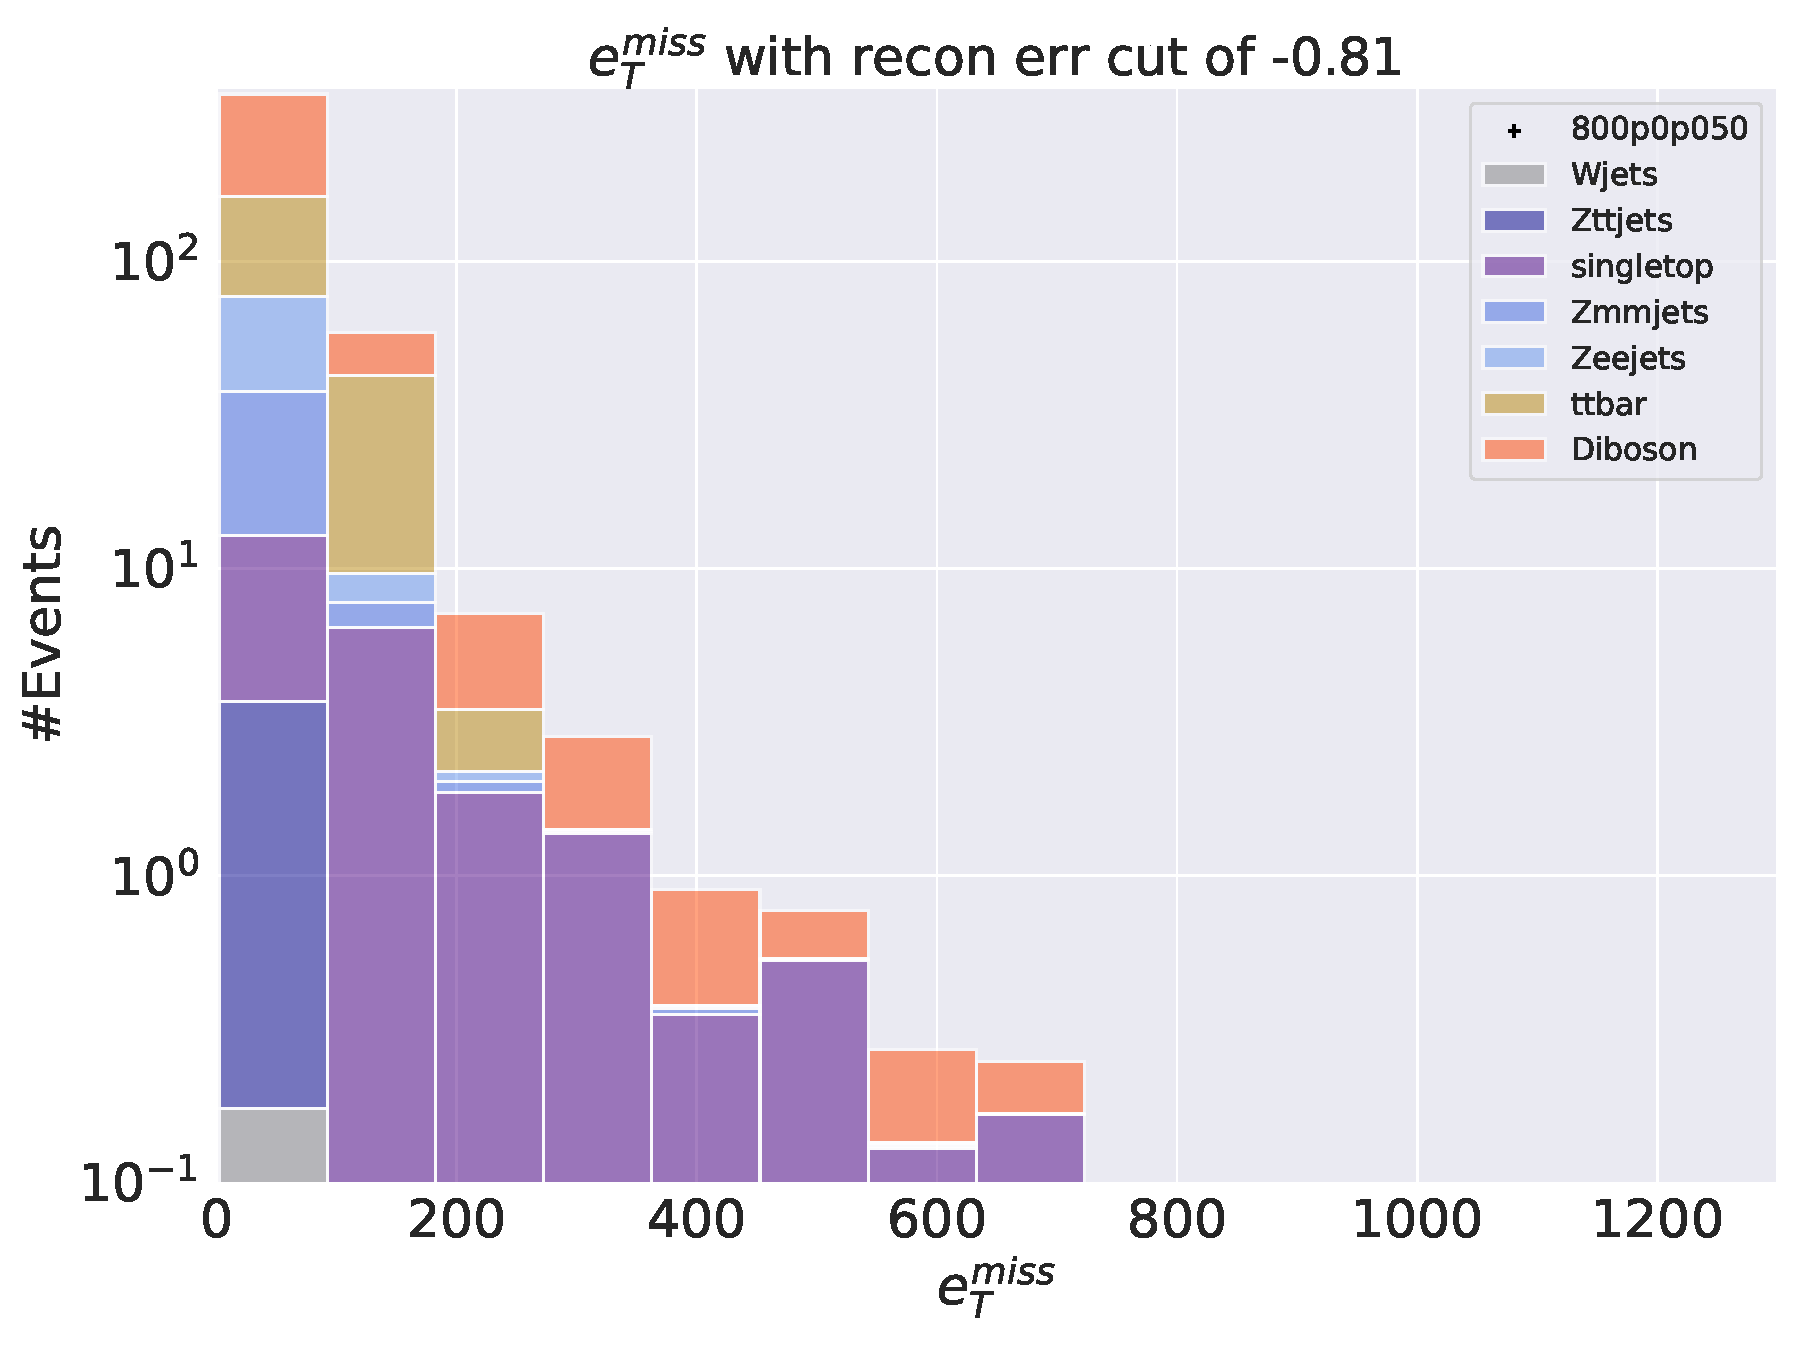
\includegraphics[width=\textwidth]{Figures/AE_testing/small/2lep/b_data_recon_big_rm3_feats_sig_800p0p050_recon_errcut_-0.81.pdf}
        \caption{}
        \label{fig:AE_2lep_small_etmiss_800_3}
    \end{subfigure}
    \hfill  
    \begin{subfigure}{.40\textwidth}
        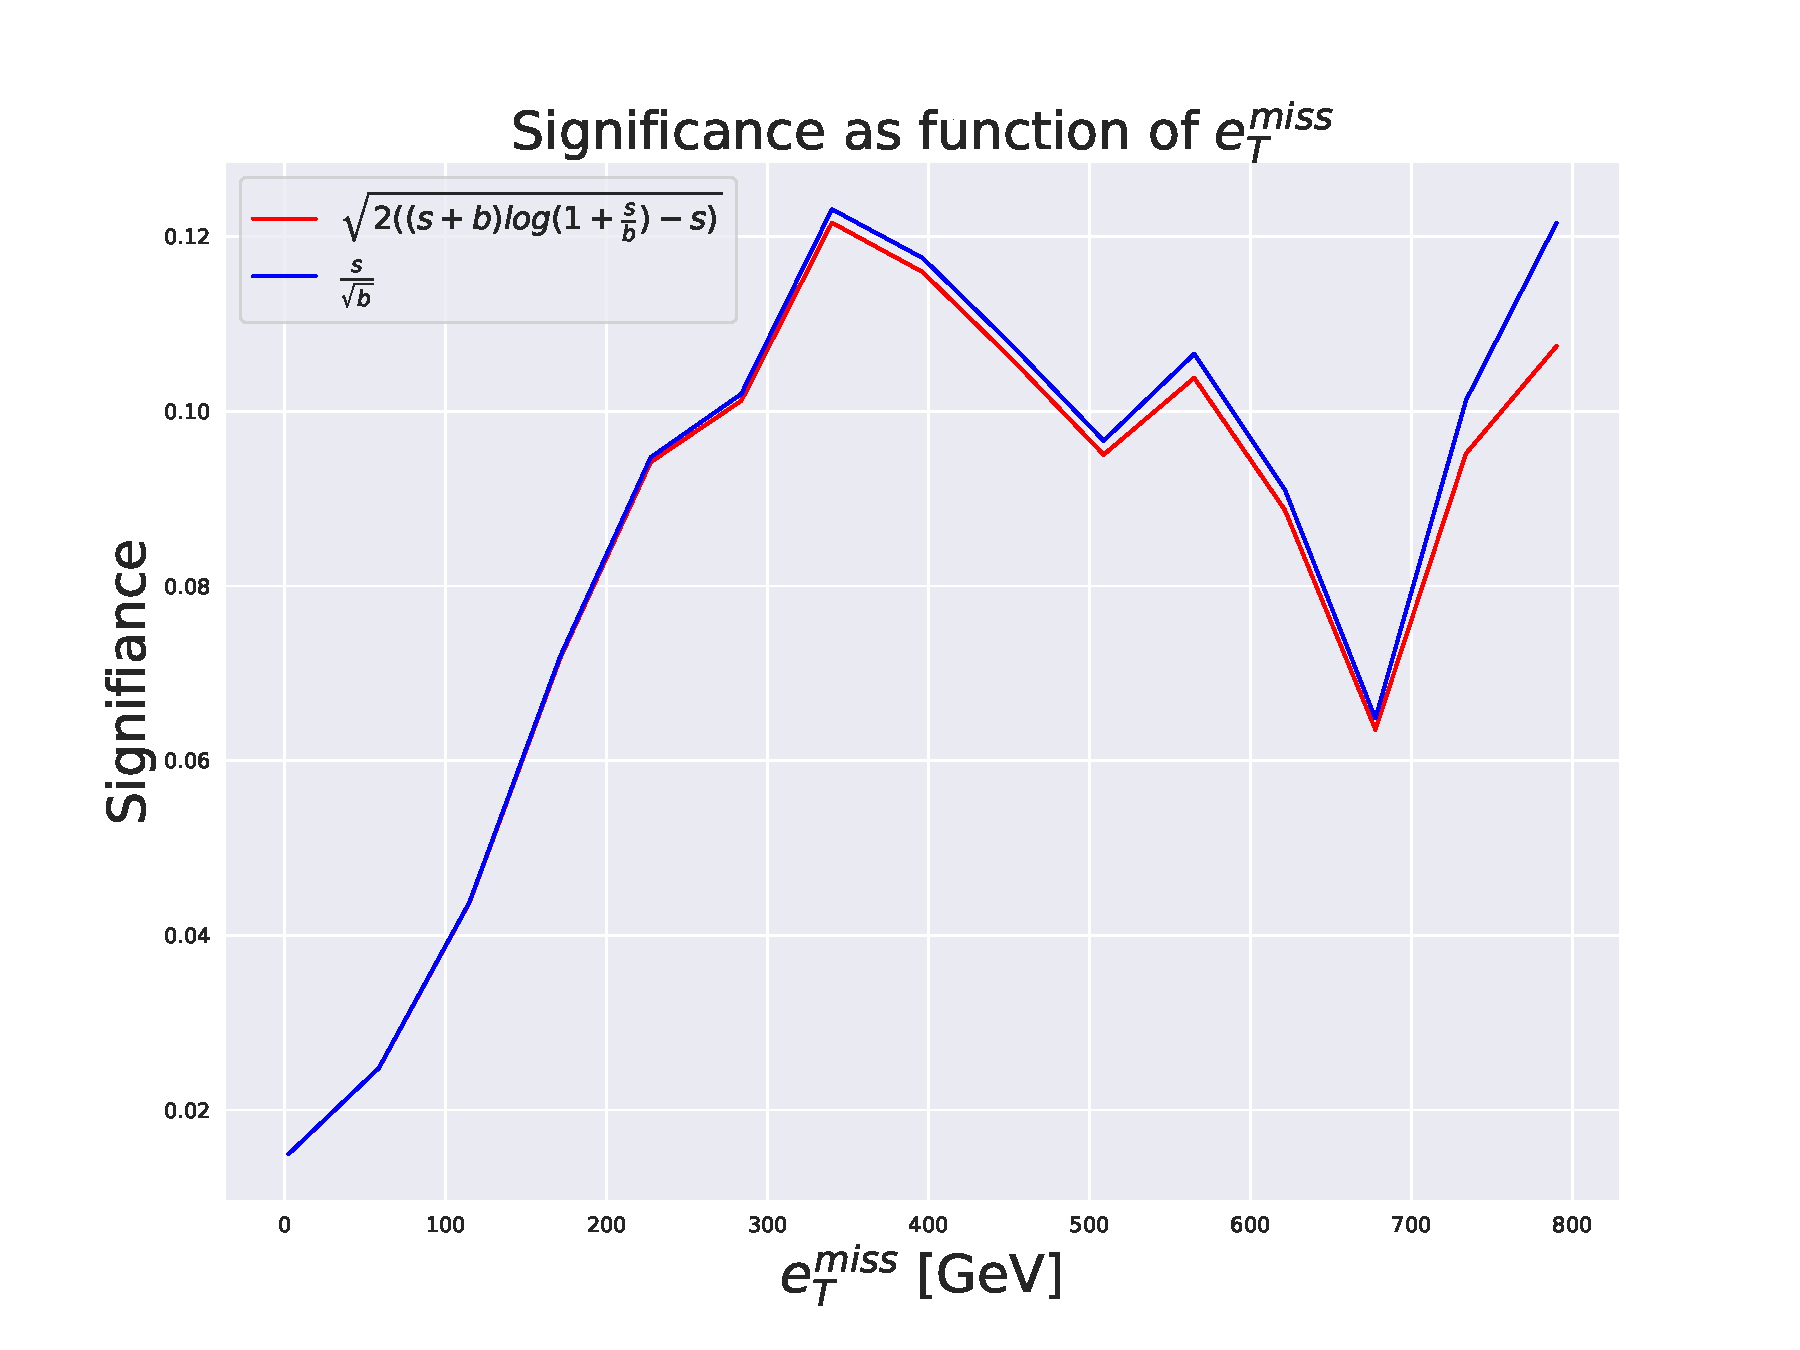
\includegraphics[width=\textwidth]{Figures/AE_testing/small/2lep/significance_etmiss_800p0p050_-0.805852780573614.pdf}
        \caption{}
        \label{fig:AE_2lep_small_signi_800_3}
    \end{subfigure}
    \hfill      
    \caption[2lep shallow network | $800p50$ | AE | 3]{Reconstruction error, $e_T^{miss}$ signal region, $m_{lll}$ signal region and significance as function of 
    $e_T^{miss}$ for the shallow regular autoencoder. Here the SUSY $800p50$ model is used.}
    \label{fig:AE_2lep_small_rec_sig_signi_800_3}
\end{figure}















\subsection*{Variational autoencoder output}












\begin{figure}[H]
    \centering
    \begin{subfigure}{.40\textwidth}
        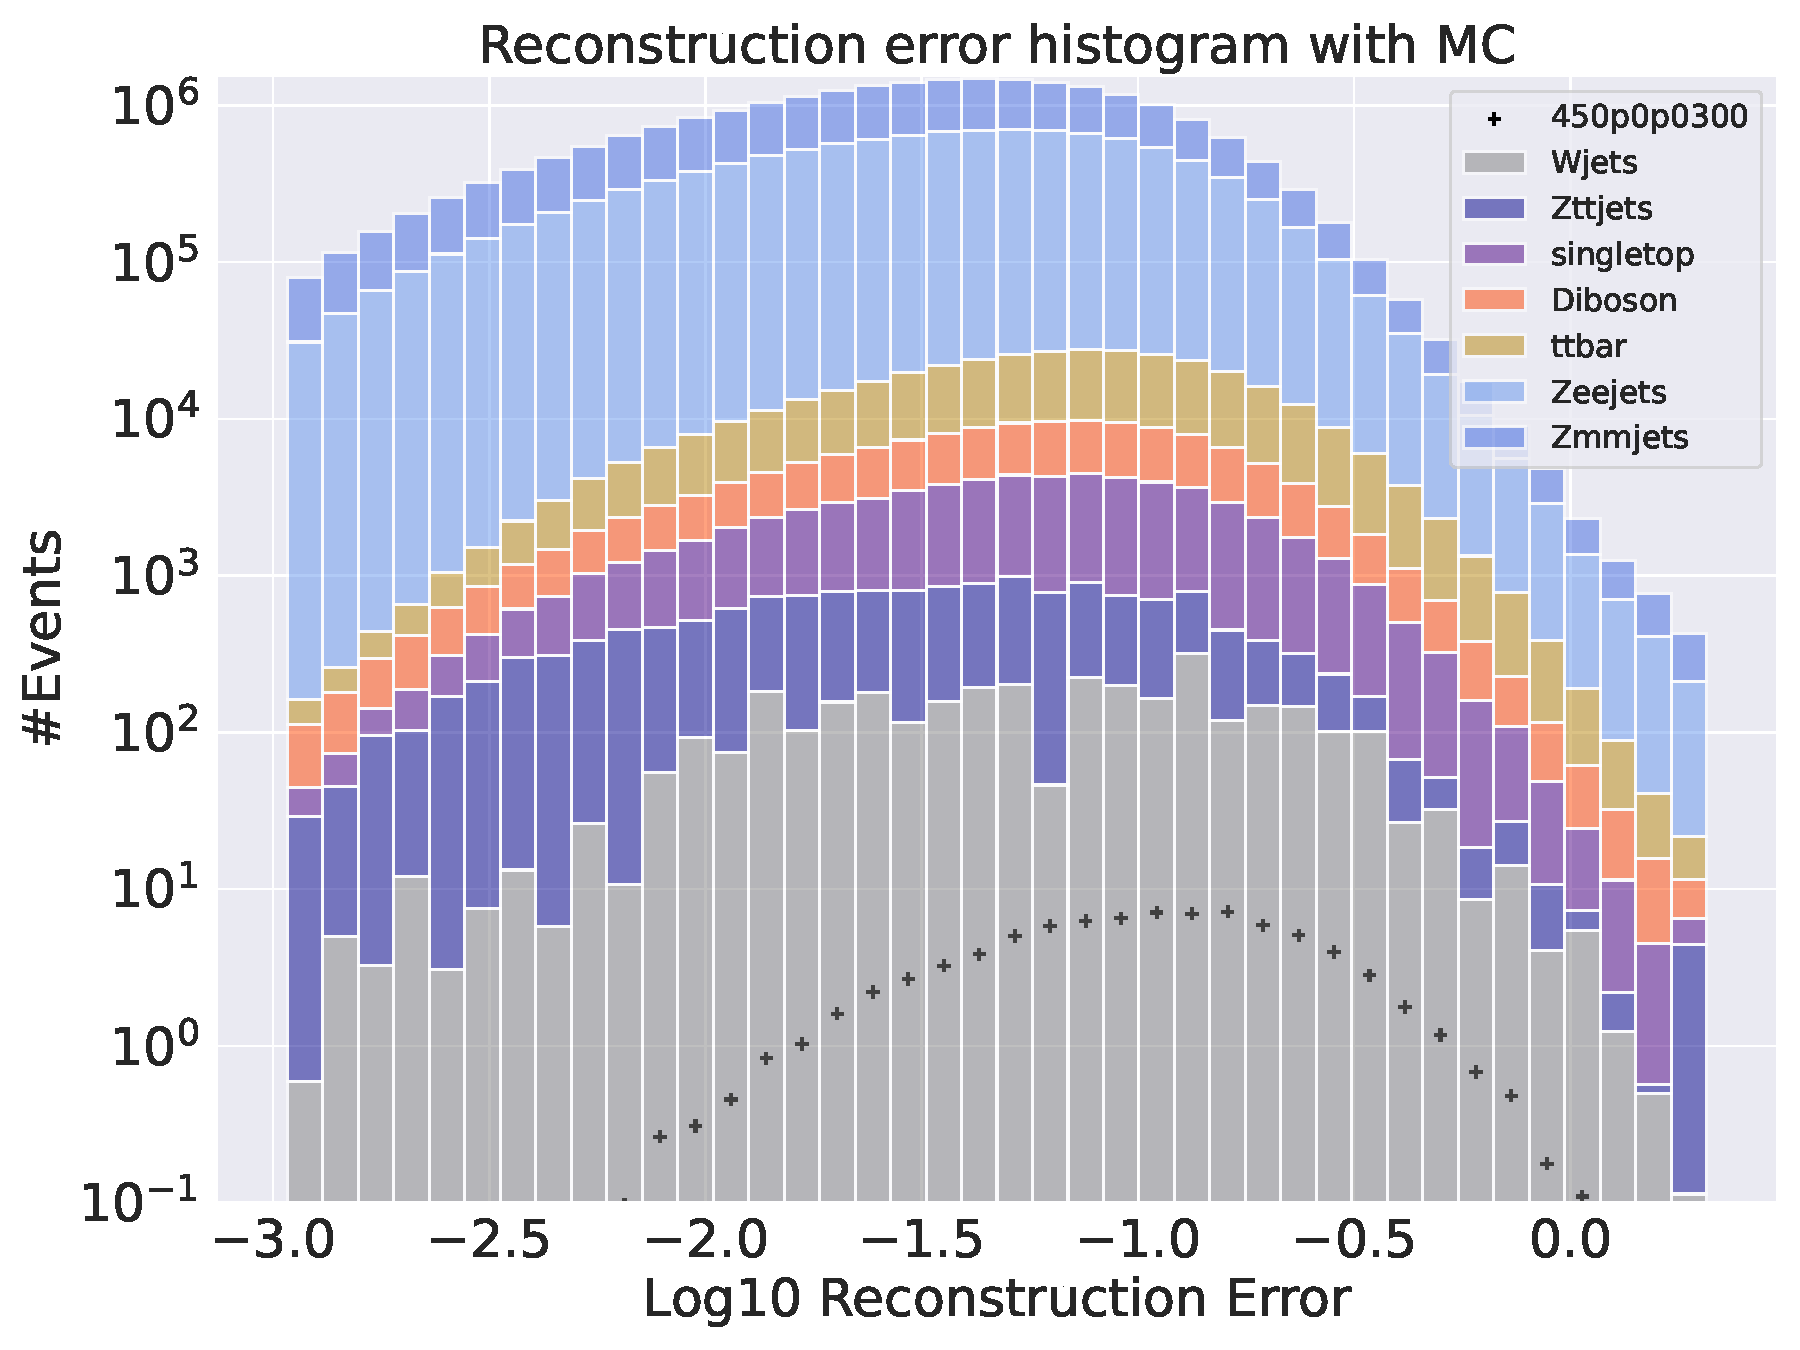
\includegraphics[width=\textwidth]{Figures/VAE_testing/small/2lep/b_data_recon_big_rm3_feats_sig_450p0p0300_.pdf}
        \caption{ }
        \label{fig:VAE_2lep_big_450_2}
    \end{subfigure}
    \hfill
    \begin{subfigure}{.40\textwidth}
        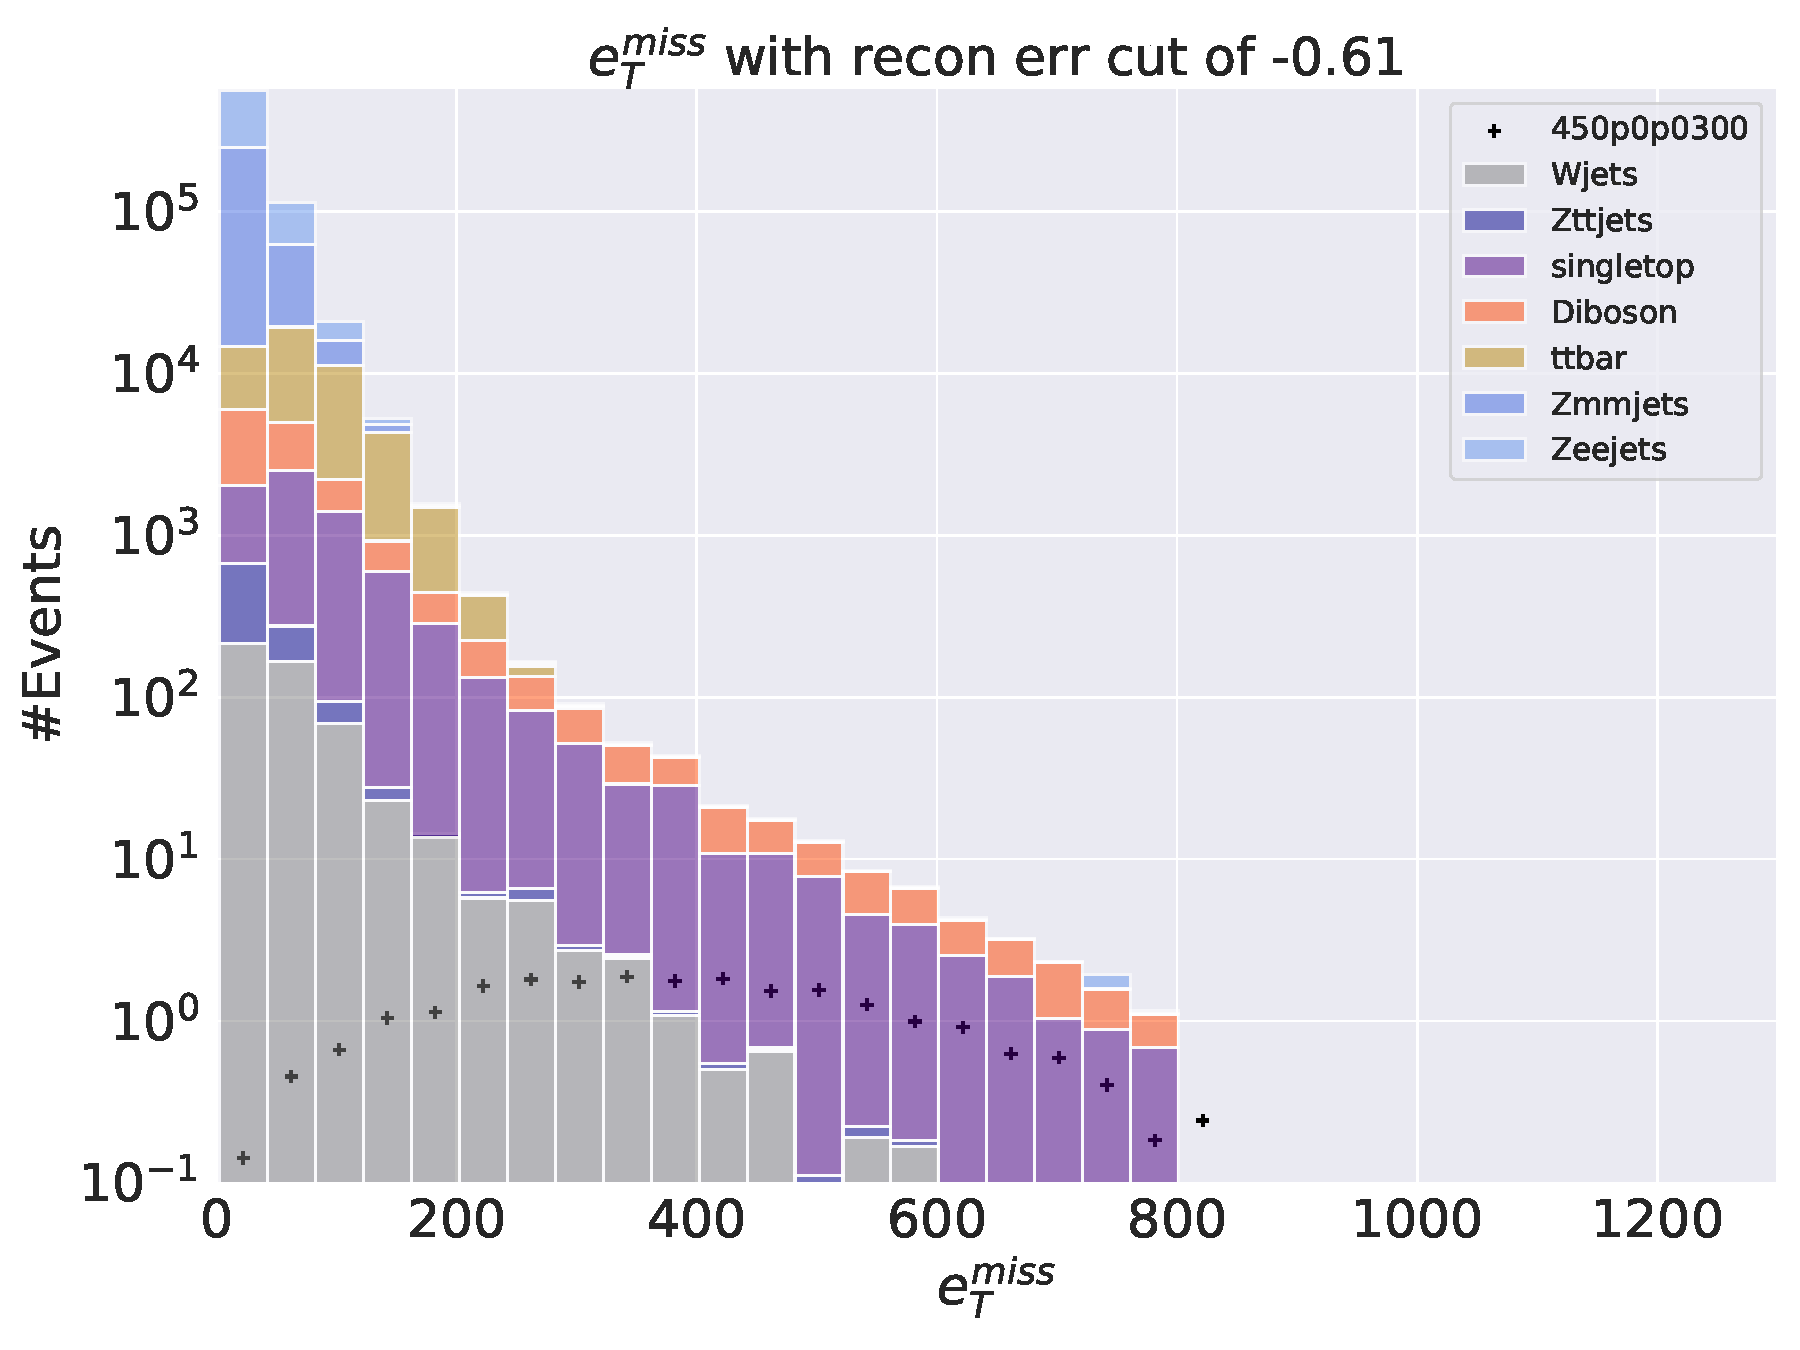
\includegraphics[width=\textwidth]{Figures/VAE_testing/big/2lep/b_data_recon_big_rm3_feats_sig_450p0p0300_recon_errcut_-0.61.pdf}
        \caption{}
        \label{fig:VAE_2lep_big_etmiss_450_2}
    \end{subfigure}
    \hfill 
    \begin{subfigure}{.40\textwidth}
        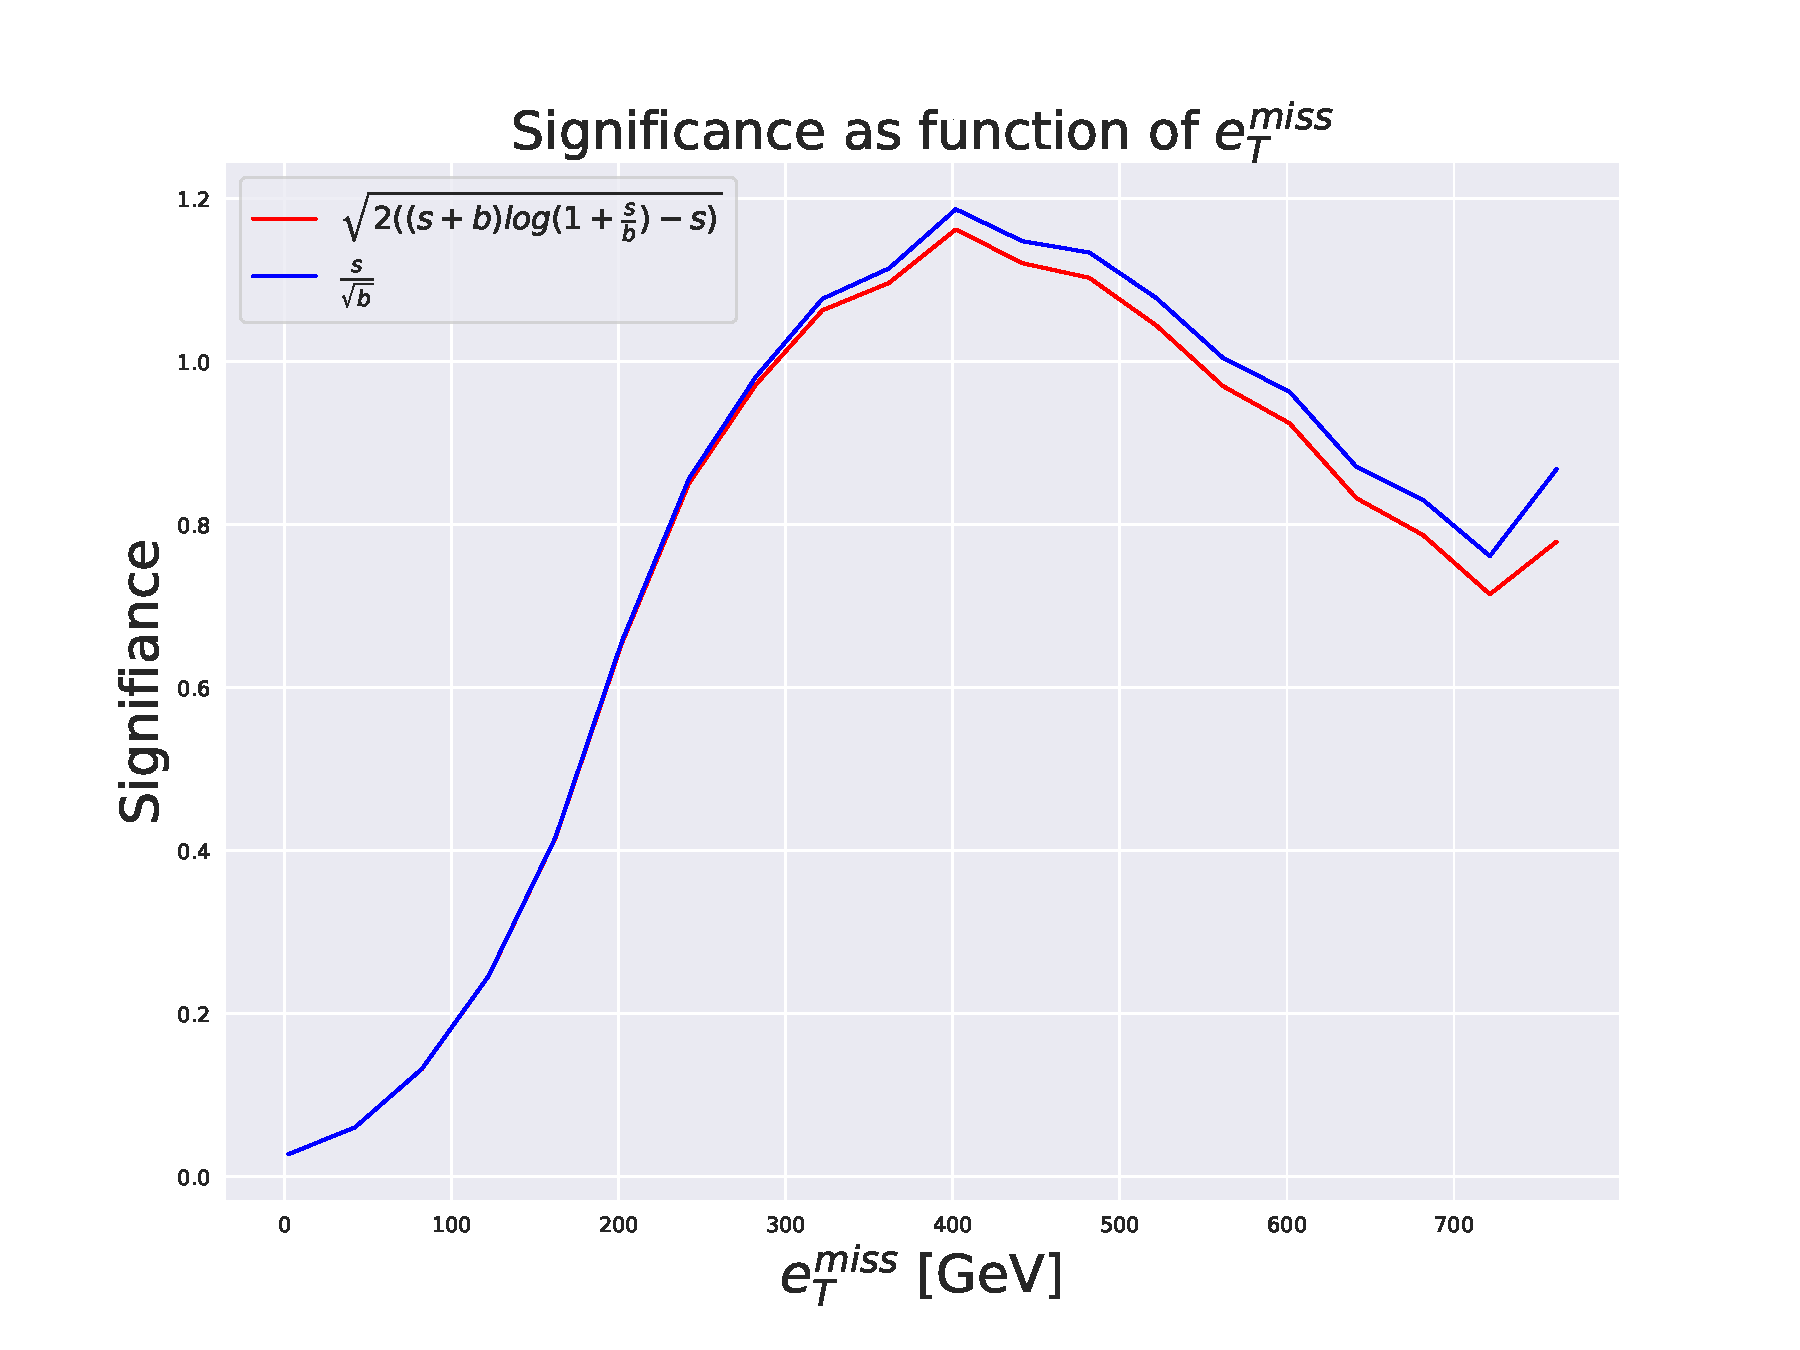
\includegraphics[width=\textwidth]{Figures/VAE_testing/big/2lep/significance_etmiss_450p0p0300_-0.6091405575830948.pdf}
        \caption{}
        \label{fig:VAE_2lep_big_signi_450_2}
    \end{subfigure}
    \hfill      
    \caption[2lep deep network | $450p300$ | VAE | 2]{Reconstruction error, $e_T^{miss}$ signal region, $m_{lll}$ signal region and significance as function of 
    $e_T^{miss}$ for the deep regular autoencoder. Here the SUSY $450p300$ model is used.}
    \label{fig:VAE_2lep_big_rec_sig_signi_450_2}
\end{figure}

\begin{figure}[H]
    \centering
    \begin{subfigure}{.40\textwidth}
        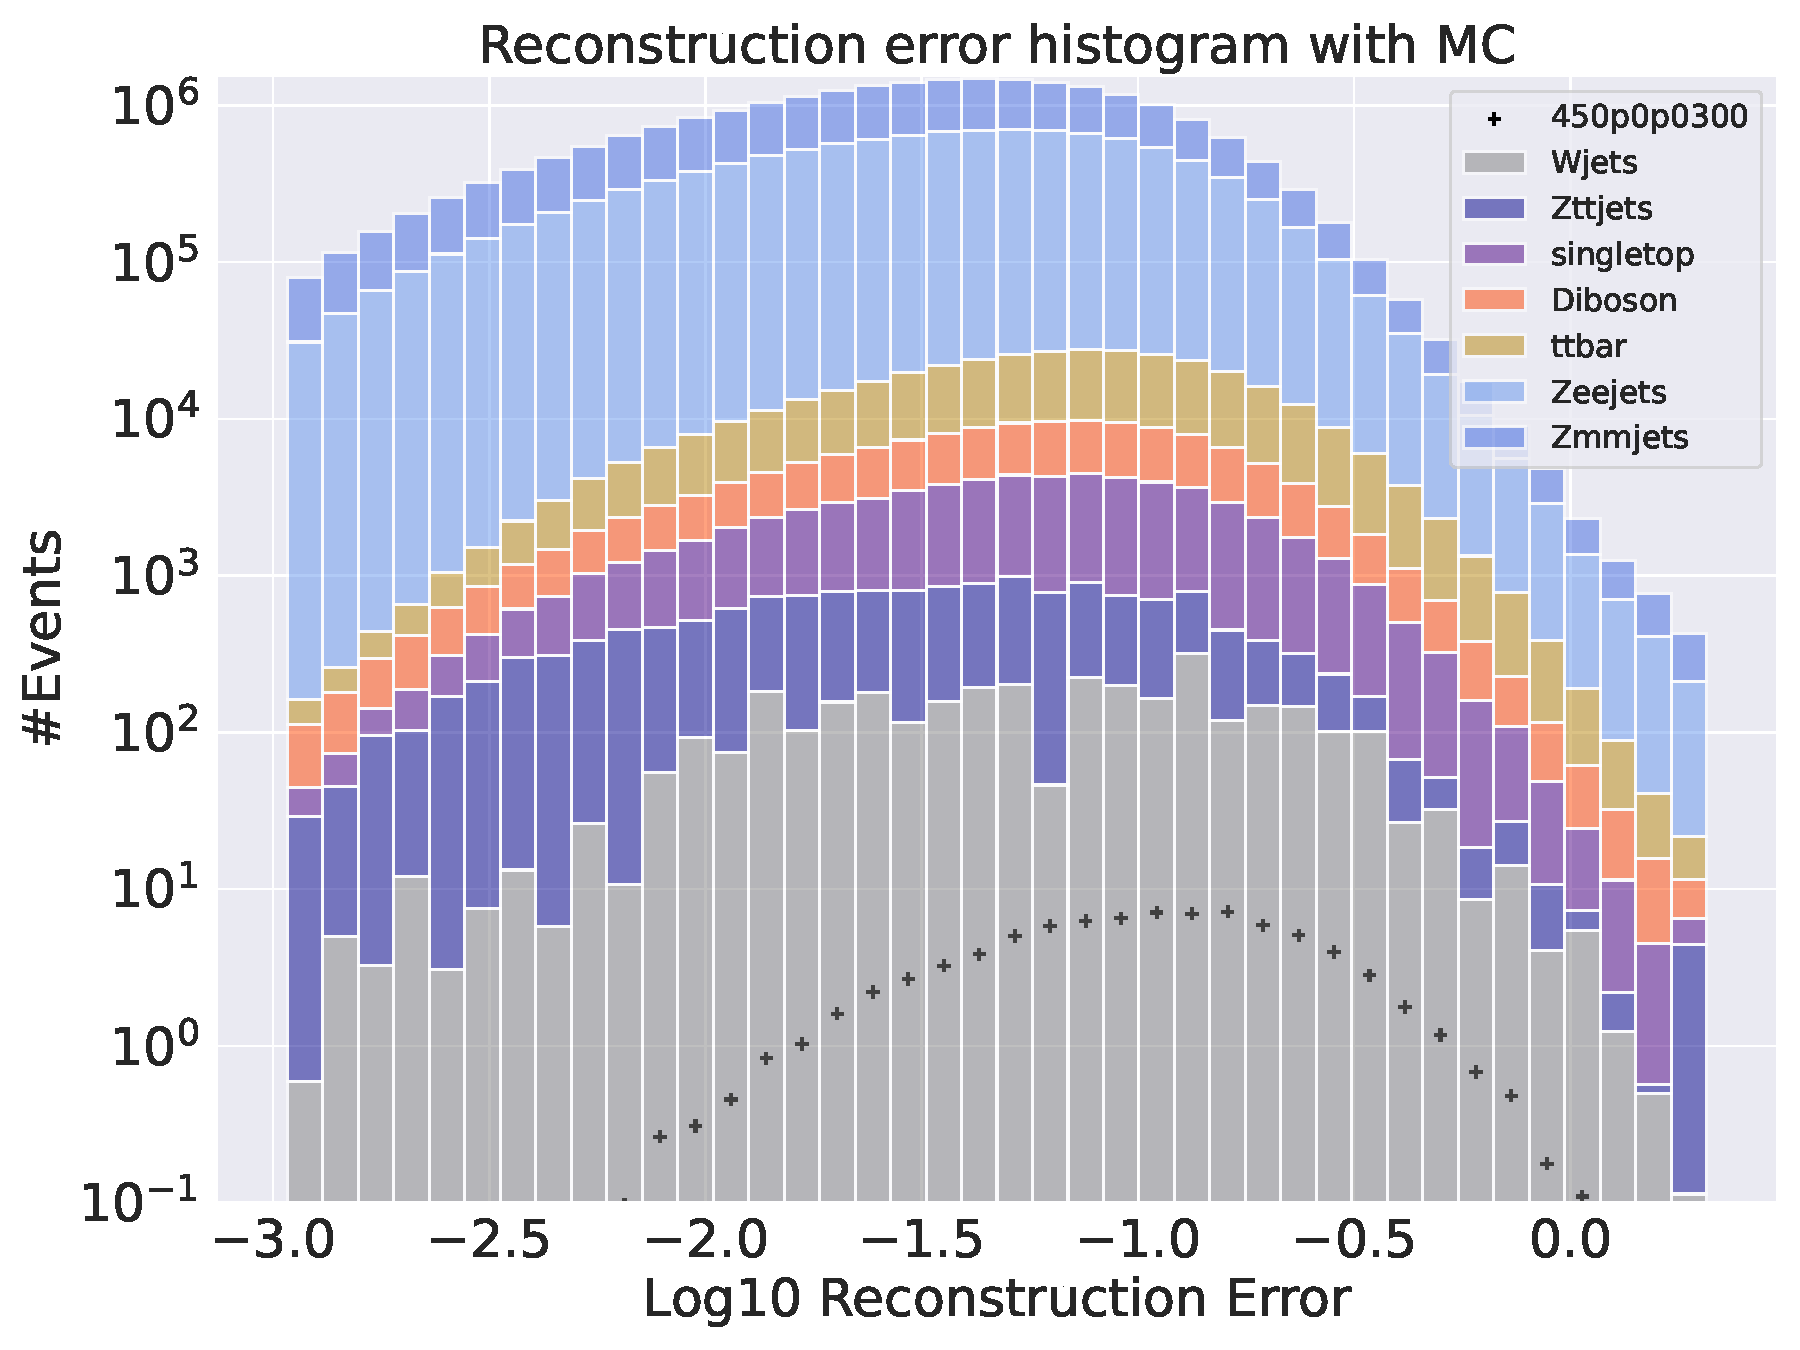
\includegraphics[width=\textwidth]{Figures/VAE_testing/small/2lep/b_data_recon_big_rm3_feats_sig_450p0p0300_.pdf}
        \caption{ }
        \label{fig:VAE_2lep_small_450_2}
    \end{subfigure}
    \hfill
    \begin{subfigure}{.40\textwidth}
        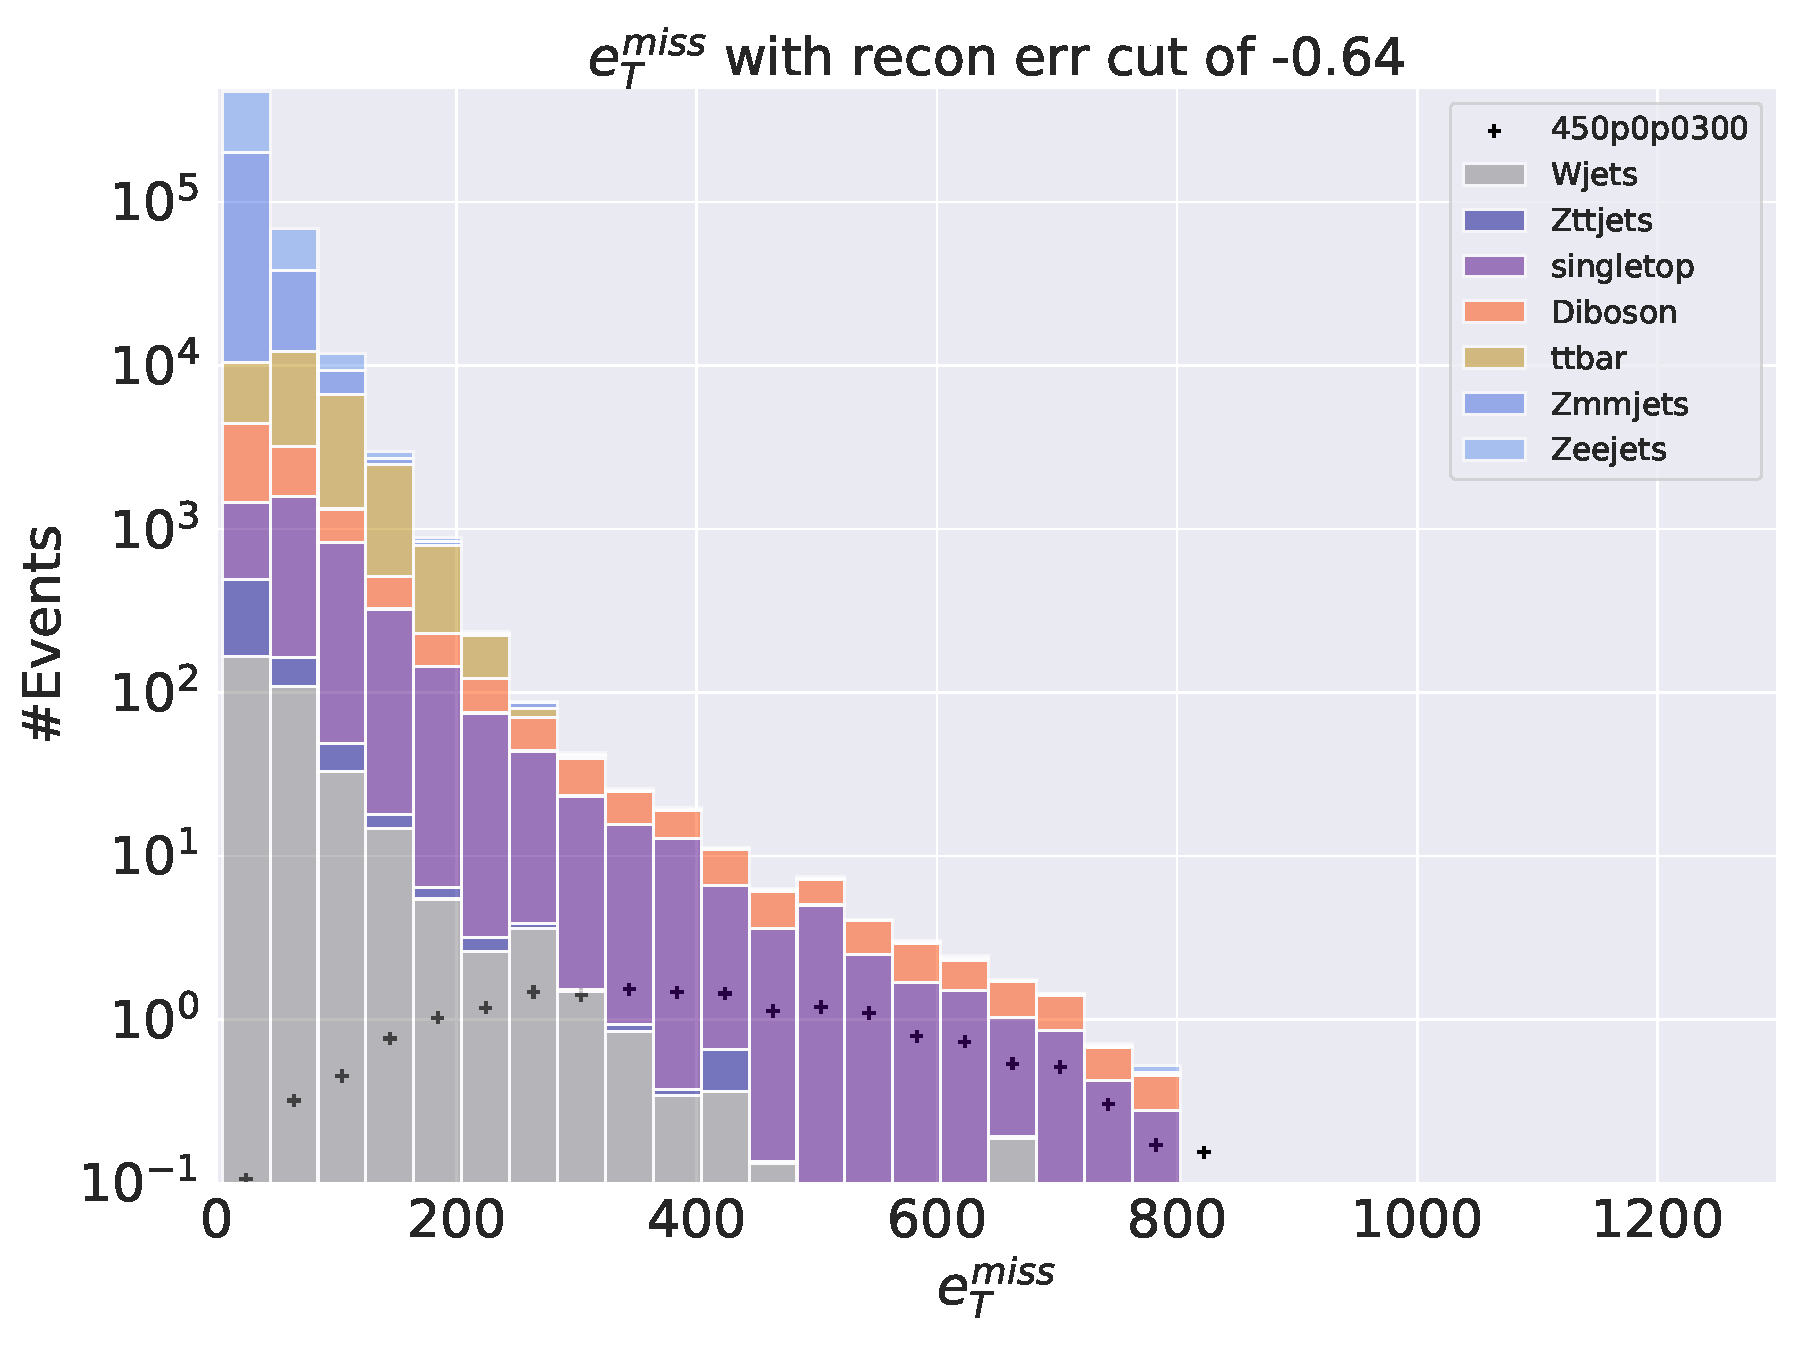
\includegraphics[width=\textwidth]{Figures/VAE_testing/small/2lep/b_data_recon_big_rm3_feats_sig_450p0p0300_recon_errcut_-0.64.pdf}
        \caption{}
        \label{fig:VAE_2lep_small_etmiss_450_2}
    \end{subfigure}
    \hfill  
    \begin{subfigure}{.40\textwidth}
        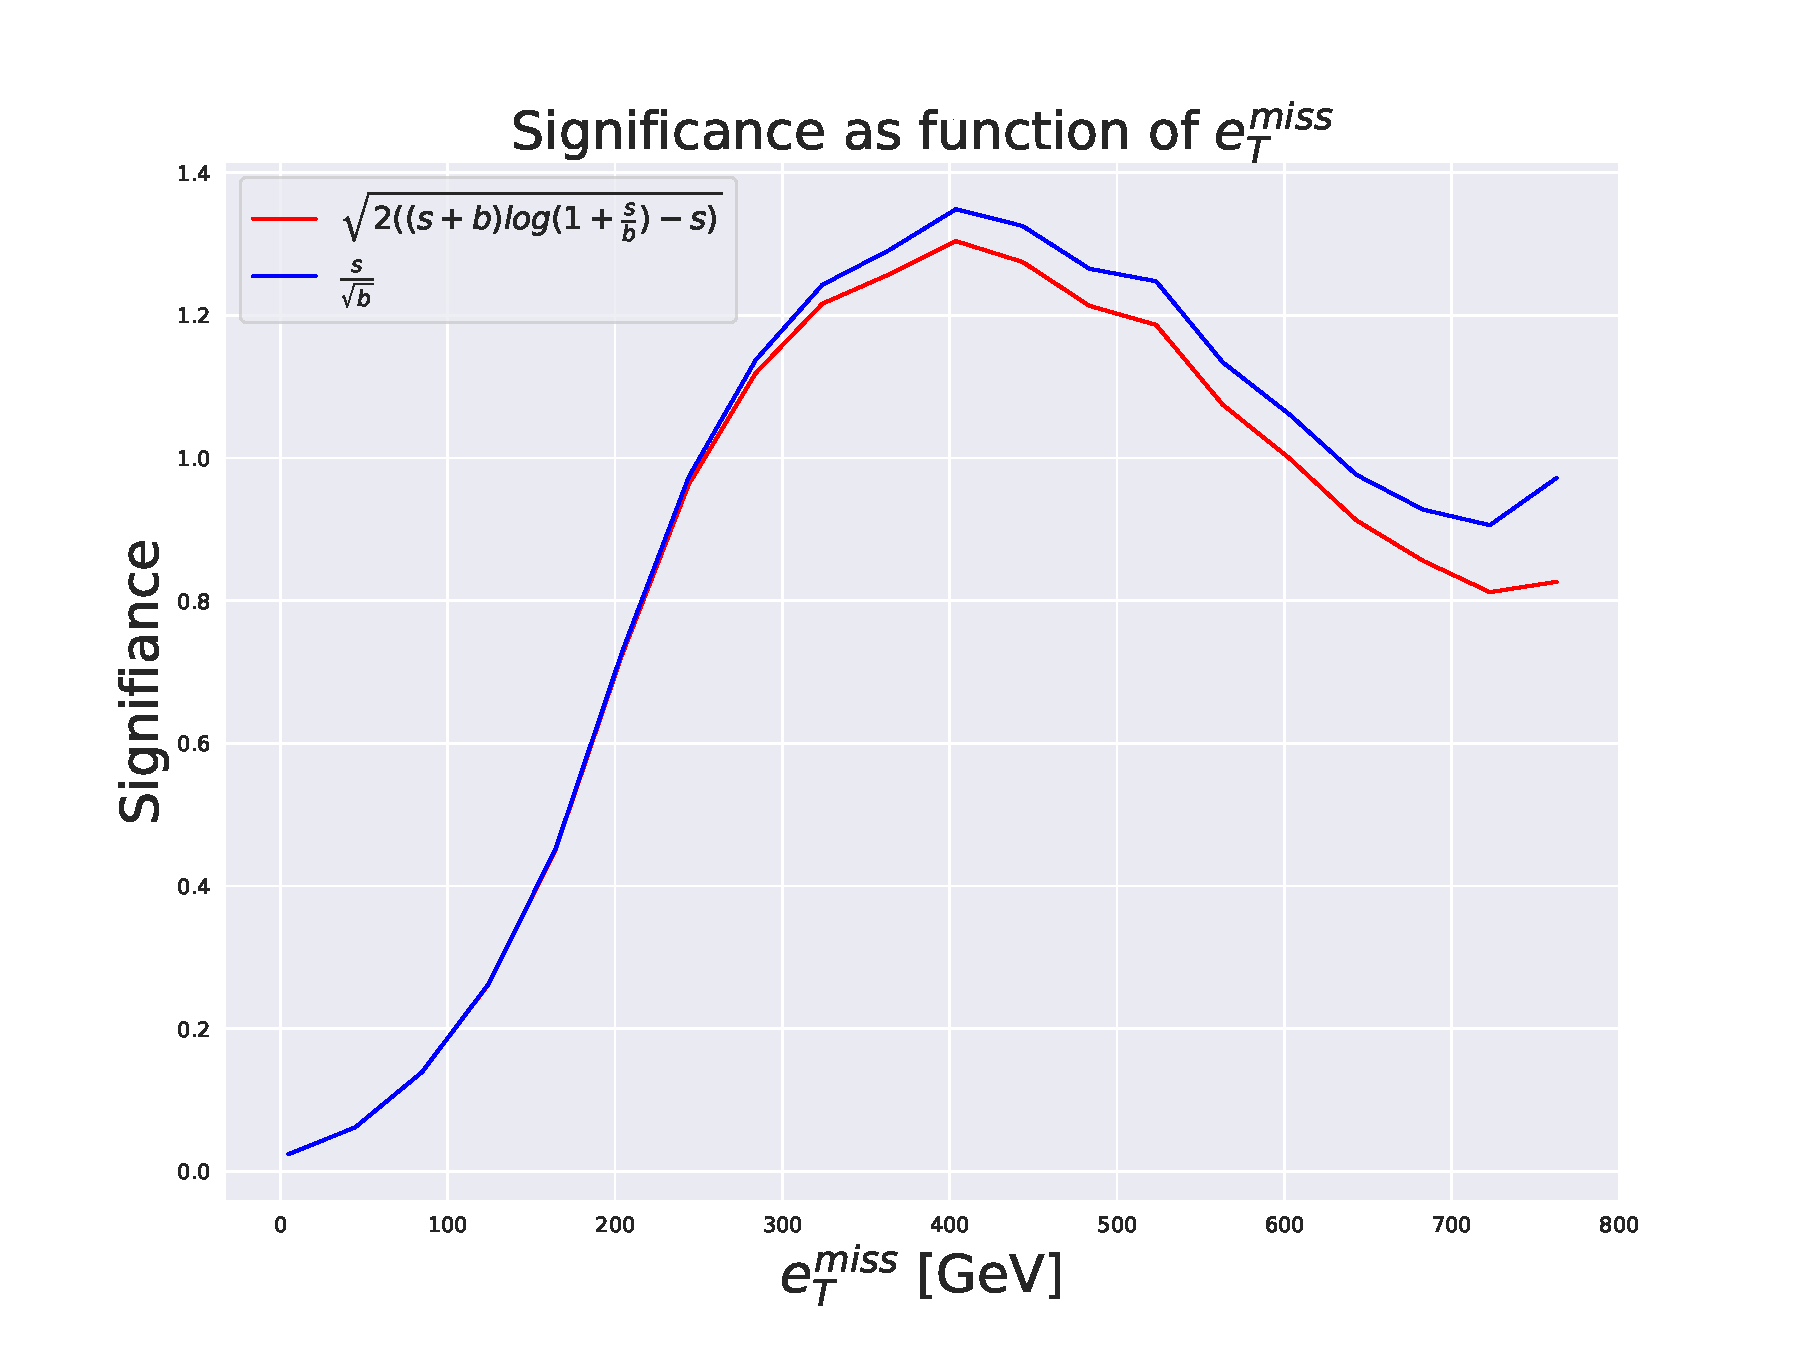
\includegraphics[width=\textwidth]{Figures/VAE_testing/small/2lep/significance_etmiss_450p0p0300_-0.6363602624727392.pdf}
        \caption{}
        \label{fig:VAE_2lep_small_signi_450_2}
    \end{subfigure}
    \hfill      
    \caption[2lep shallow network | $450p300$ | VAE | 2]{Reconstruction error, $e_T^{miss}$ signal region, $m_{lll}$ signal region and significance as function of 
    $e_T^{miss}$ for the deep regular autoencoder. Here the SUSY $450p300$ model is used.}
    \label{fig:VAE_2lep_small_rec_sig_signi_450_2}
\end{figure}


\begin{figure}[H]
    \centering
    \begin{subfigure}{.40\textwidth}
        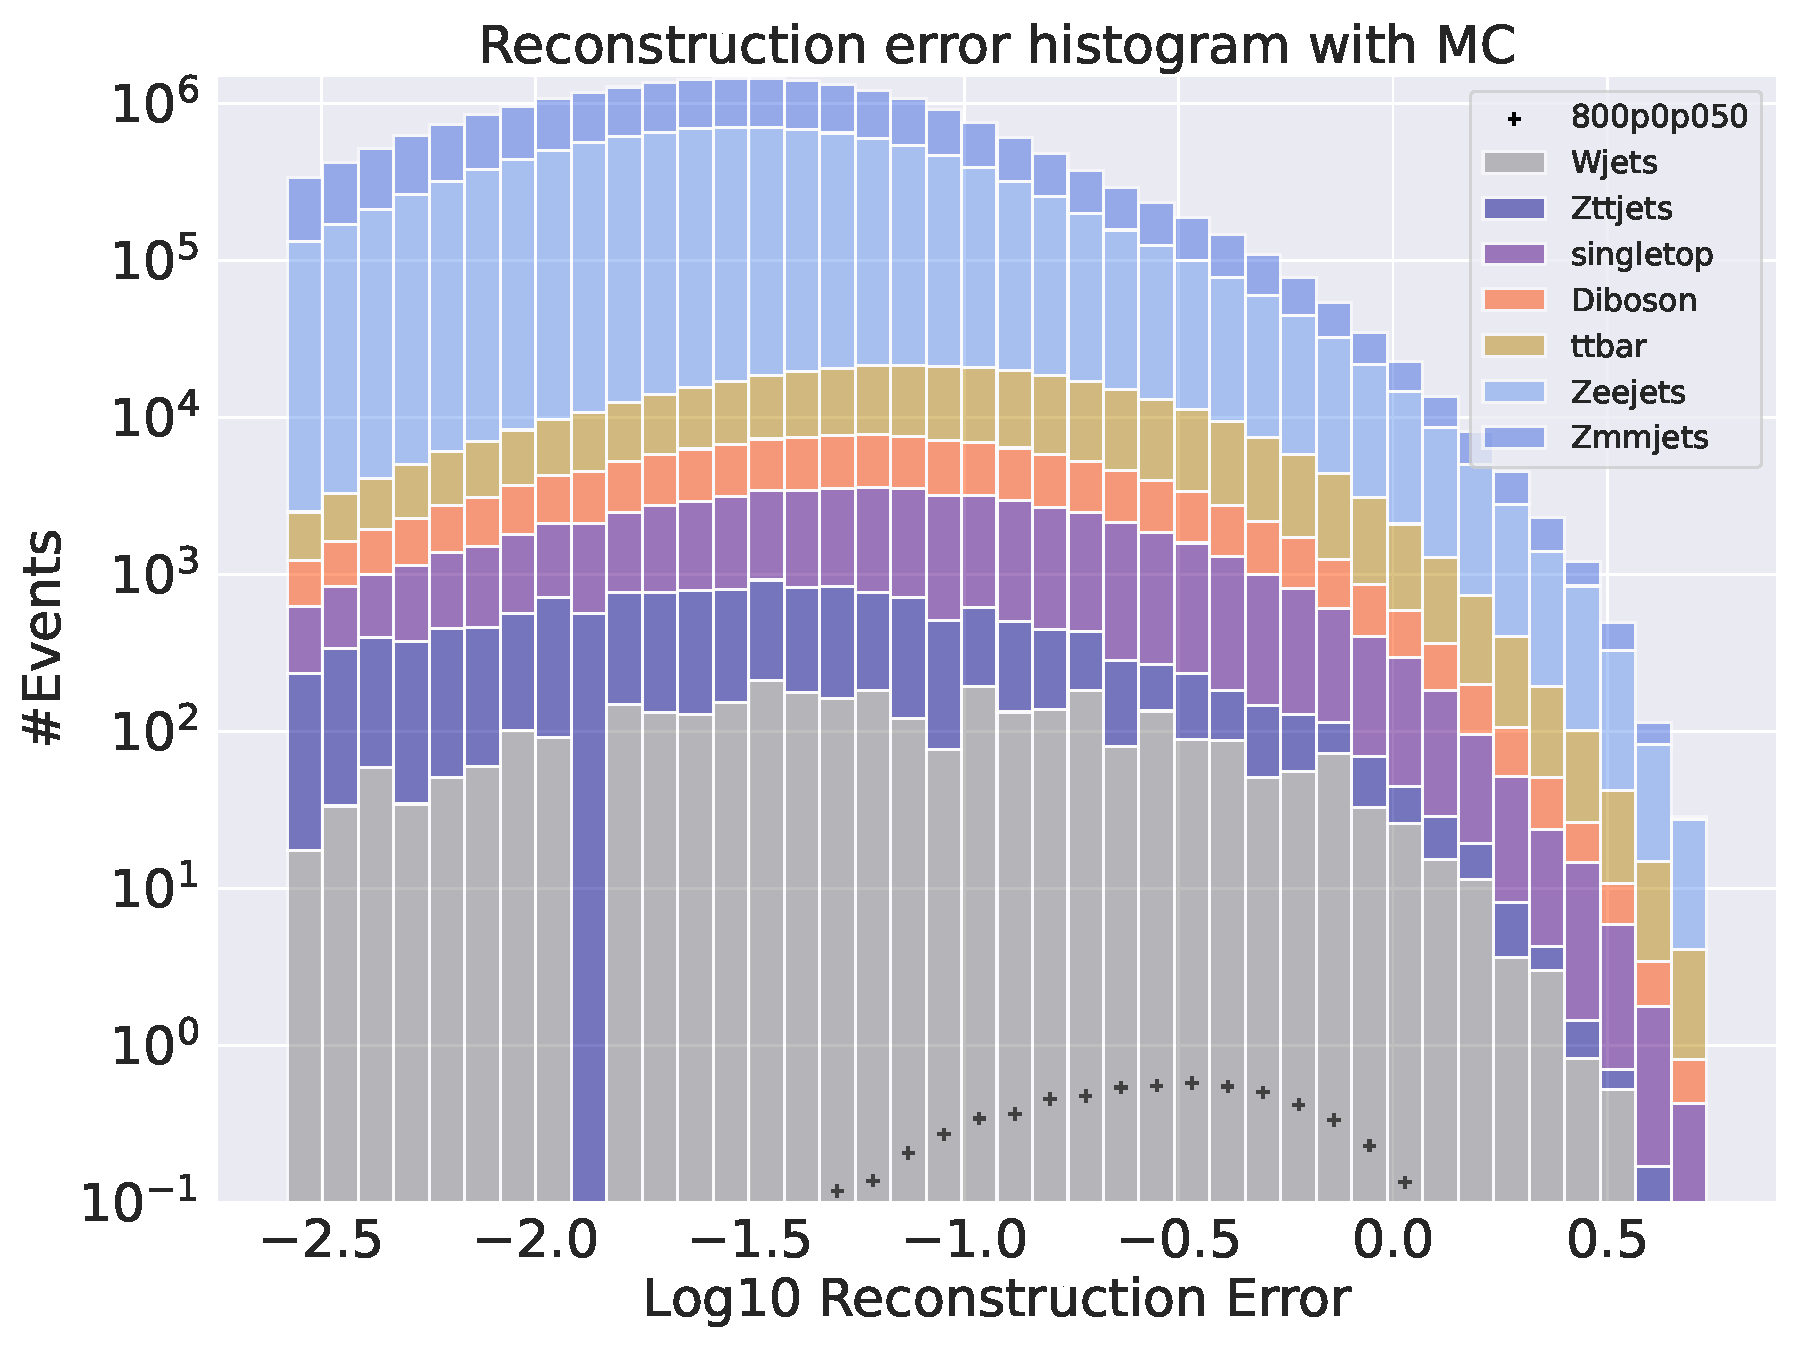
\includegraphics[width=\textwidth]{Figures/VAE_testing/big/2lep/b_data_recon_big_rm3_feats_sig_800p0p050_.pdf}
        \caption{ }
        \label{fig:VAE_2lep_big_800_2}
    \end{subfigure}
    \hfill
    \begin{subfigure}{.40\textwidth}
        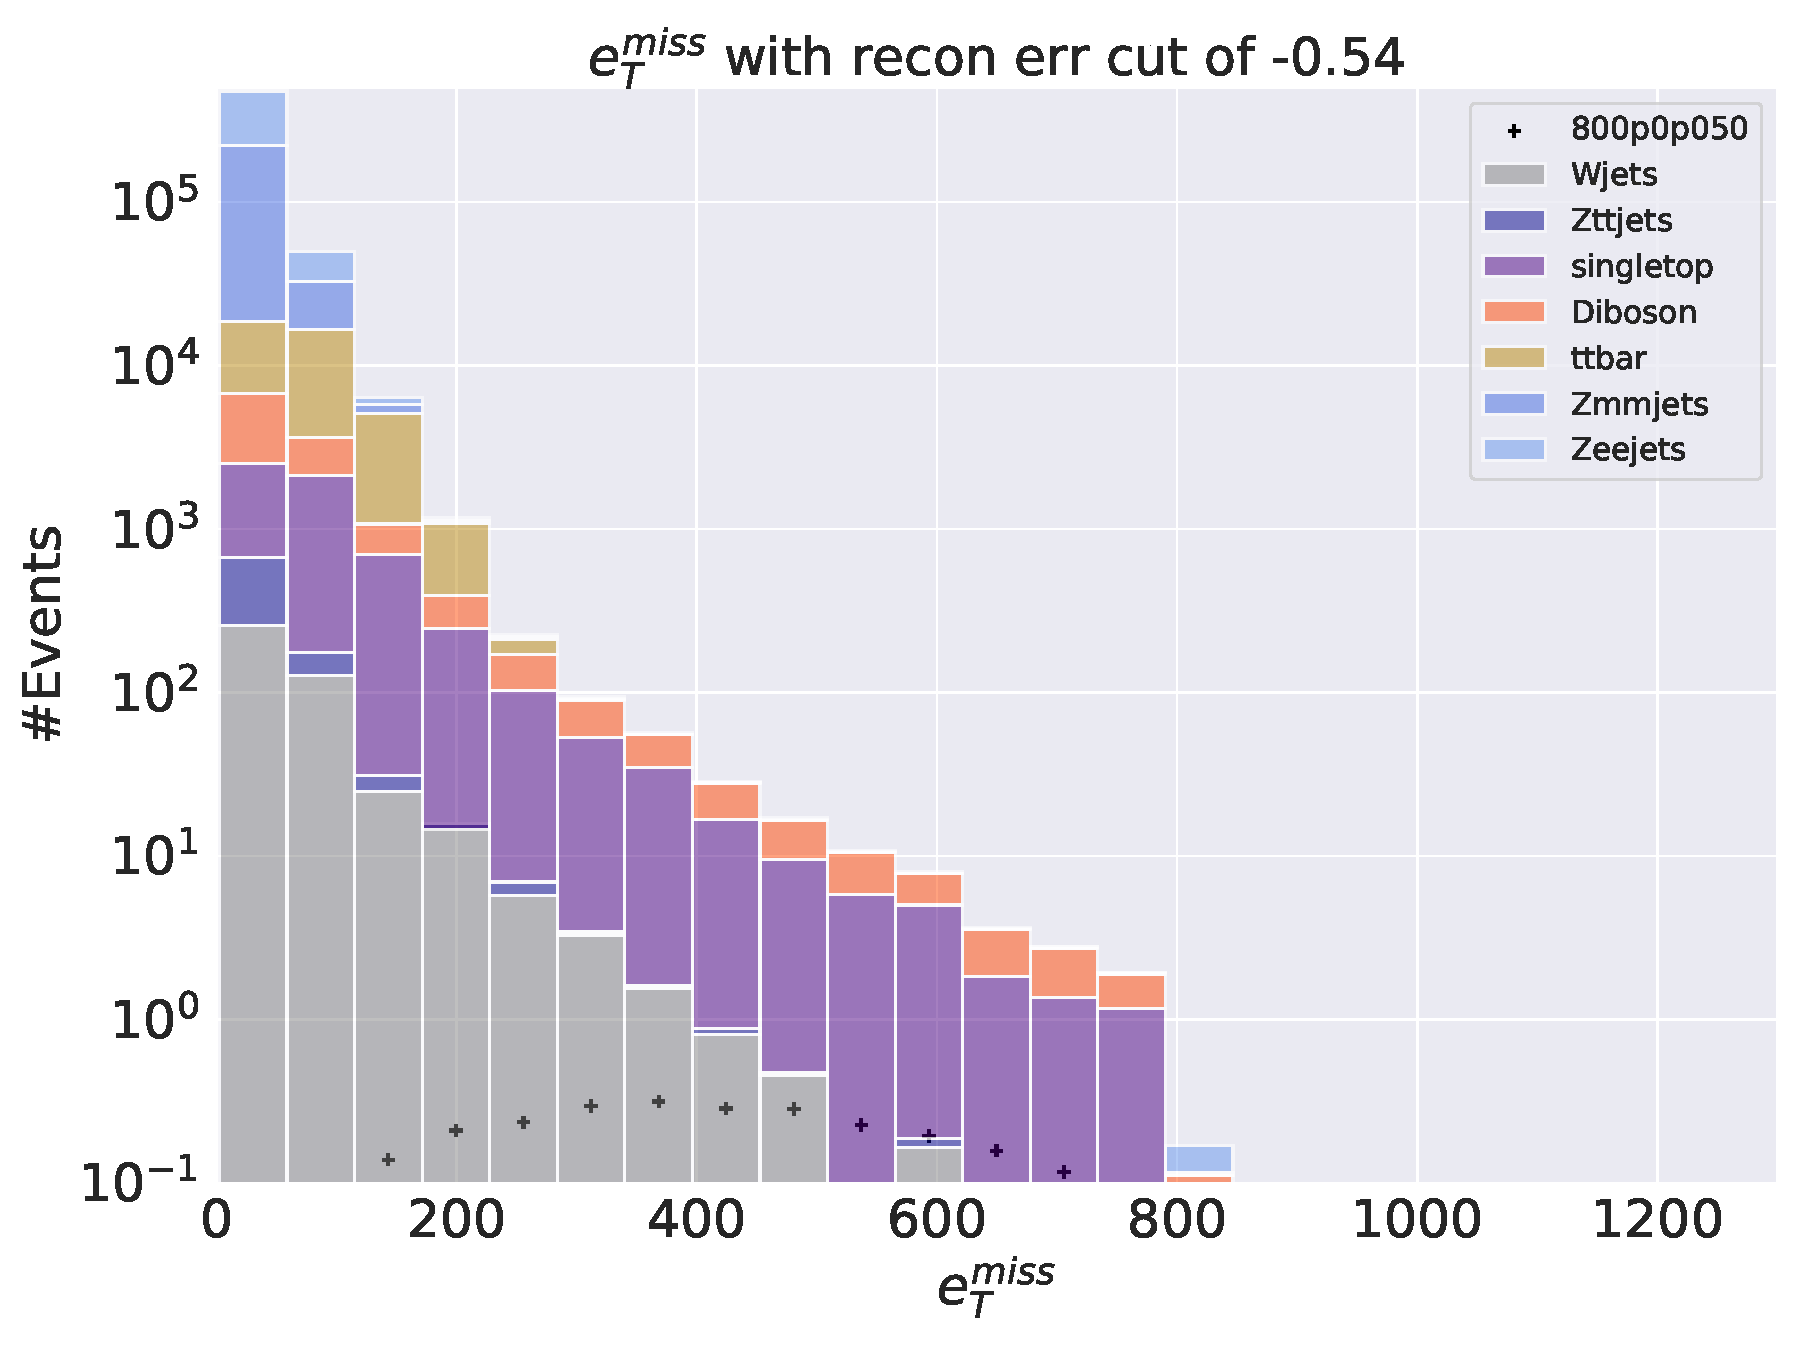
\includegraphics[width=\textwidth]{Figures/VAE_testing/big/2lep/b_data_recon_big_rm3_feats_sig_800p0p050_recon_errcut_-0.54.pdf}
        \caption{}
        \label{fig:VAE_2lep_big_etmiss_800_2}
    \end{subfigure}
    \hfill
      
    \begin{subfigure}{.40\textwidth}
        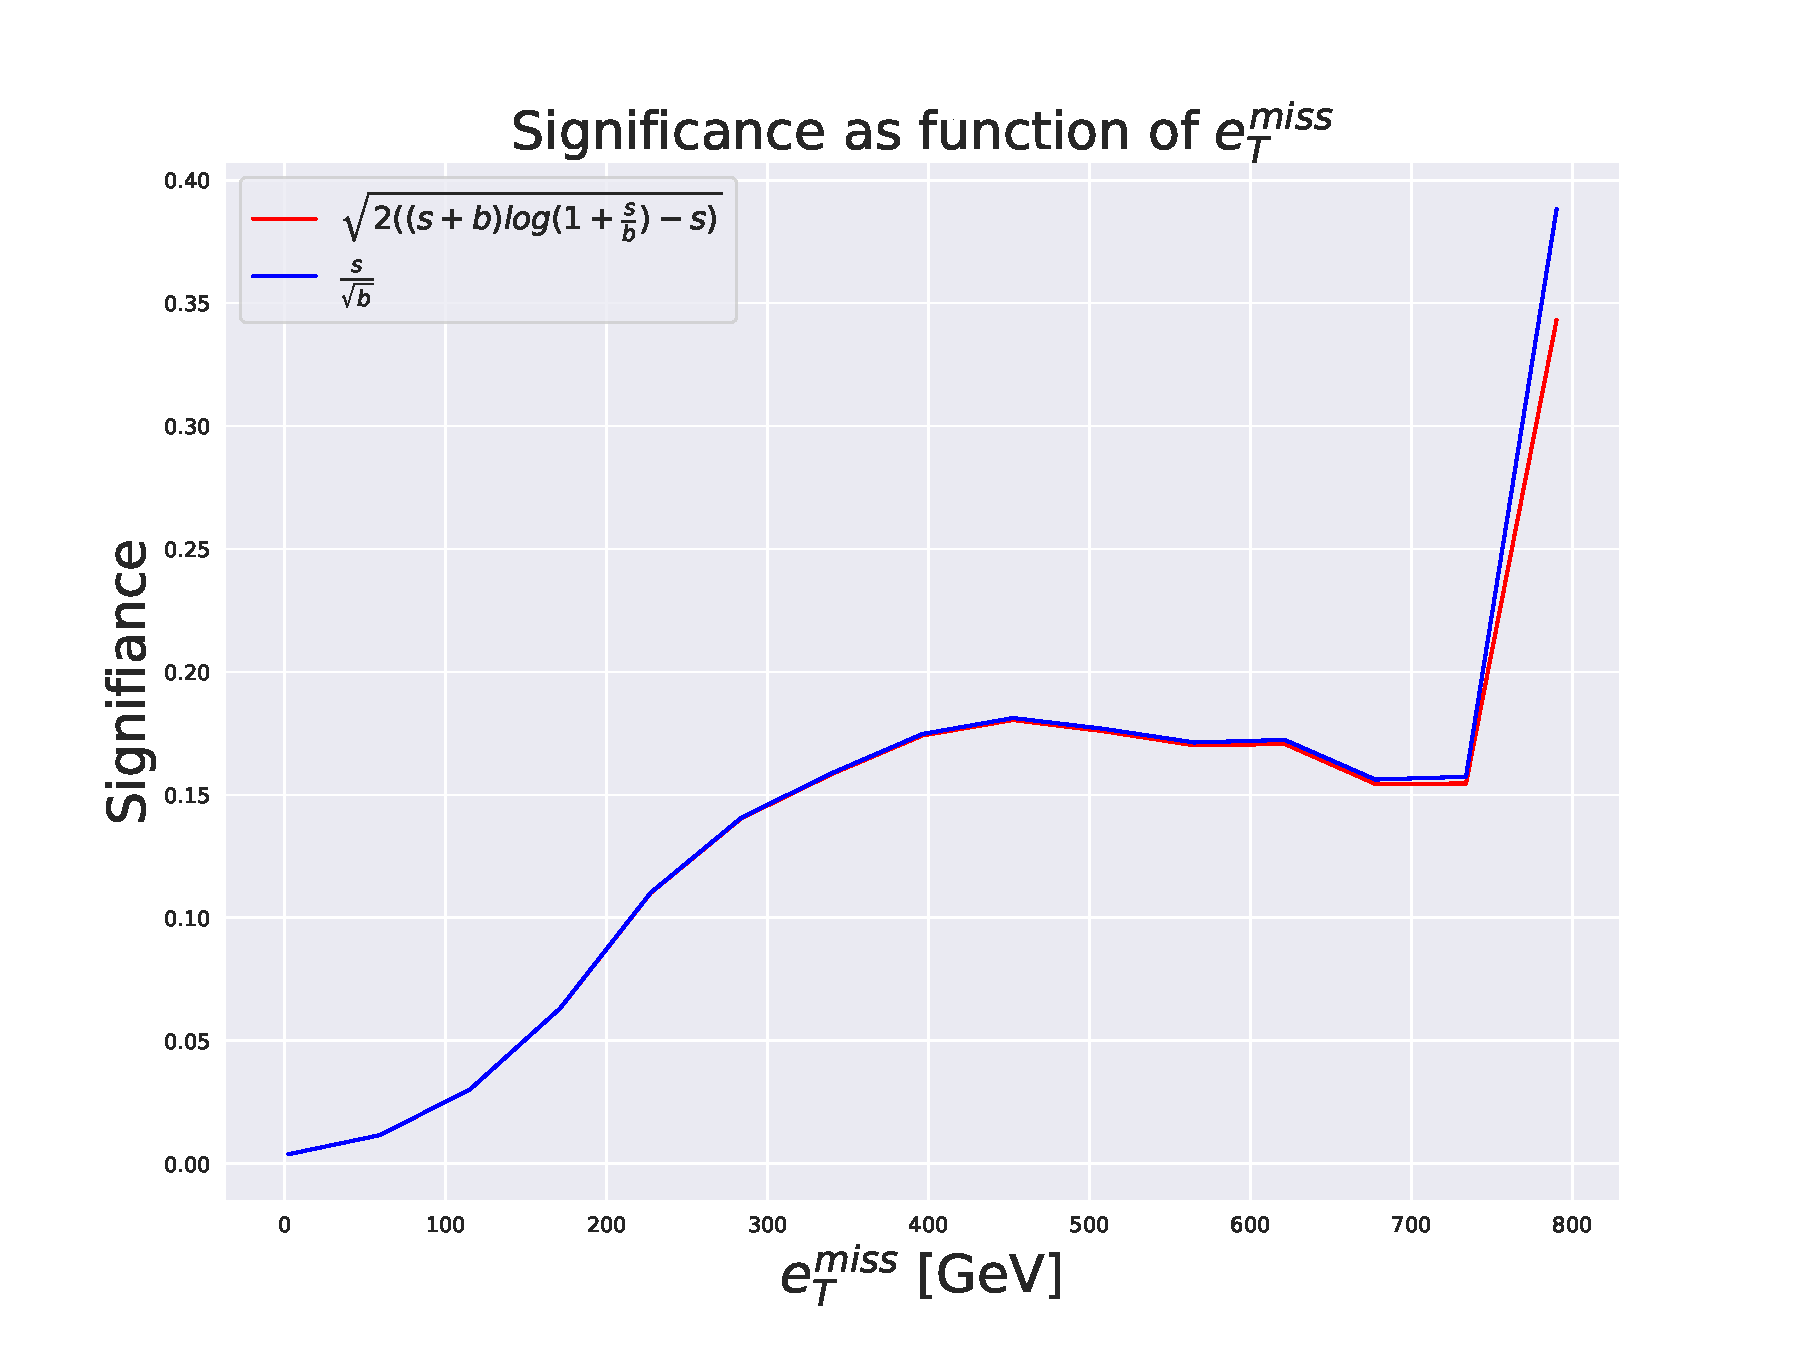
\includegraphics[width=\textwidth]{Figures/VAE_testing/big/2lep/significance_etmiss_800p0p050_-0.542414800898212.pdf}
        \caption{}
        \label{fig:VAE_2lep_big_signi_800_2}
    \end{subfigure}
    \hfill      
    \caption[2lep deep network | $800p50$ | VAE | 2]{Reconstruction error, $e_T^{miss}$ signal region, $m_{lll}$ signal region and significance as function of 
    $e_T^{miss}$ for the deep regular autoencoder. Here the SUSY $800p50$ model is used.}
    \label{fig:VAE_2lep_big_rec_sig_signi_800_2}
\end{figure}

\begin{figure}[H]
    \centering
    \begin{subfigure}{.40\textwidth}
        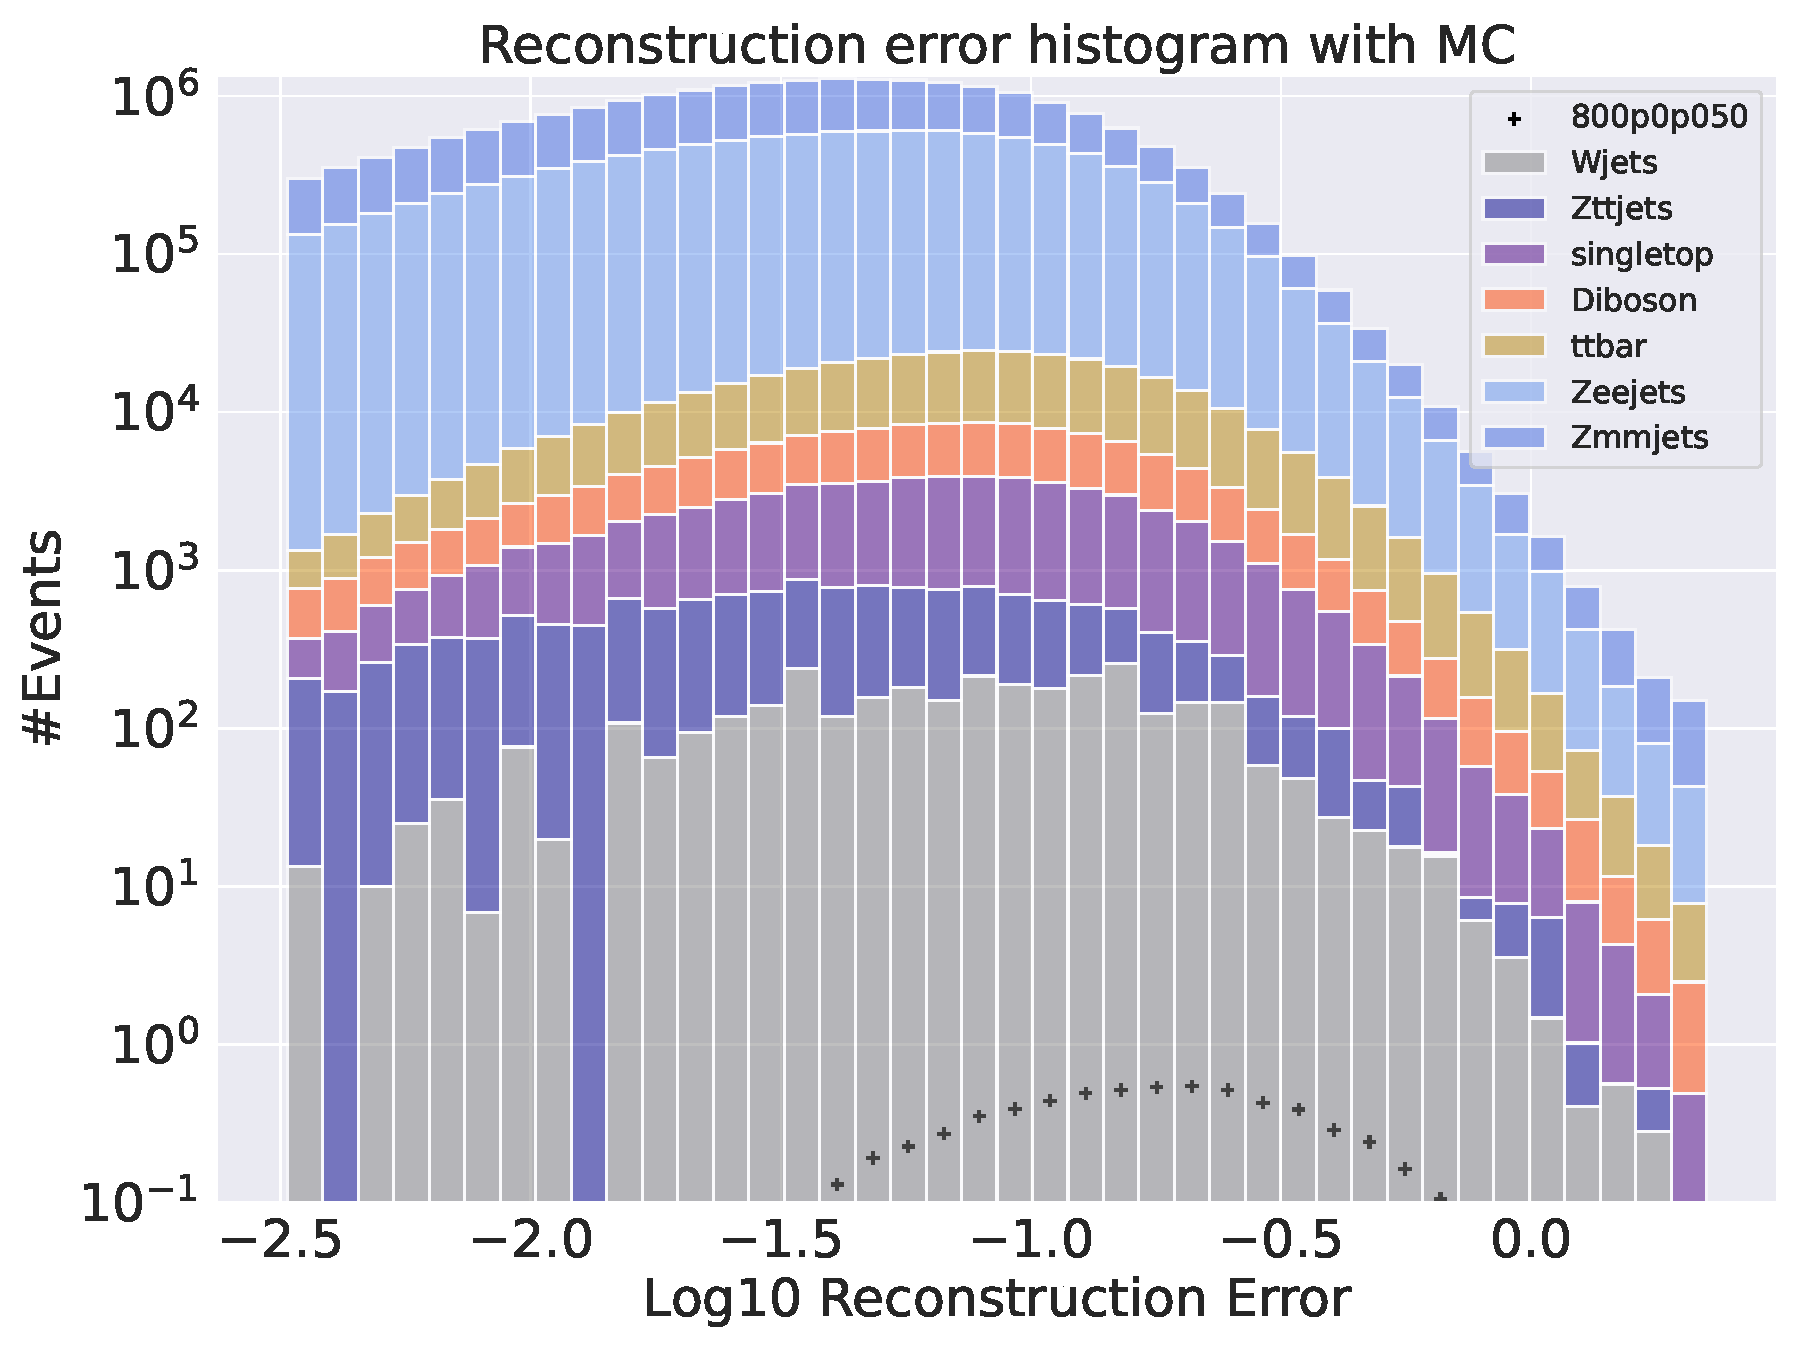
\includegraphics[width=\textwidth]{Figures/VAE_testing/small/2lep/b_data_recon_big_rm3_feats_sig_800p0p050_.pdf}
        \caption{ }
        \label{fig:VAE_2lep_small_800_2}
    \end{subfigure}
    \hfill
    \begin{subfigure}{.40\textwidth}
        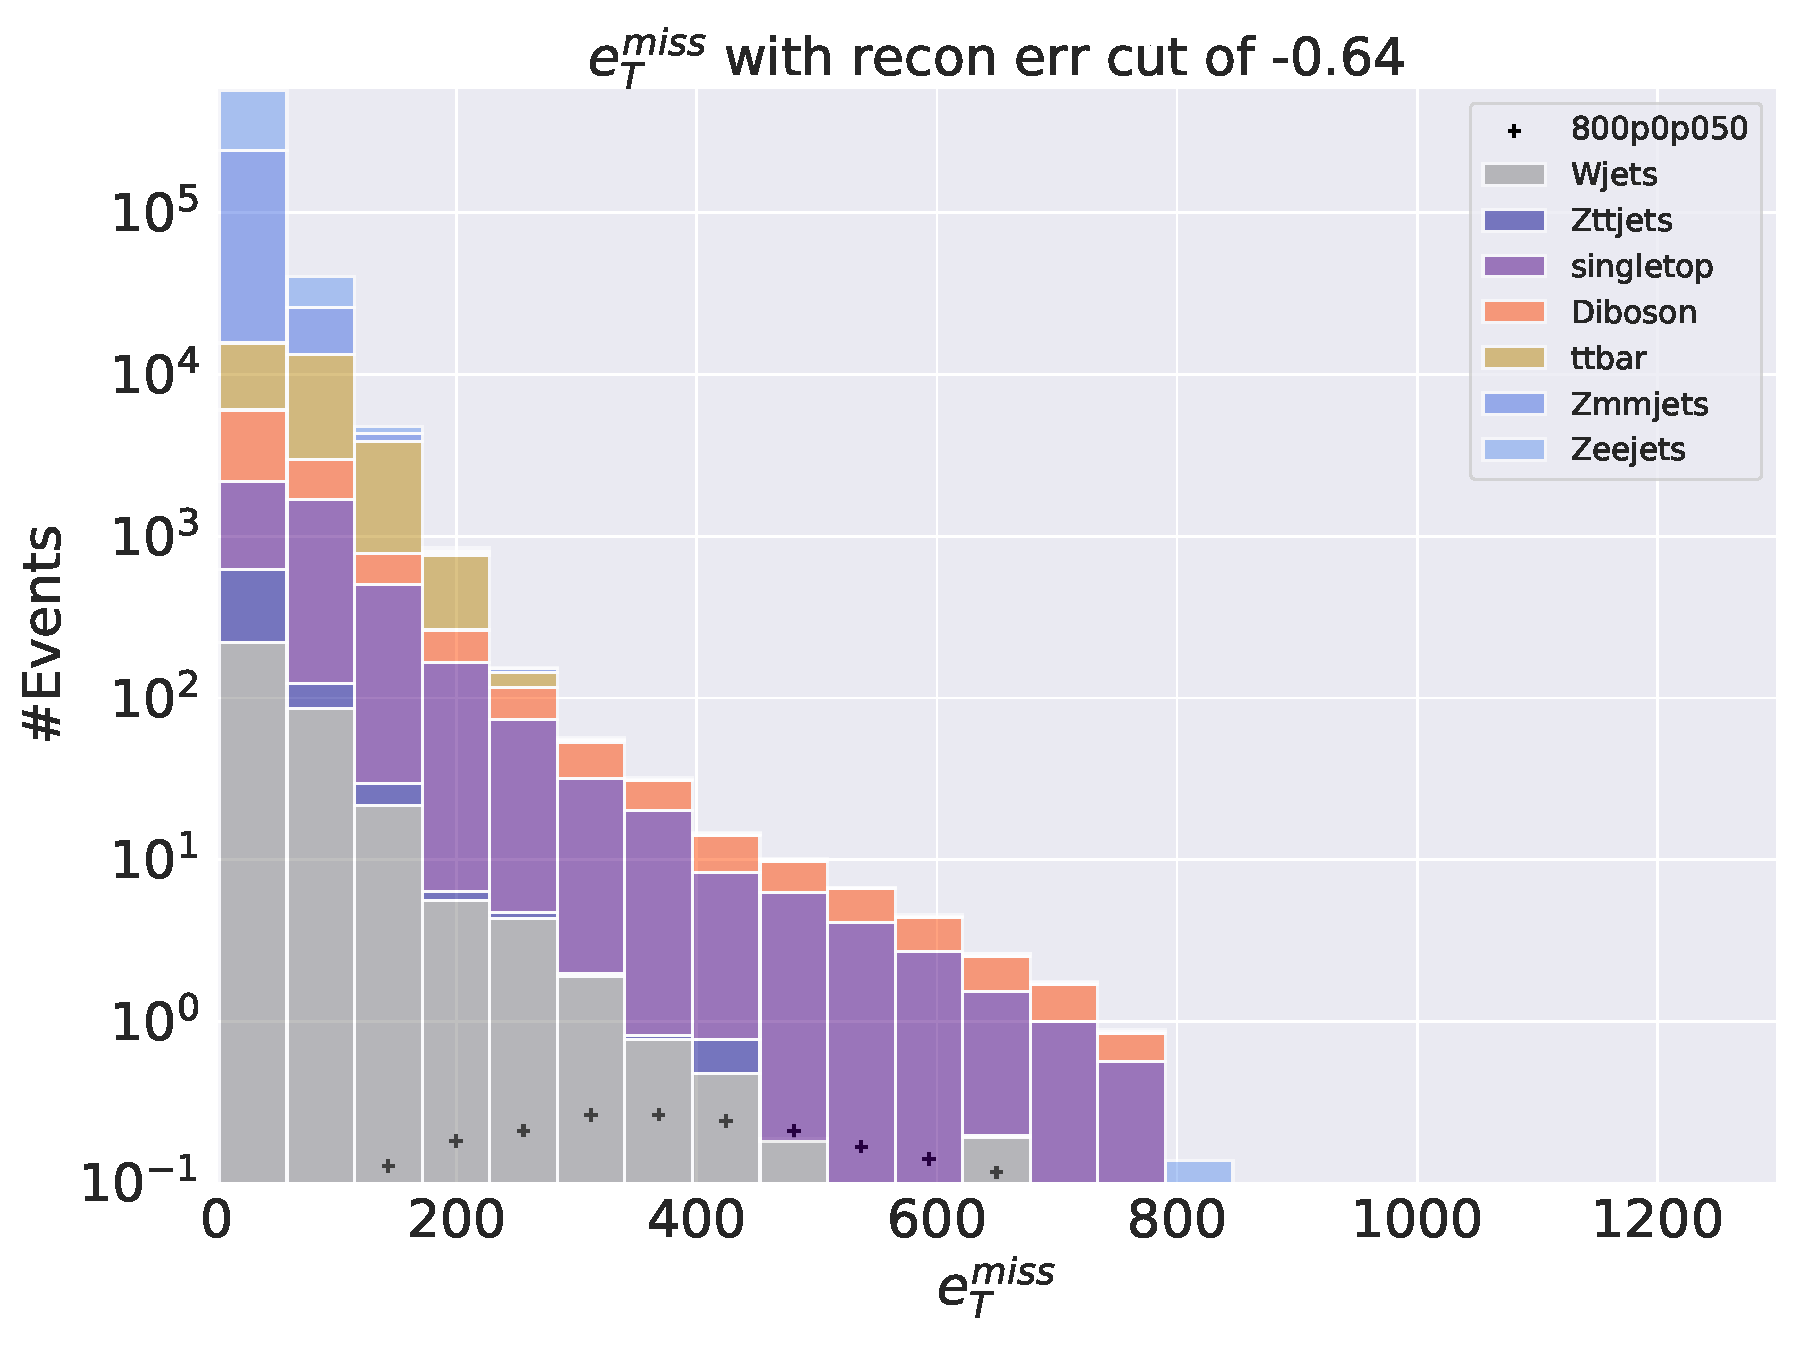
\includegraphics[width=\textwidth]{Figures/VAE_testing/small/2lep/b_data_recon_big_rm3_feats_sig_800p0p050_recon_errcut_-0.64.pdf}
        \caption{}
        \label{fig:VAE_2lep_small_etmiss_800_2}
    \end{subfigure}
    \hfill  
    \begin{subfigure}{.40\textwidth}
        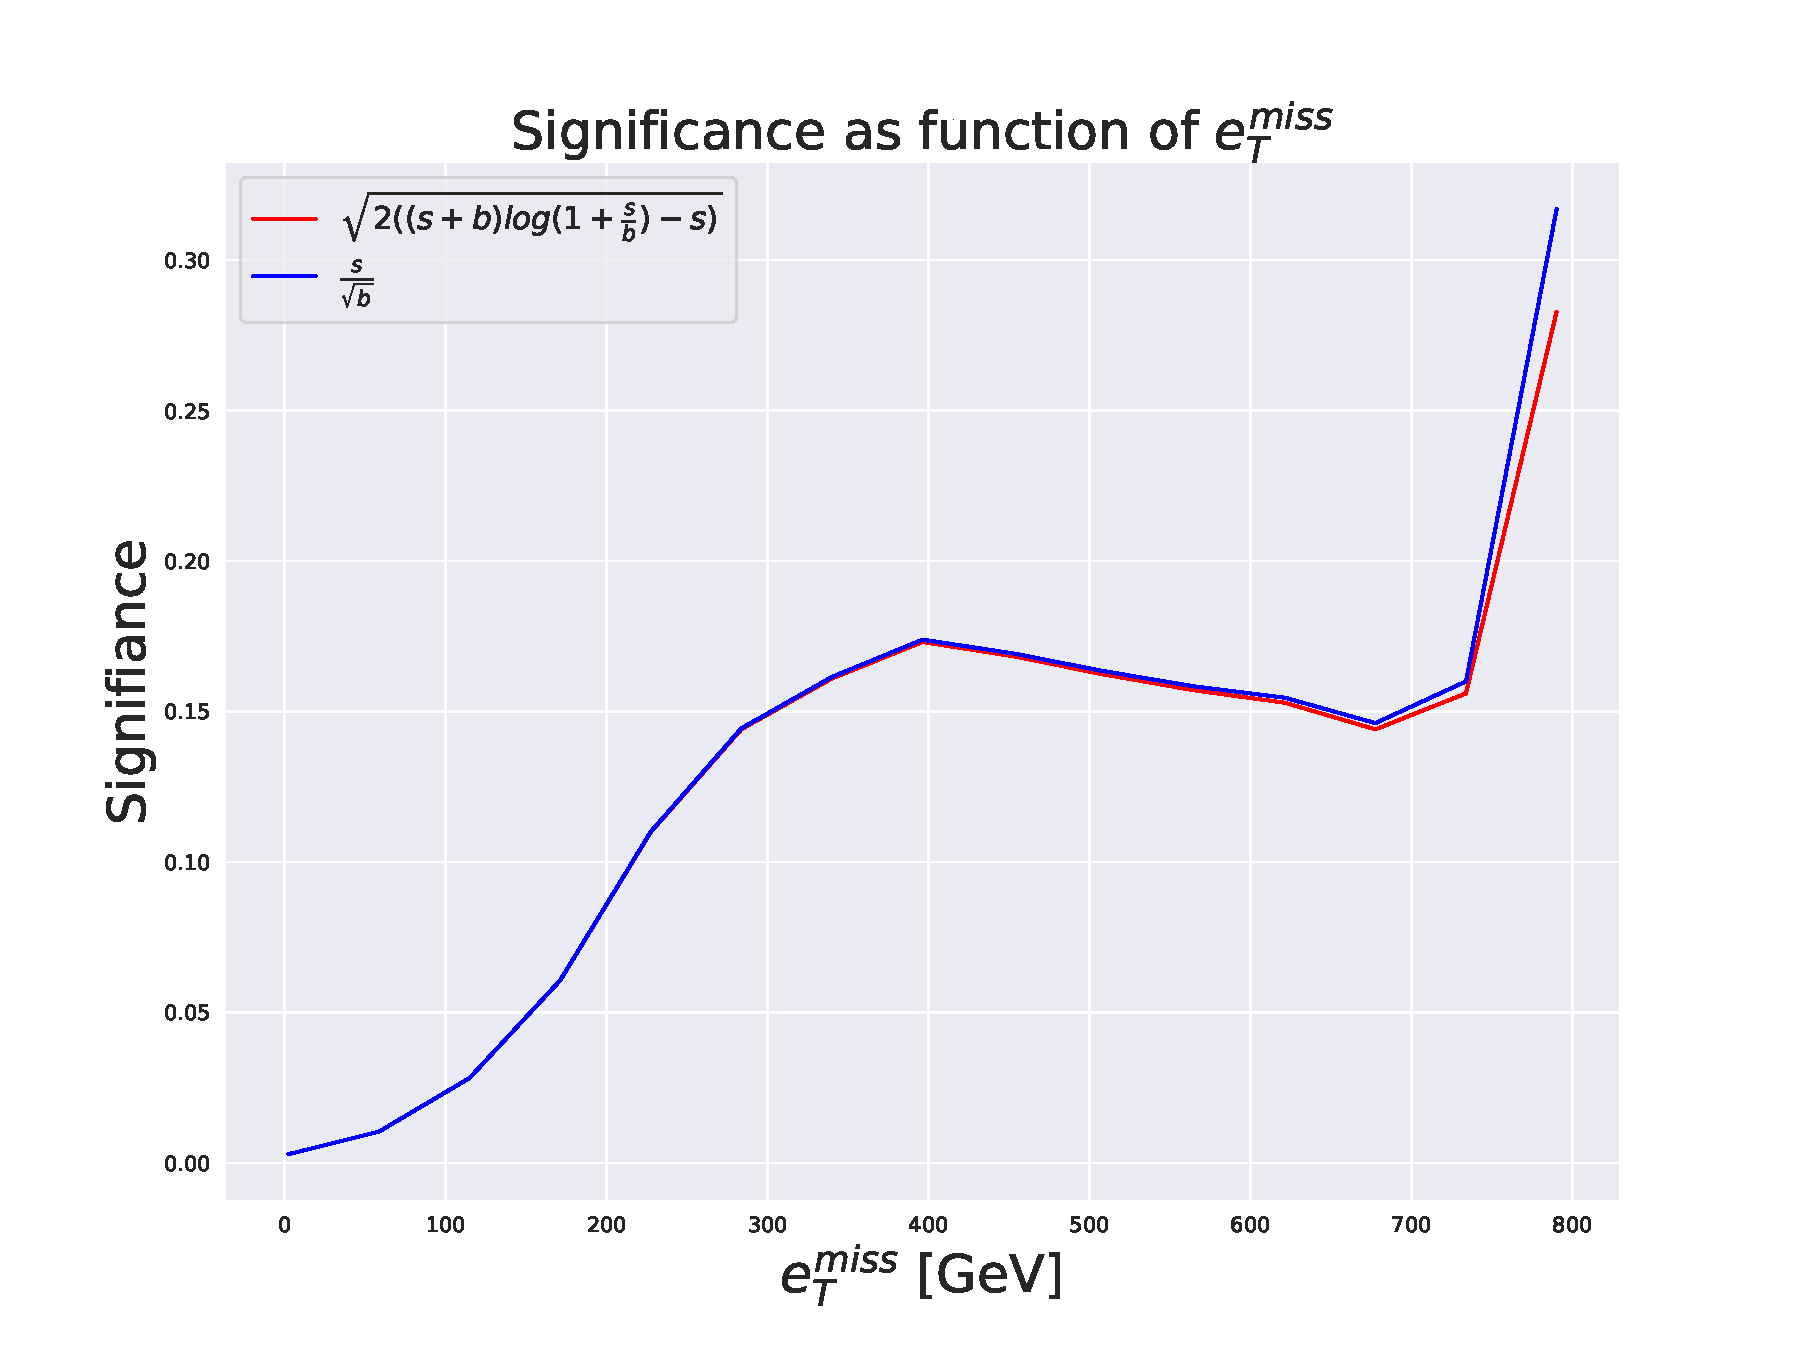
\includegraphics[width=\textwidth]{Figures/VAE_testing/small/2lep/significance_etmiss_800p0p050_-0.6406612200568815.pdf}
        \caption{}
        \label{fig:VAE_2lep_small_signi_800_2}
    \end{subfigure}
    \hfill      
    \caption[2lep shallow network | $800p50$ | VAE | 2]{Reconstruction error, $e_T^{miss}$ signal region, $m_{lll}$ signal region and significance as function of 
    $e_T^{miss}$ for the shallow regular autoencoder. Here the SUSY $800p50$ model is used.}
    \label{fig:VAE_2lep_small_rec_sig_signi_800_2}
\end{figure}




























\begin{figure}[H]
    \centering
    \begin{subfigure}{.40\textwidth}
        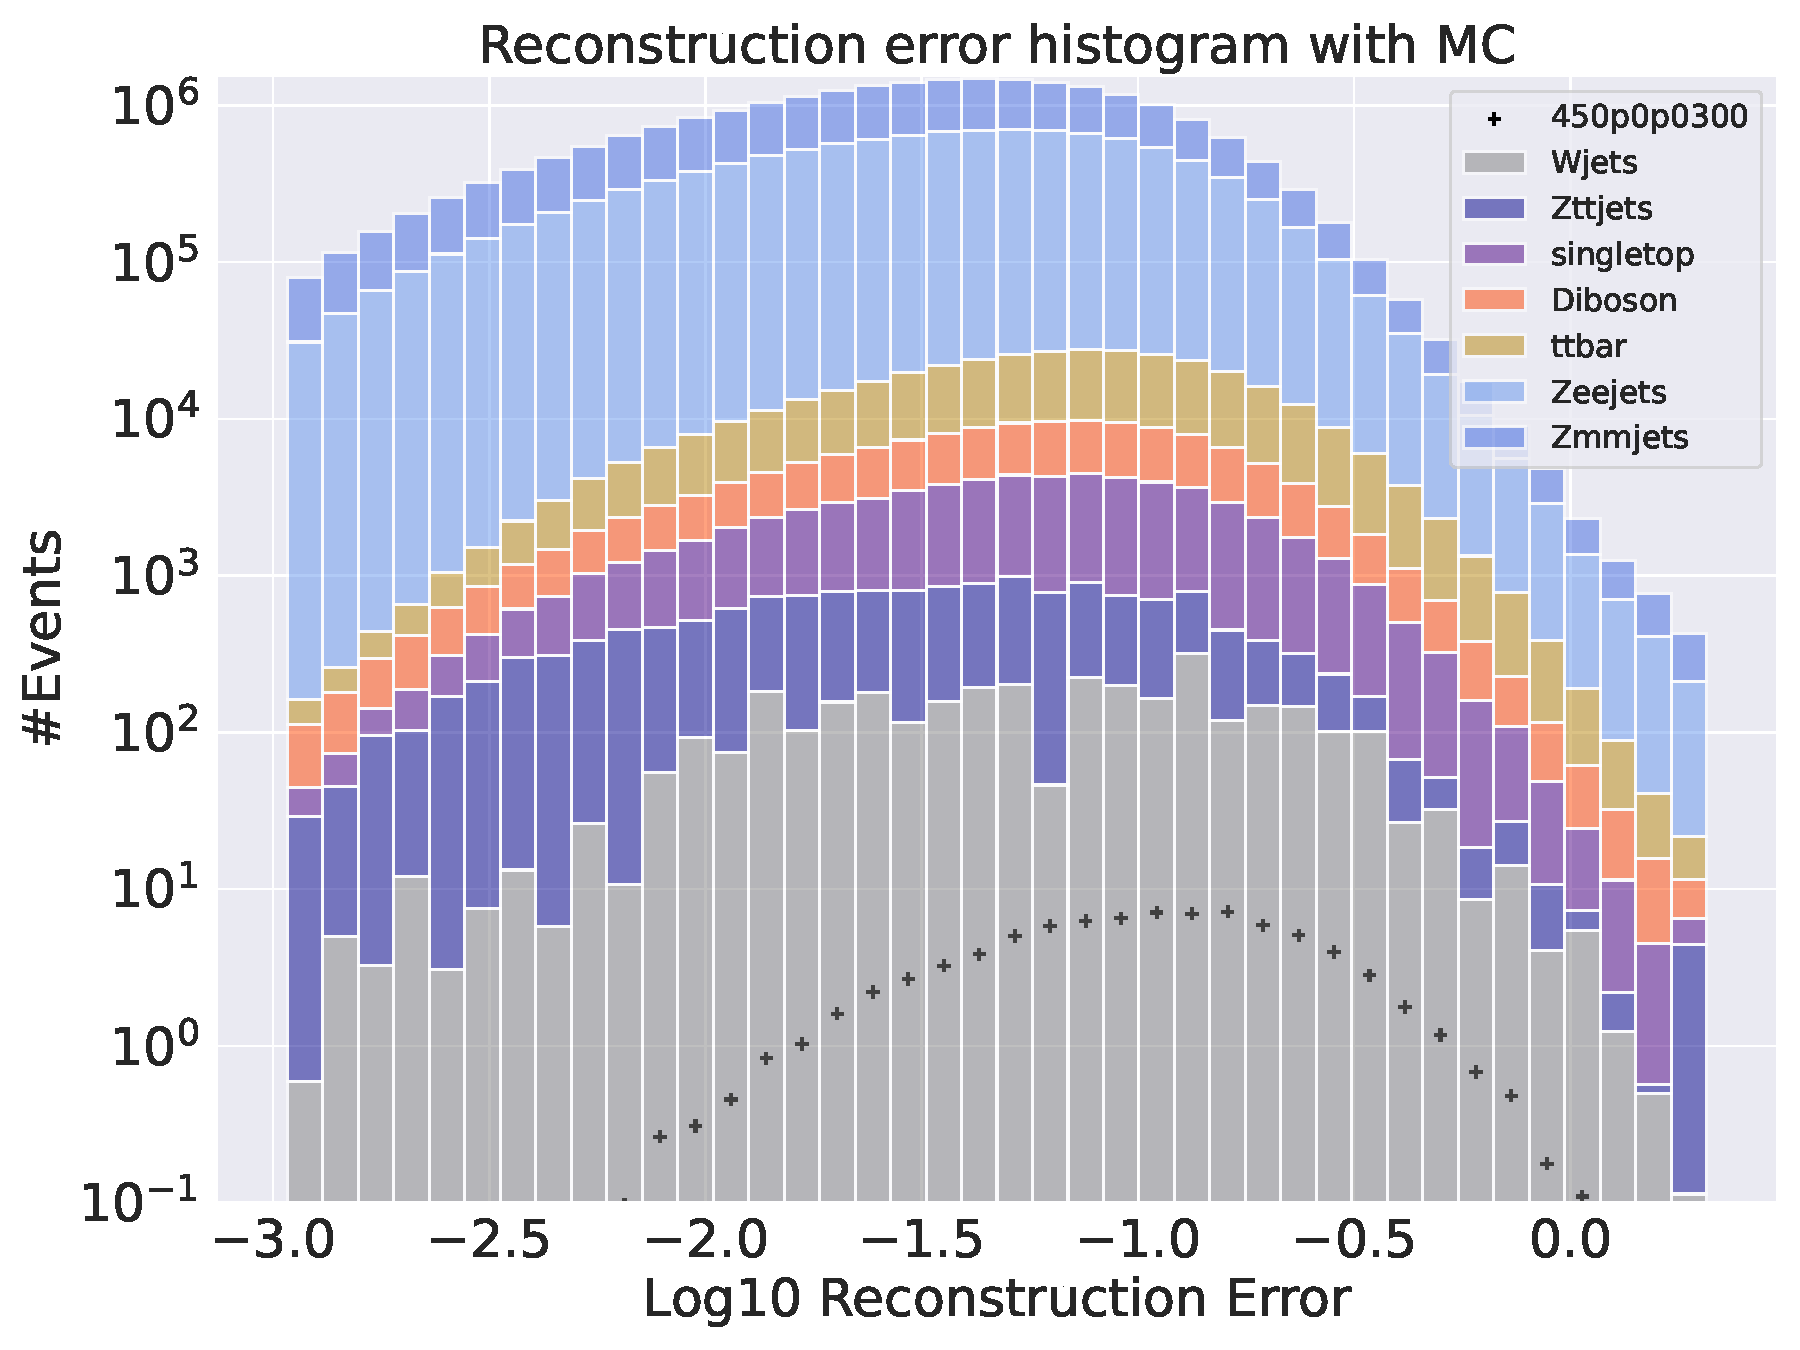
\includegraphics[width=\textwidth]{Figures/VAE_testing/small/2lep/b_data_recon_big_rm3_feats_sig_450p0p0300_.pdf}
        \caption{ }
        \label{fig:VAE_2lep_big_450_3}
    \end{subfigure}
    \hfill
    \begin{subfigure}{.40\textwidth}
        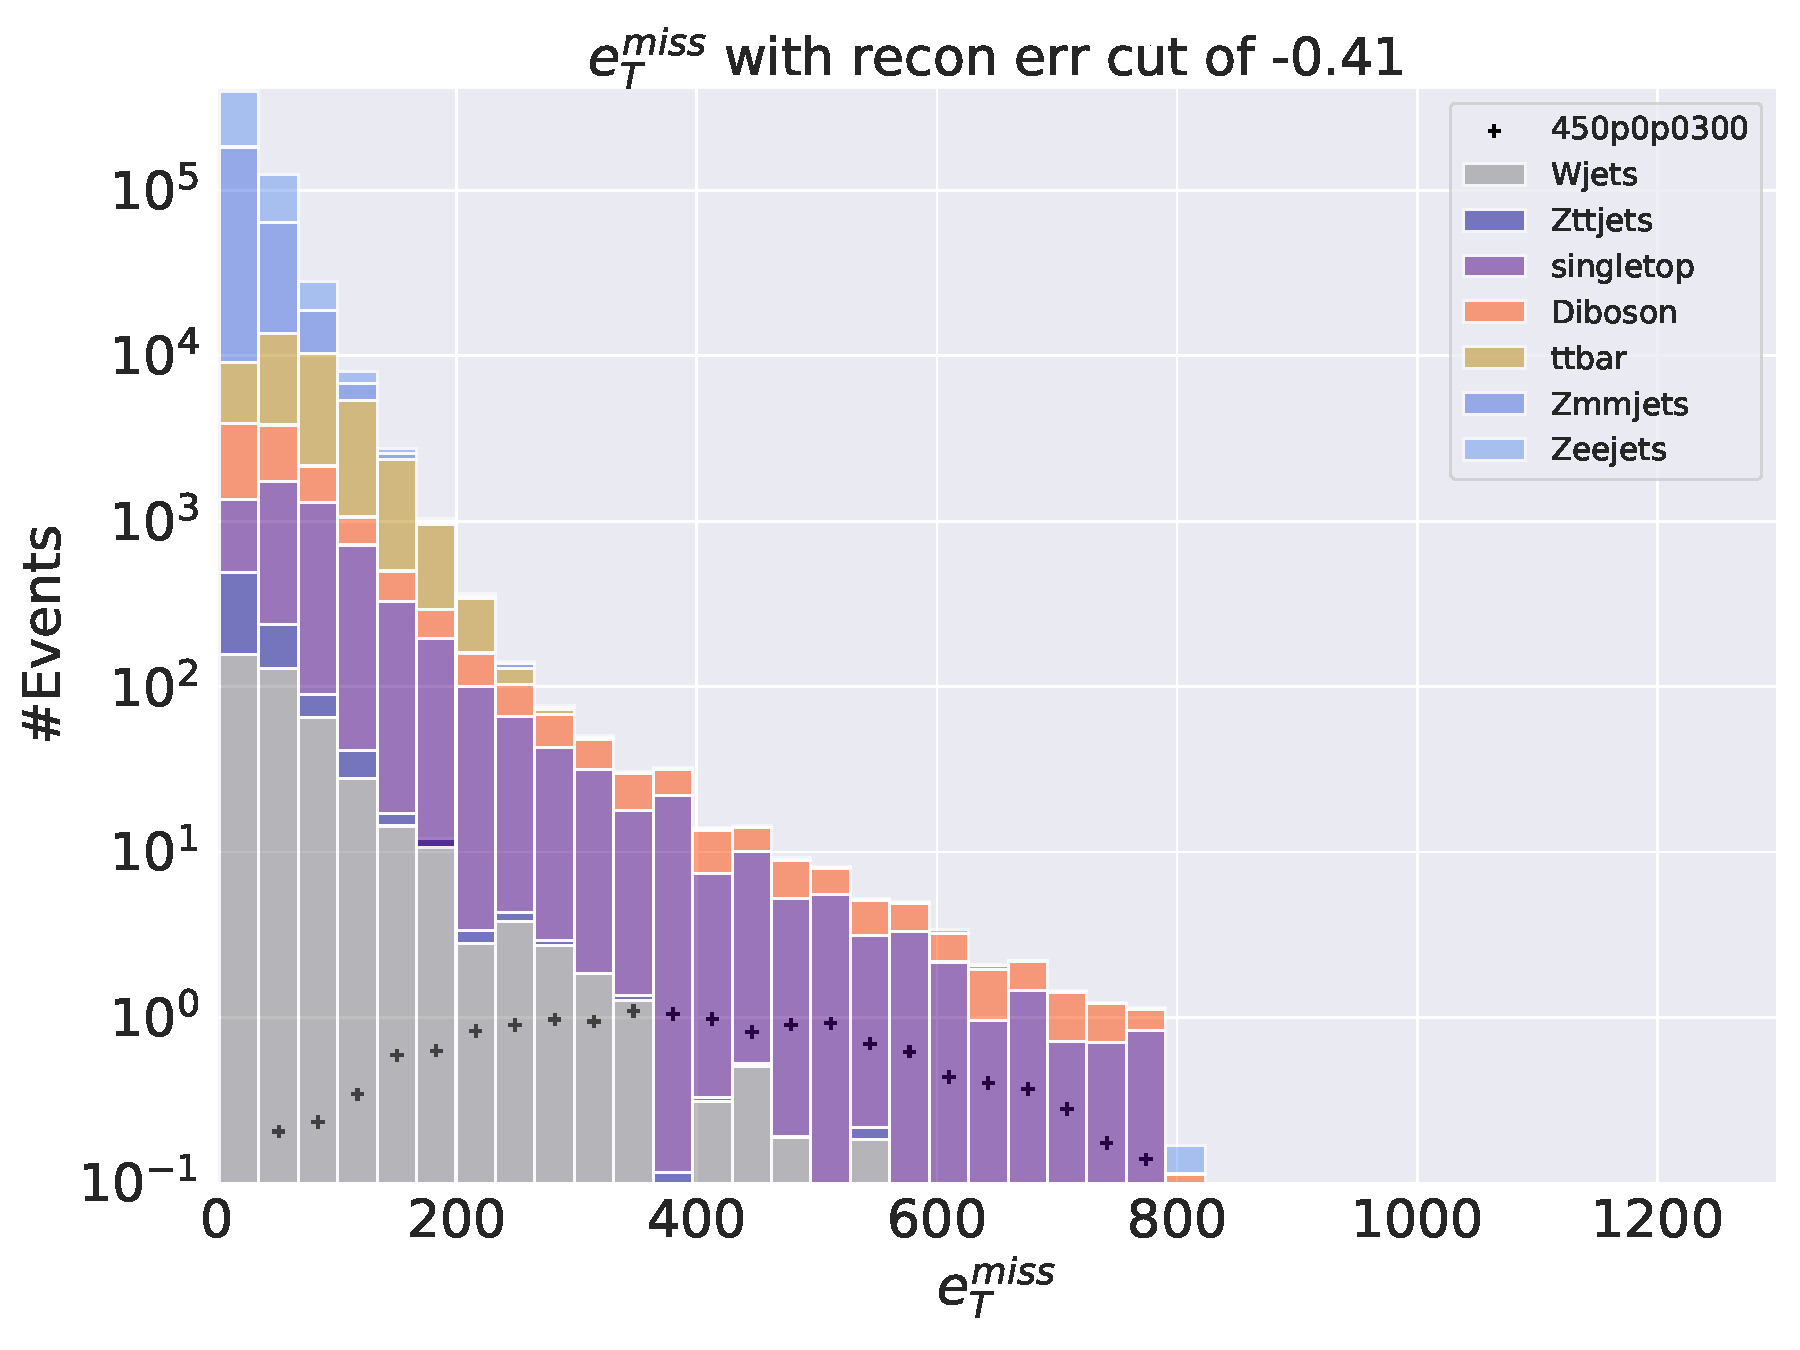
\includegraphics[width=\textwidth]{Figures/VAE_testing/big/2lep/b_data_recon_big_rm3_feats_sig_450p0p0300_recon_errcut_-0.41.pdf}
        \caption{}
        \label{fig:VAE_2lep_big_etmiss_450_3}
    \end{subfigure}
    \hfill 
    \begin{subfigure}{.40\textwidth}
        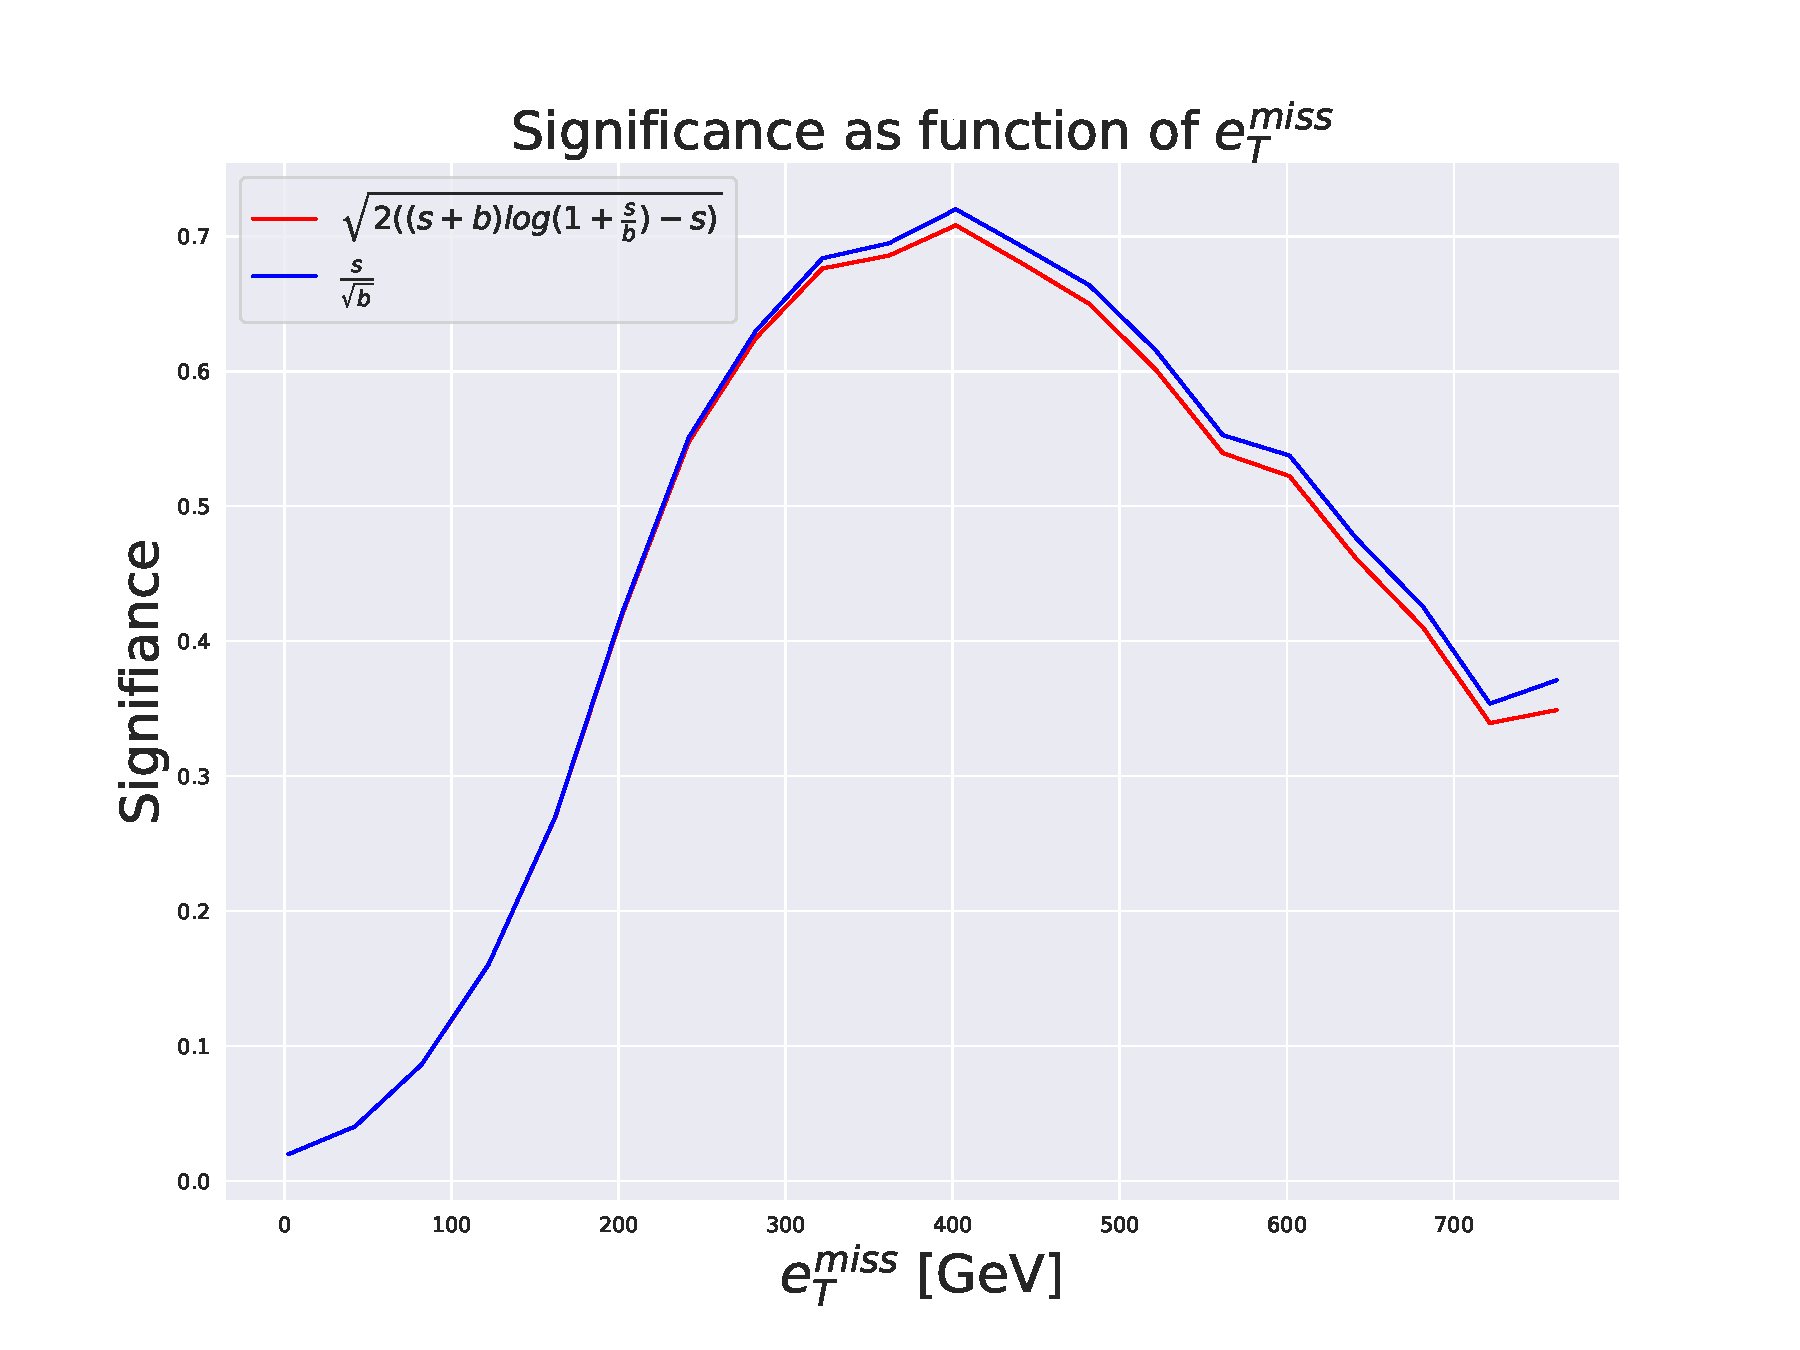
\includegraphics[width=\textwidth]{Figures/VAE_testing/big/2lep/significance_etmiss_450p0p0300_-0.40609370505539655.pdf}
        \caption{}
        \label{fig:VAE_2lep_big_signi_450_3}
    \end{subfigure}
    \hfill      
    \caption[2lep deep network | $450p300$ | VAE | 3]{Reconstruction error, $e_T^{miss}$ signal region, $m_{lll}$ signal region and significance as function of 
    $e_T^{miss}$ for the deep regular autoencoder. Here the SUSY $450p300$ model is used.}
    \label{fig:VAE_2lep_big_rec_sig_signi_450_3}
\end{figure}

\begin{figure}[H]
    \centering
    \begin{subfigure}{.40\textwidth}
        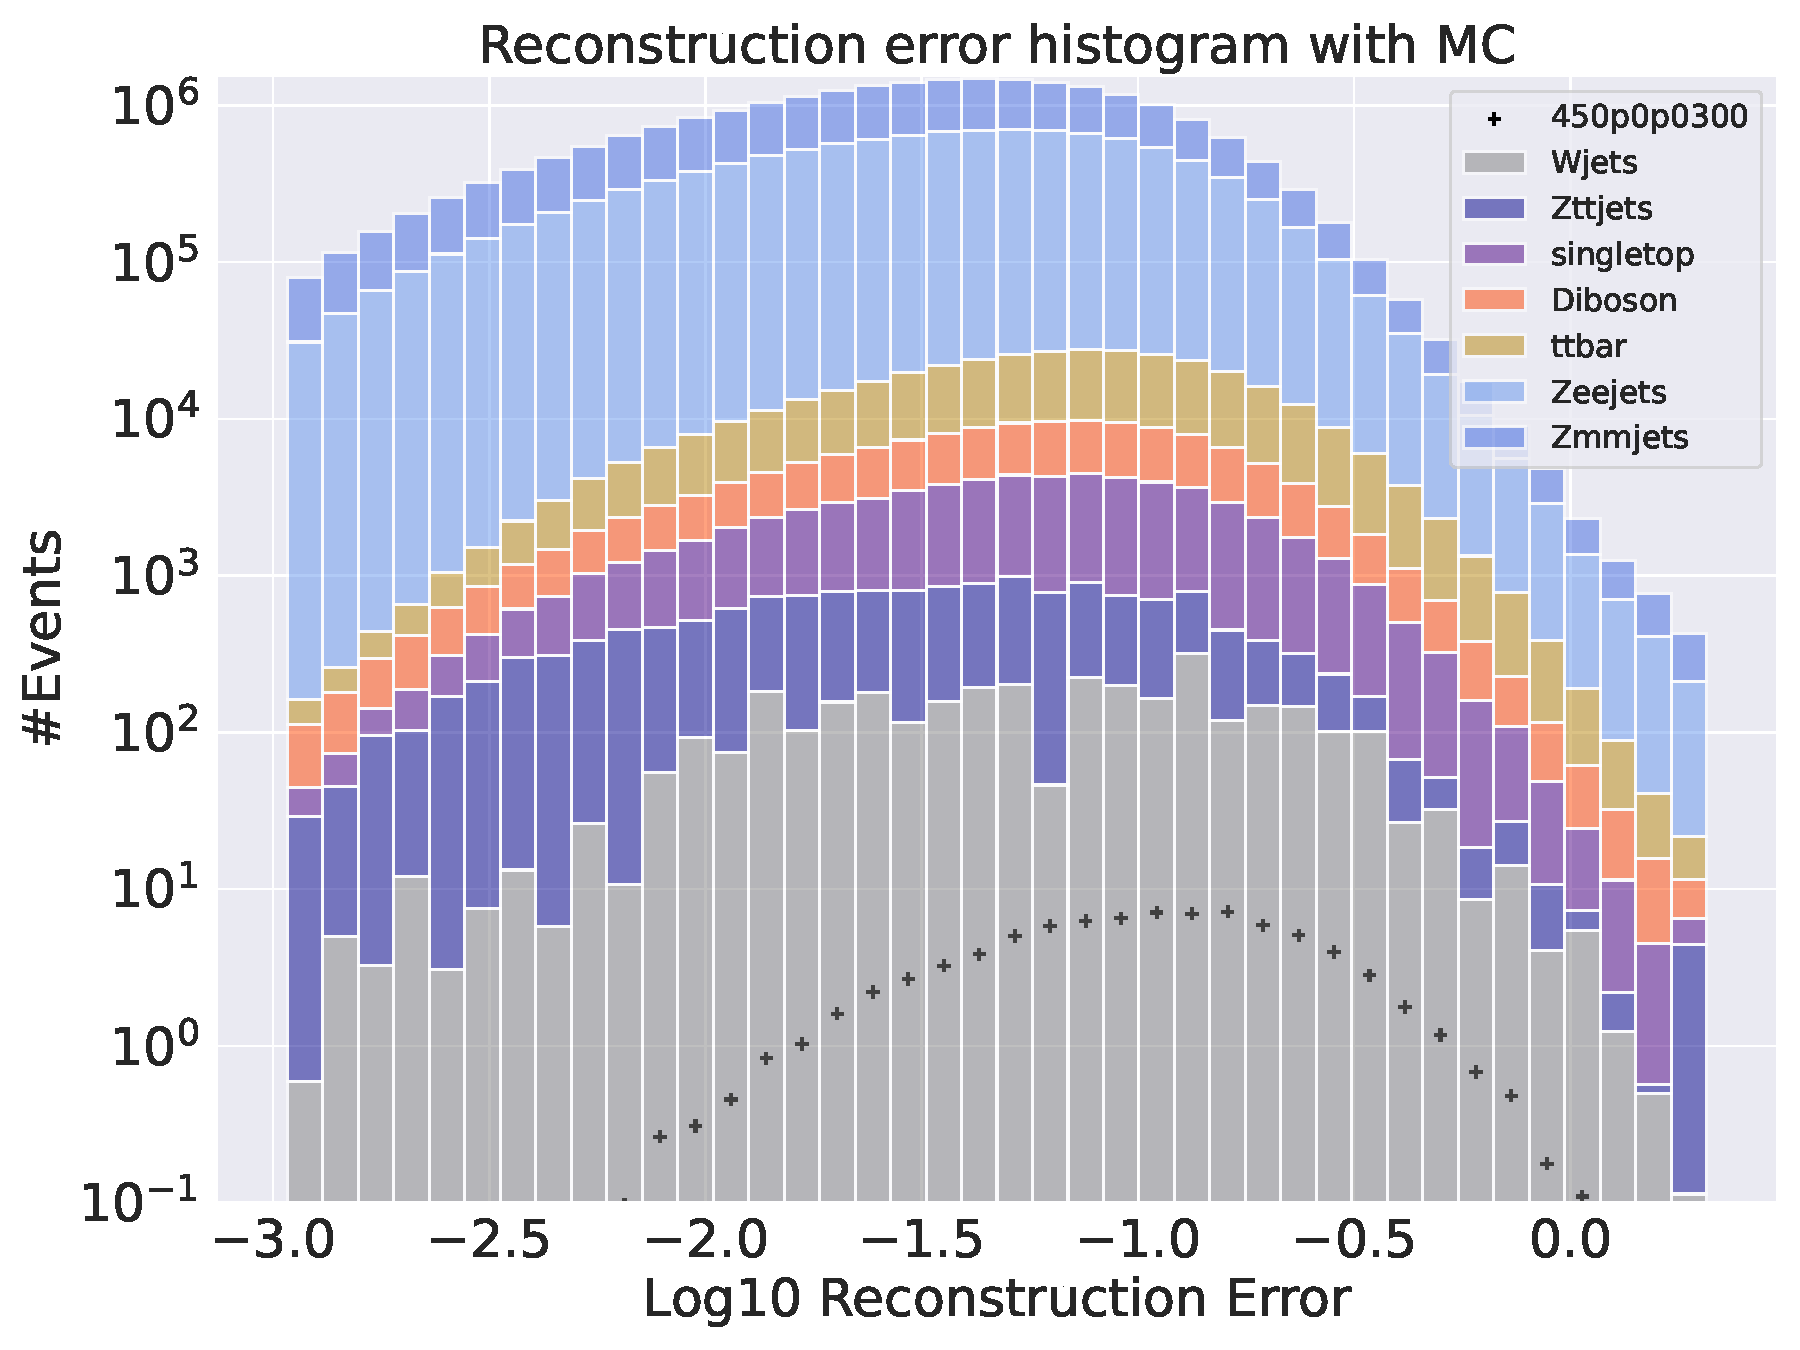
\includegraphics[width=\textwidth]{Figures/VAE_testing/small/2lep/b_data_recon_big_rm3_feats_sig_450p0p0300_.pdf}
        \caption{ }
        \label{fig:VAE_2lep_small_450_3}
    \end{subfigure}
    \hfill
    \begin{subfigure}{.40\textwidth}
        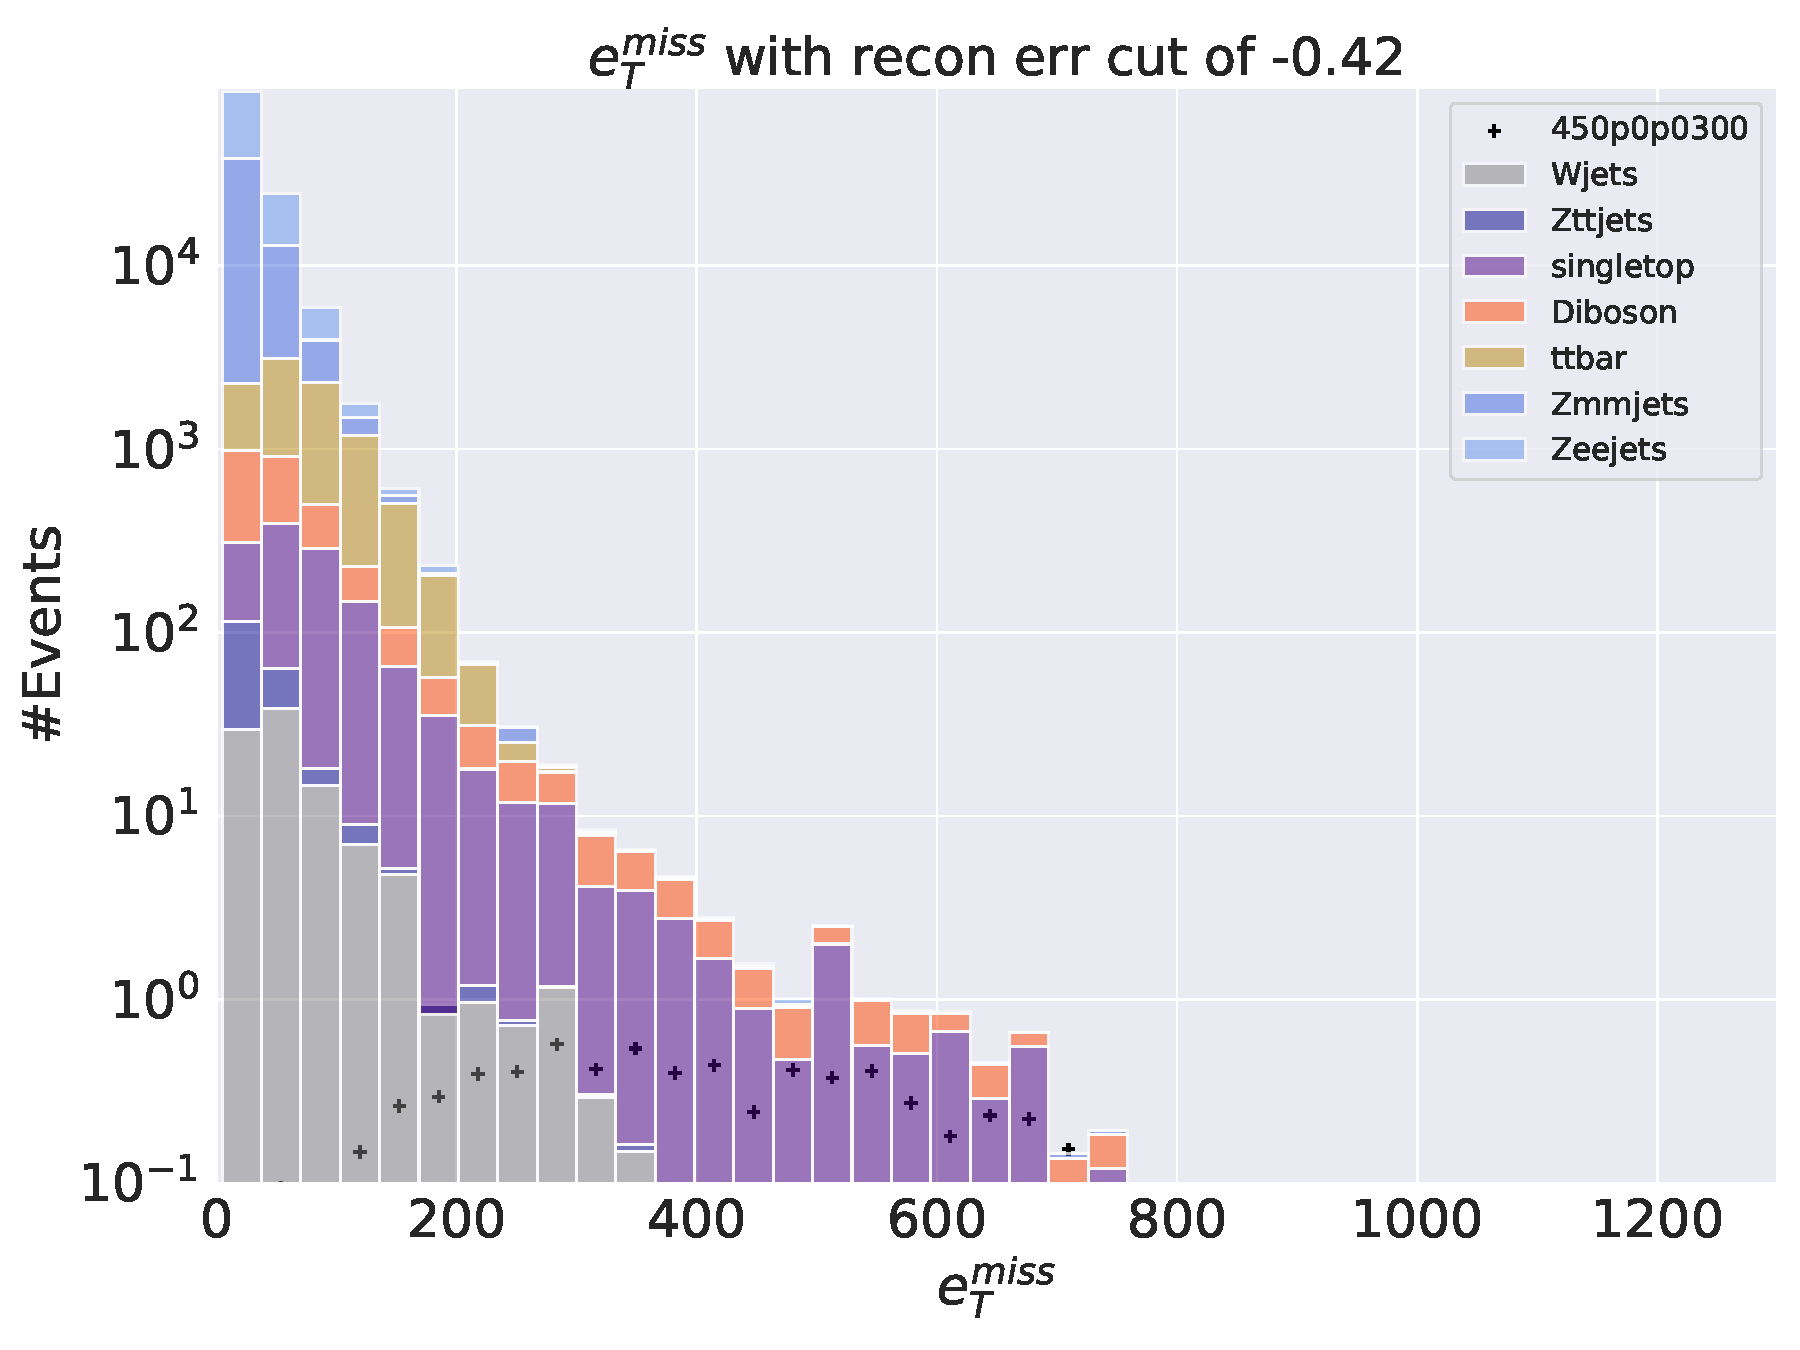
\includegraphics[width=\textwidth]{Figures/VAE_testing/small/2lep/b_data_recon_big_rm3_feats_sig_450p0p0300_recon_errcut_-0.42.pdf}
        \caption{}
        \label{fig:VAE_2lep_small_etmiss_450_3}
    \end{subfigure}
    \hfill  
    \begin{subfigure}{.40\textwidth}
        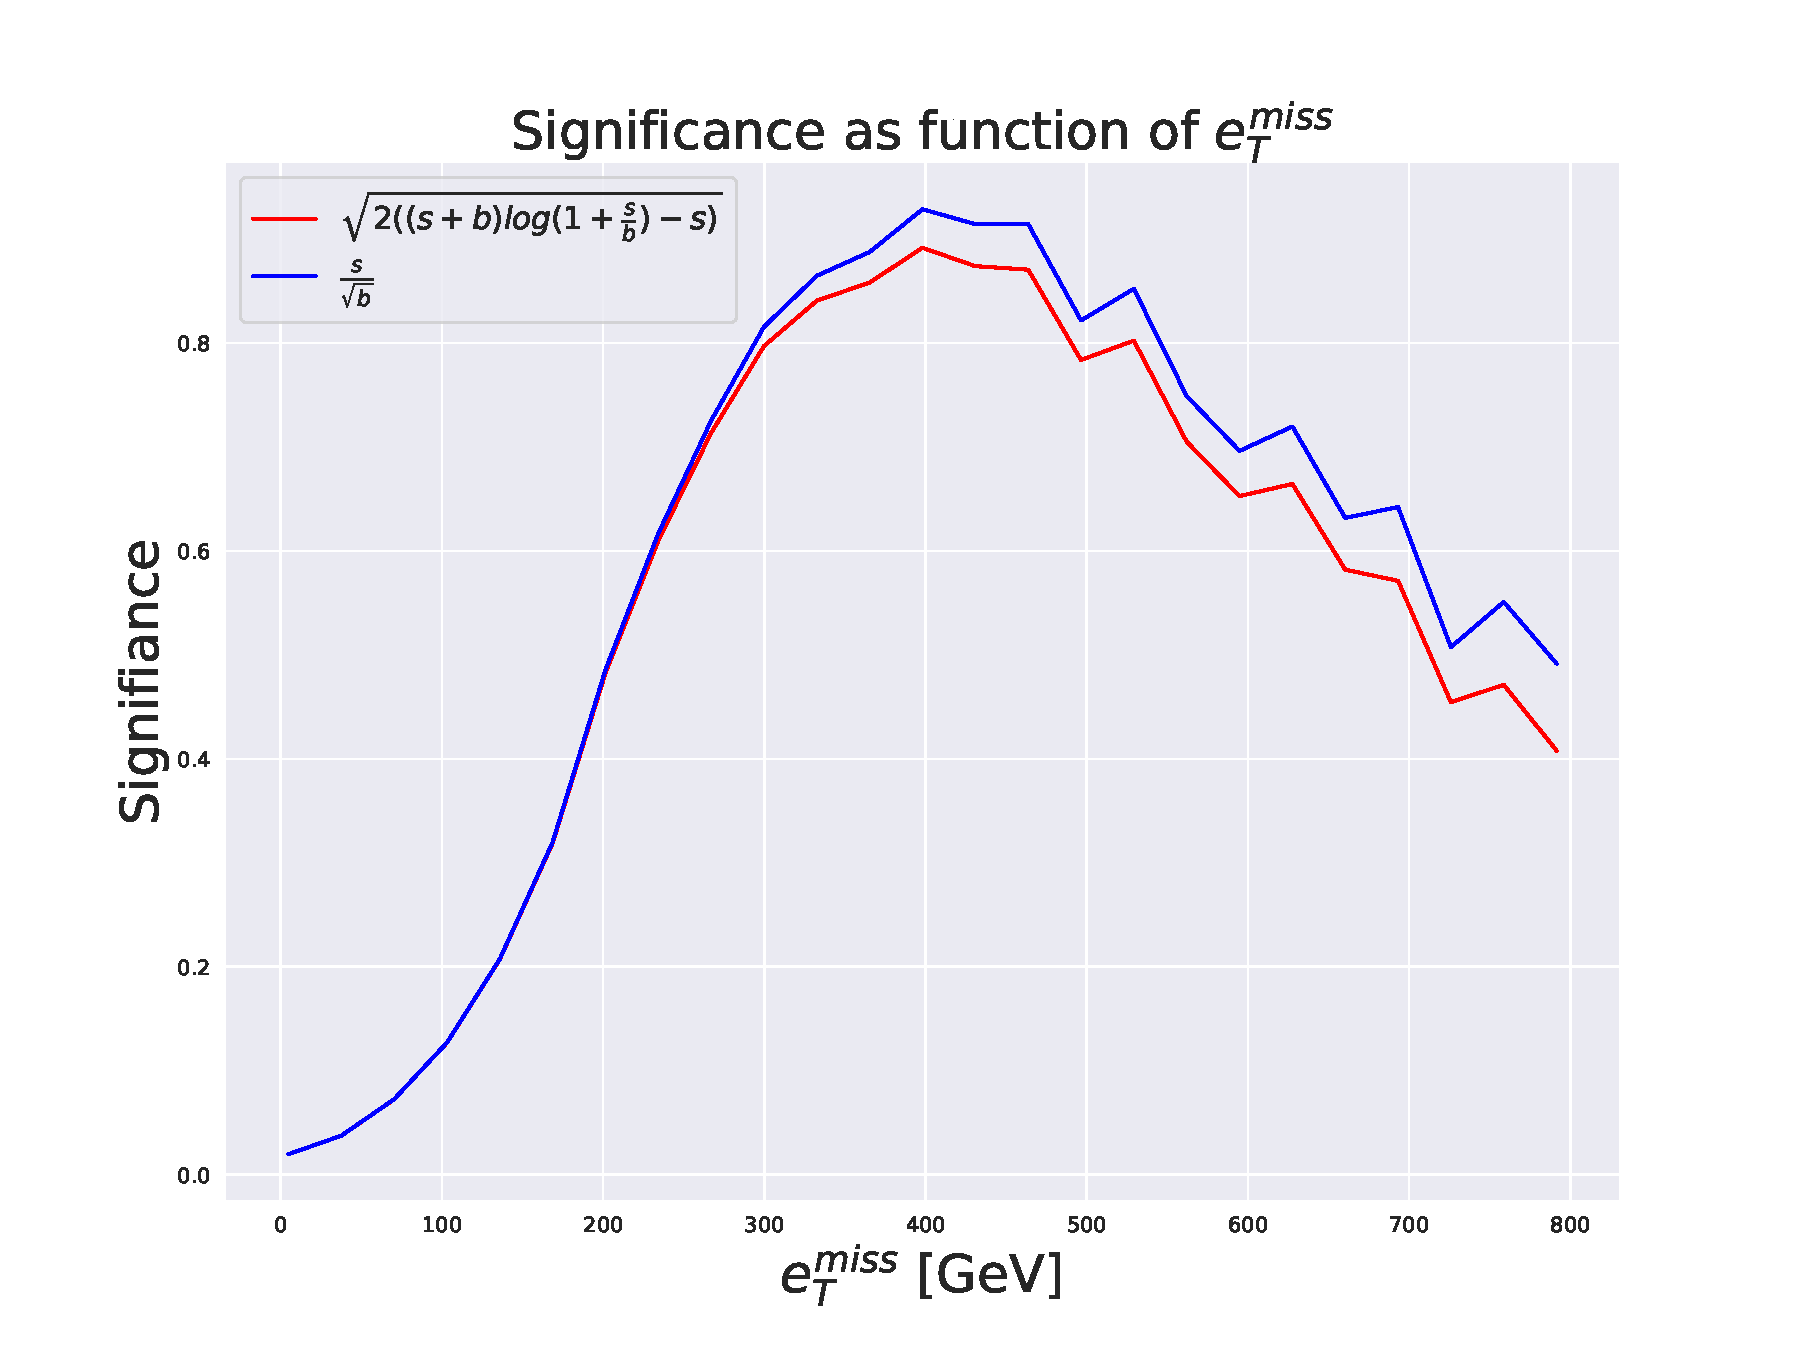
\includegraphics[width=\textwidth]{Figures/VAE_testing/small/2lep/significance_etmiss_450p0p0300_-0.4242401749818261.pdf}
        \caption{}
        \label{fig:VAE_2lep_small_signi_450_3}
    \end{subfigure}
    \hfill      
    \caption[2lep shallow network | $450p300$ | VAE | 3]{Reconstruction error, $e_T^{miss}$ signal region, $m_{lll}$ signal region and significance as function of 
    $e_T^{miss}$ for the deep regular autoencoder. Here the SUSY $450p300$ model is used.}
    \label{fig:VAE_2lep_small_rec_sig_signi_450_3}
\end{figure}


\begin{figure}[H]
    \centering
    \begin{subfigure}{.40\textwidth}
        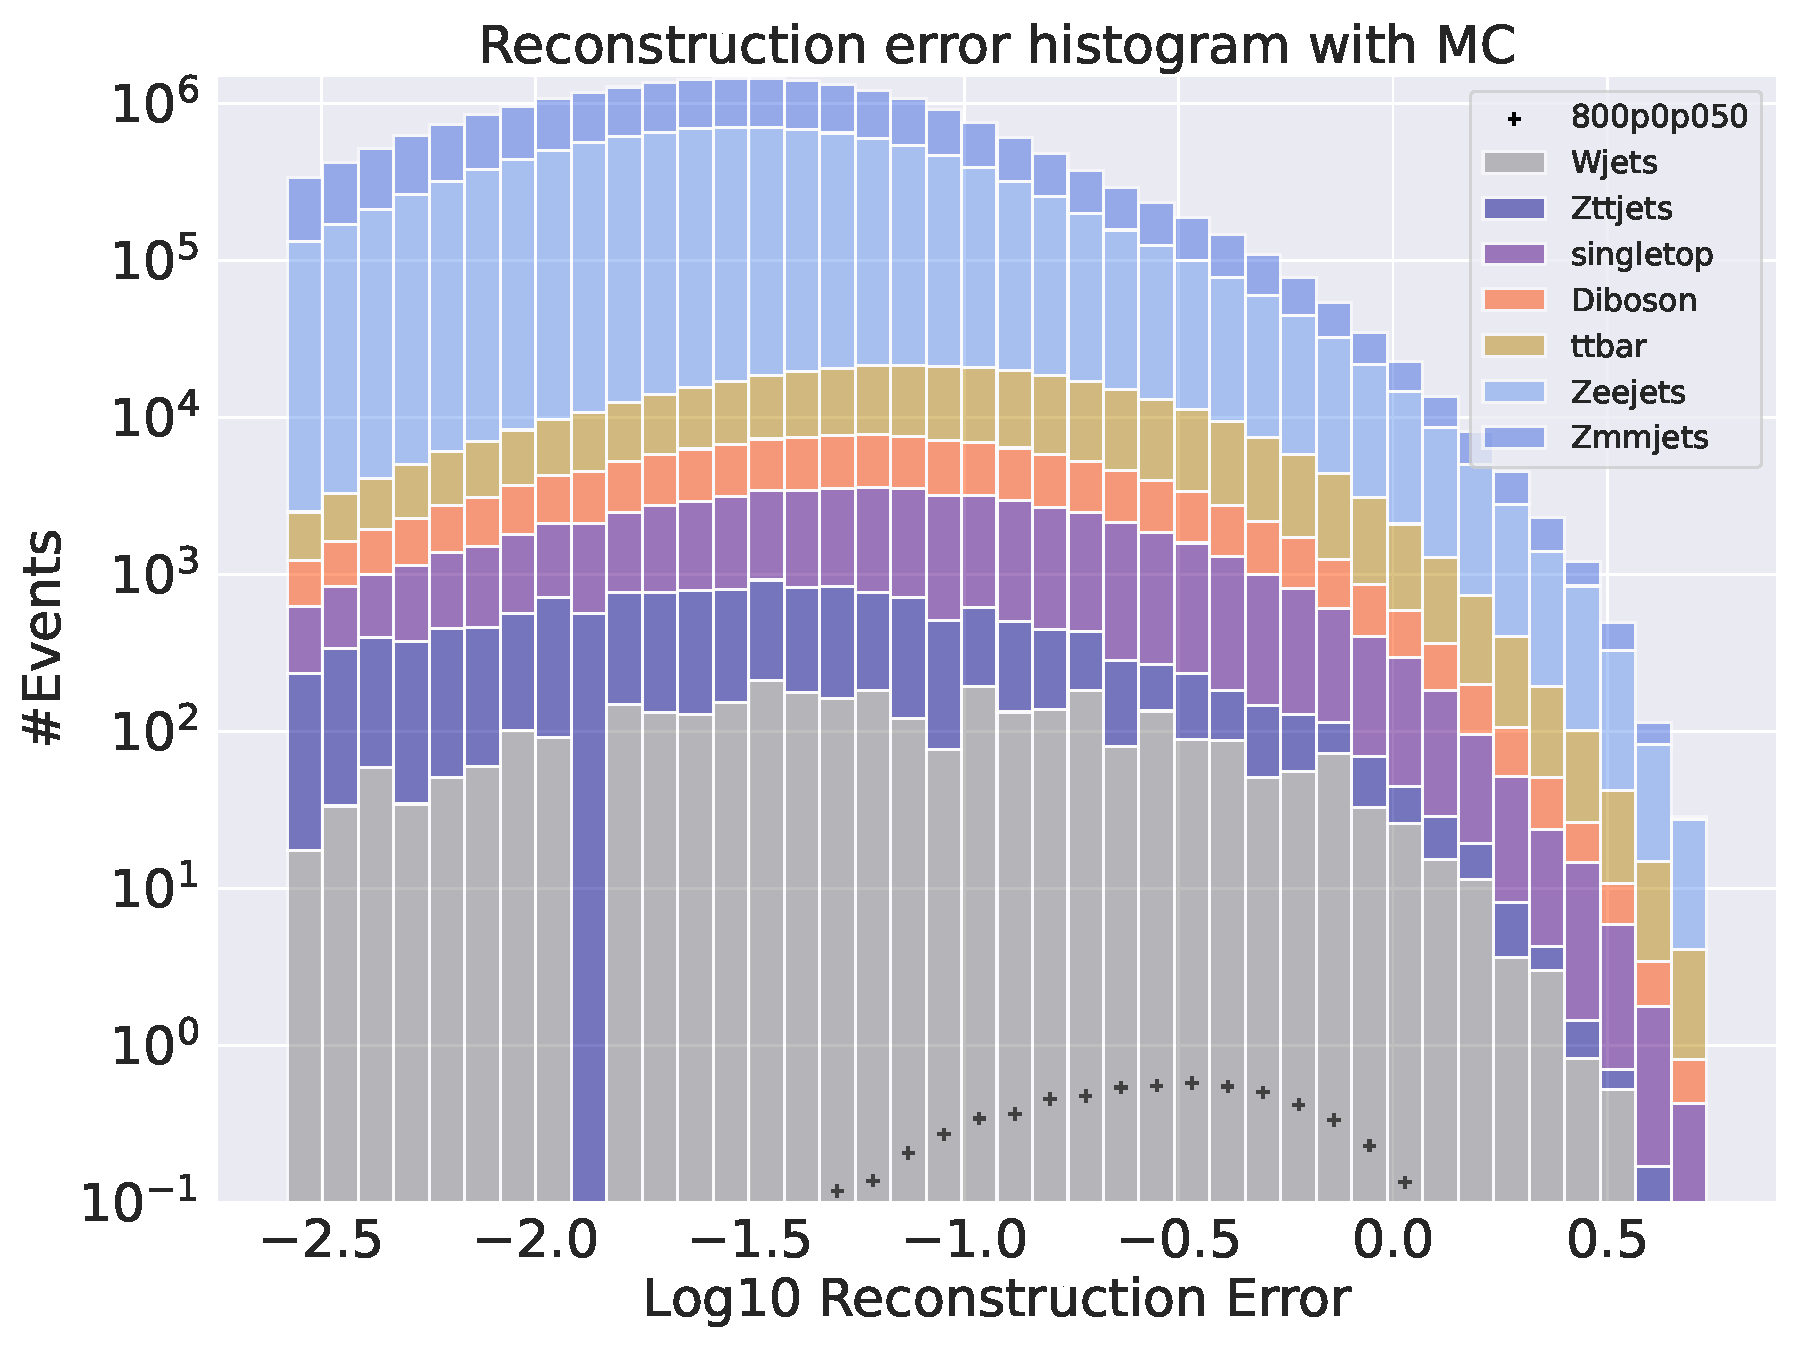
\includegraphics[width=\textwidth]{Figures/VAE_testing/big/2lep/b_data_recon_big_rm3_feats_sig_800p0p050_.pdf}
        \caption{ }
        \label{fig:VAE_2lep_big_800_3}
    \end{subfigure}
    \hfill
    \begin{subfigure}{.40\textwidth}
        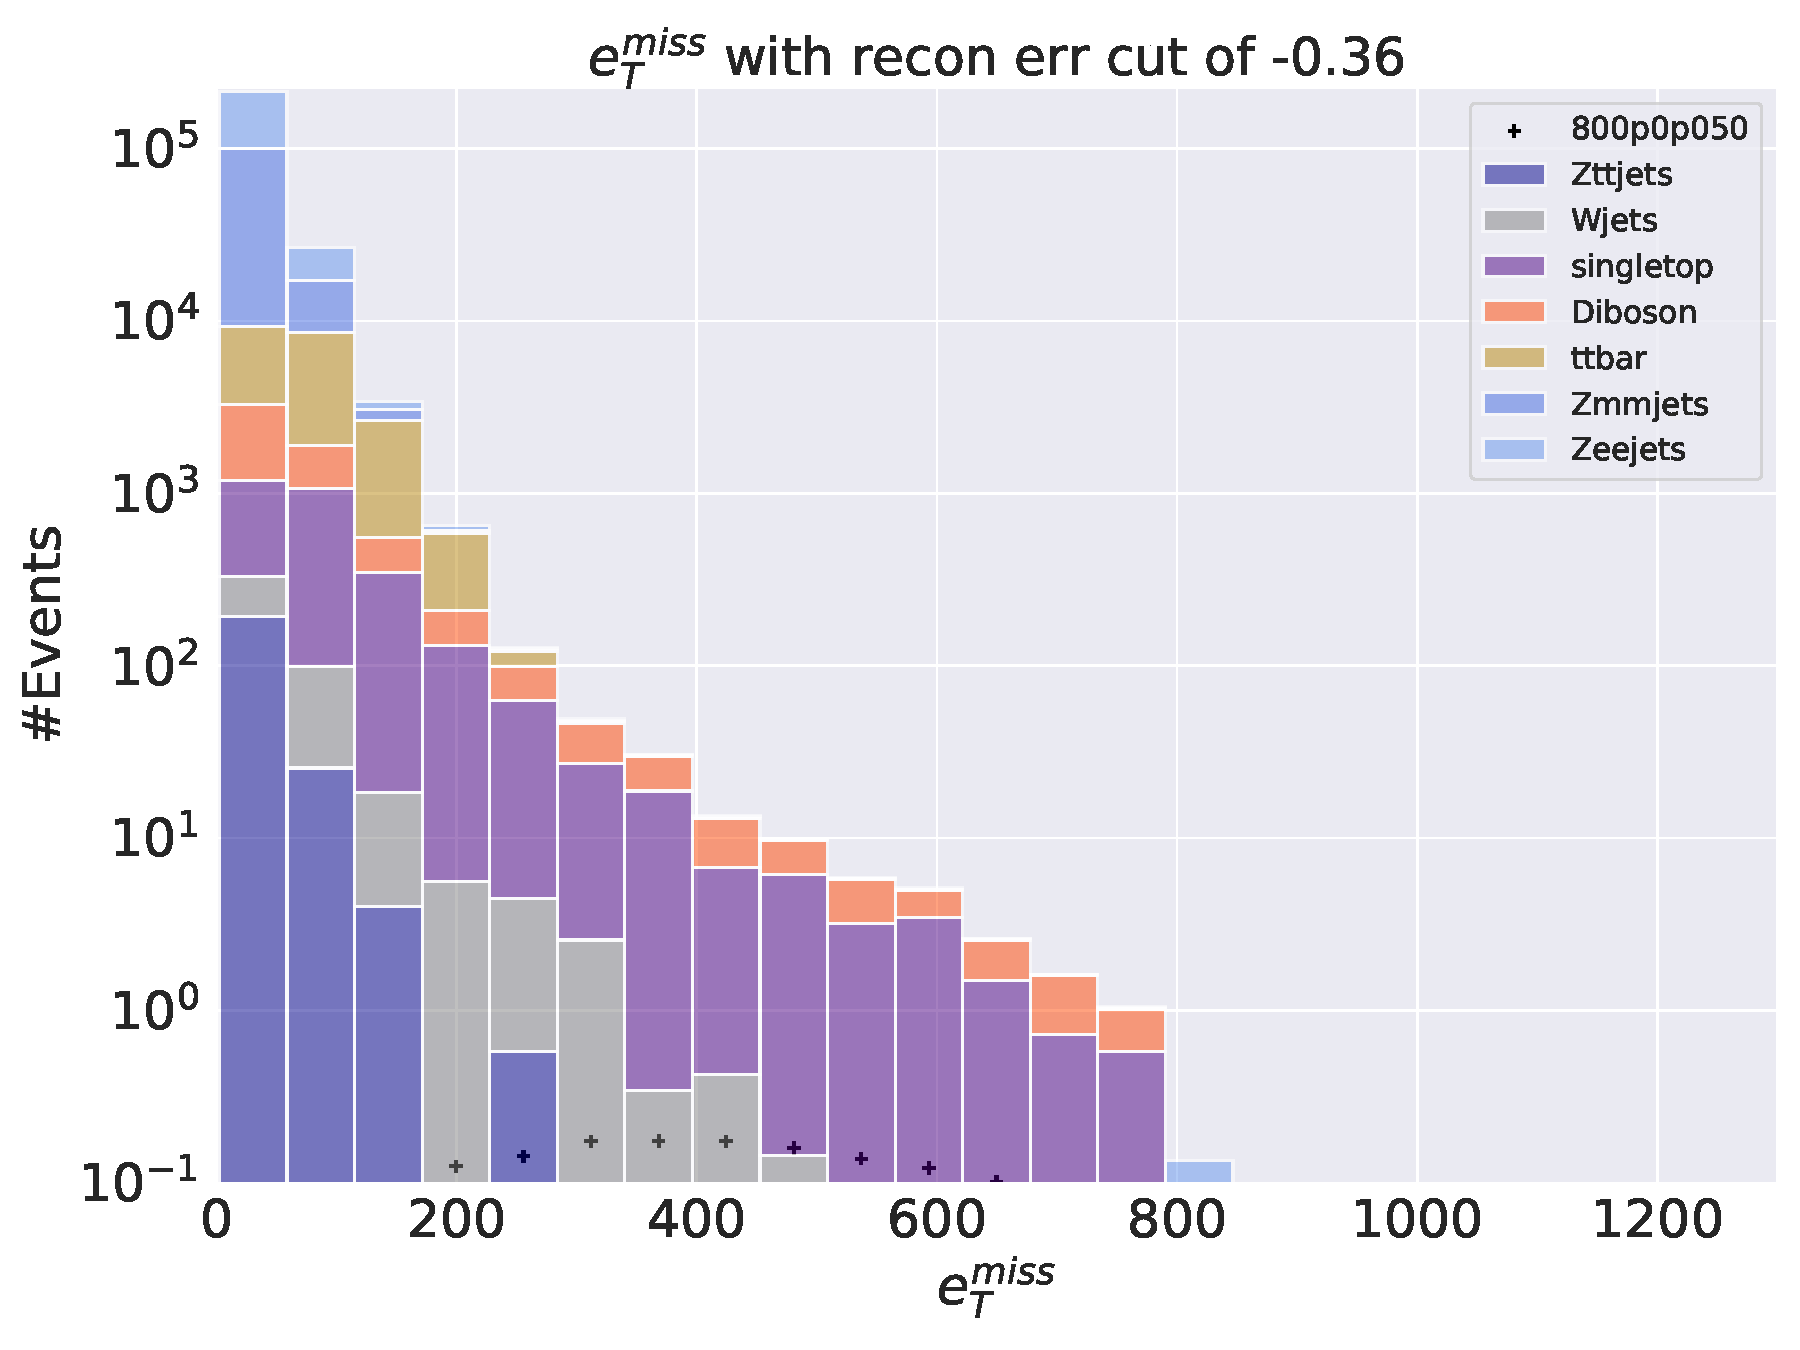
\includegraphics[width=\textwidth]{Figures/VAE_testing/big/2lep/b_data_recon_big_rm3_feats_sig_800p0p050_recon_errcut_-0.36.pdf}
        \caption{}
        \label{fig:VAE_2lep_big_etmiss_800_3}
    \end{subfigure}
    \hfill
      
    \begin{subfigure}{.40\textwidth}
        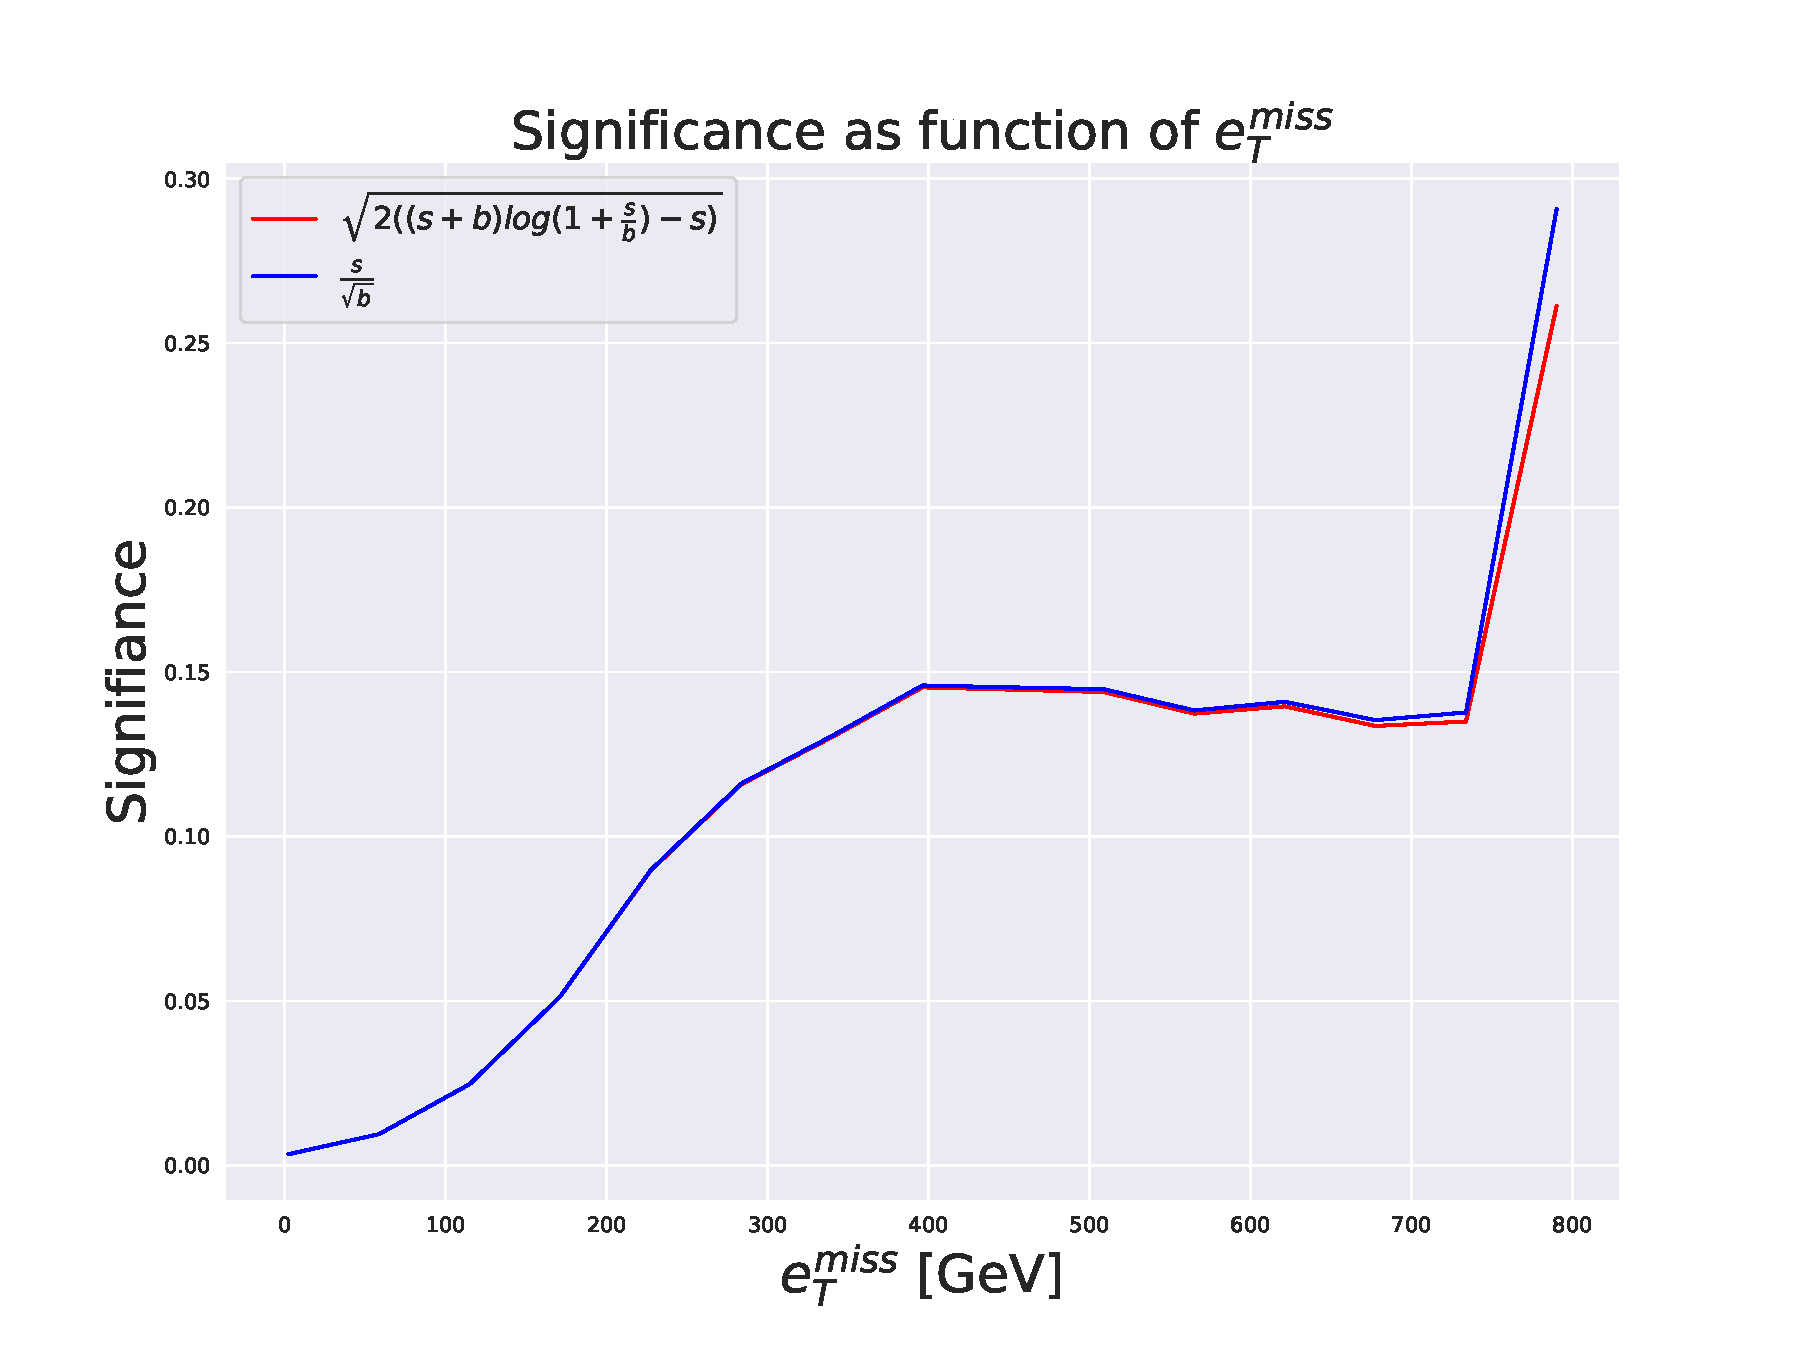
\includegraphics[width=\textwidth]{Figures/VAE_testing/big/2lep/significance_etmiss_800p0p050_-0.3616098672654746.pdf}
        \caption{}
        \label{fig:VAE_2lep_big_signi_800_3}
    \end{subfigure}
    \hfill      
    \caption[2lep deep network | $800p50$ | VAE | 3]{Reconstruction error, $e_T^{miss}$ signal region, $m_{lll}$ signal region and significance as function of 
    $e_T^{miss}$ for the deep regular autoencoder. Here the SUSY $800p50$ model is used.}
    \label{fig:VAE_2lep_big_rec_sig_signi_800_3}
\end{figure}

\begin{figure}[H]
    \centering
    \begin{subfigure}{.40\textwidth}
        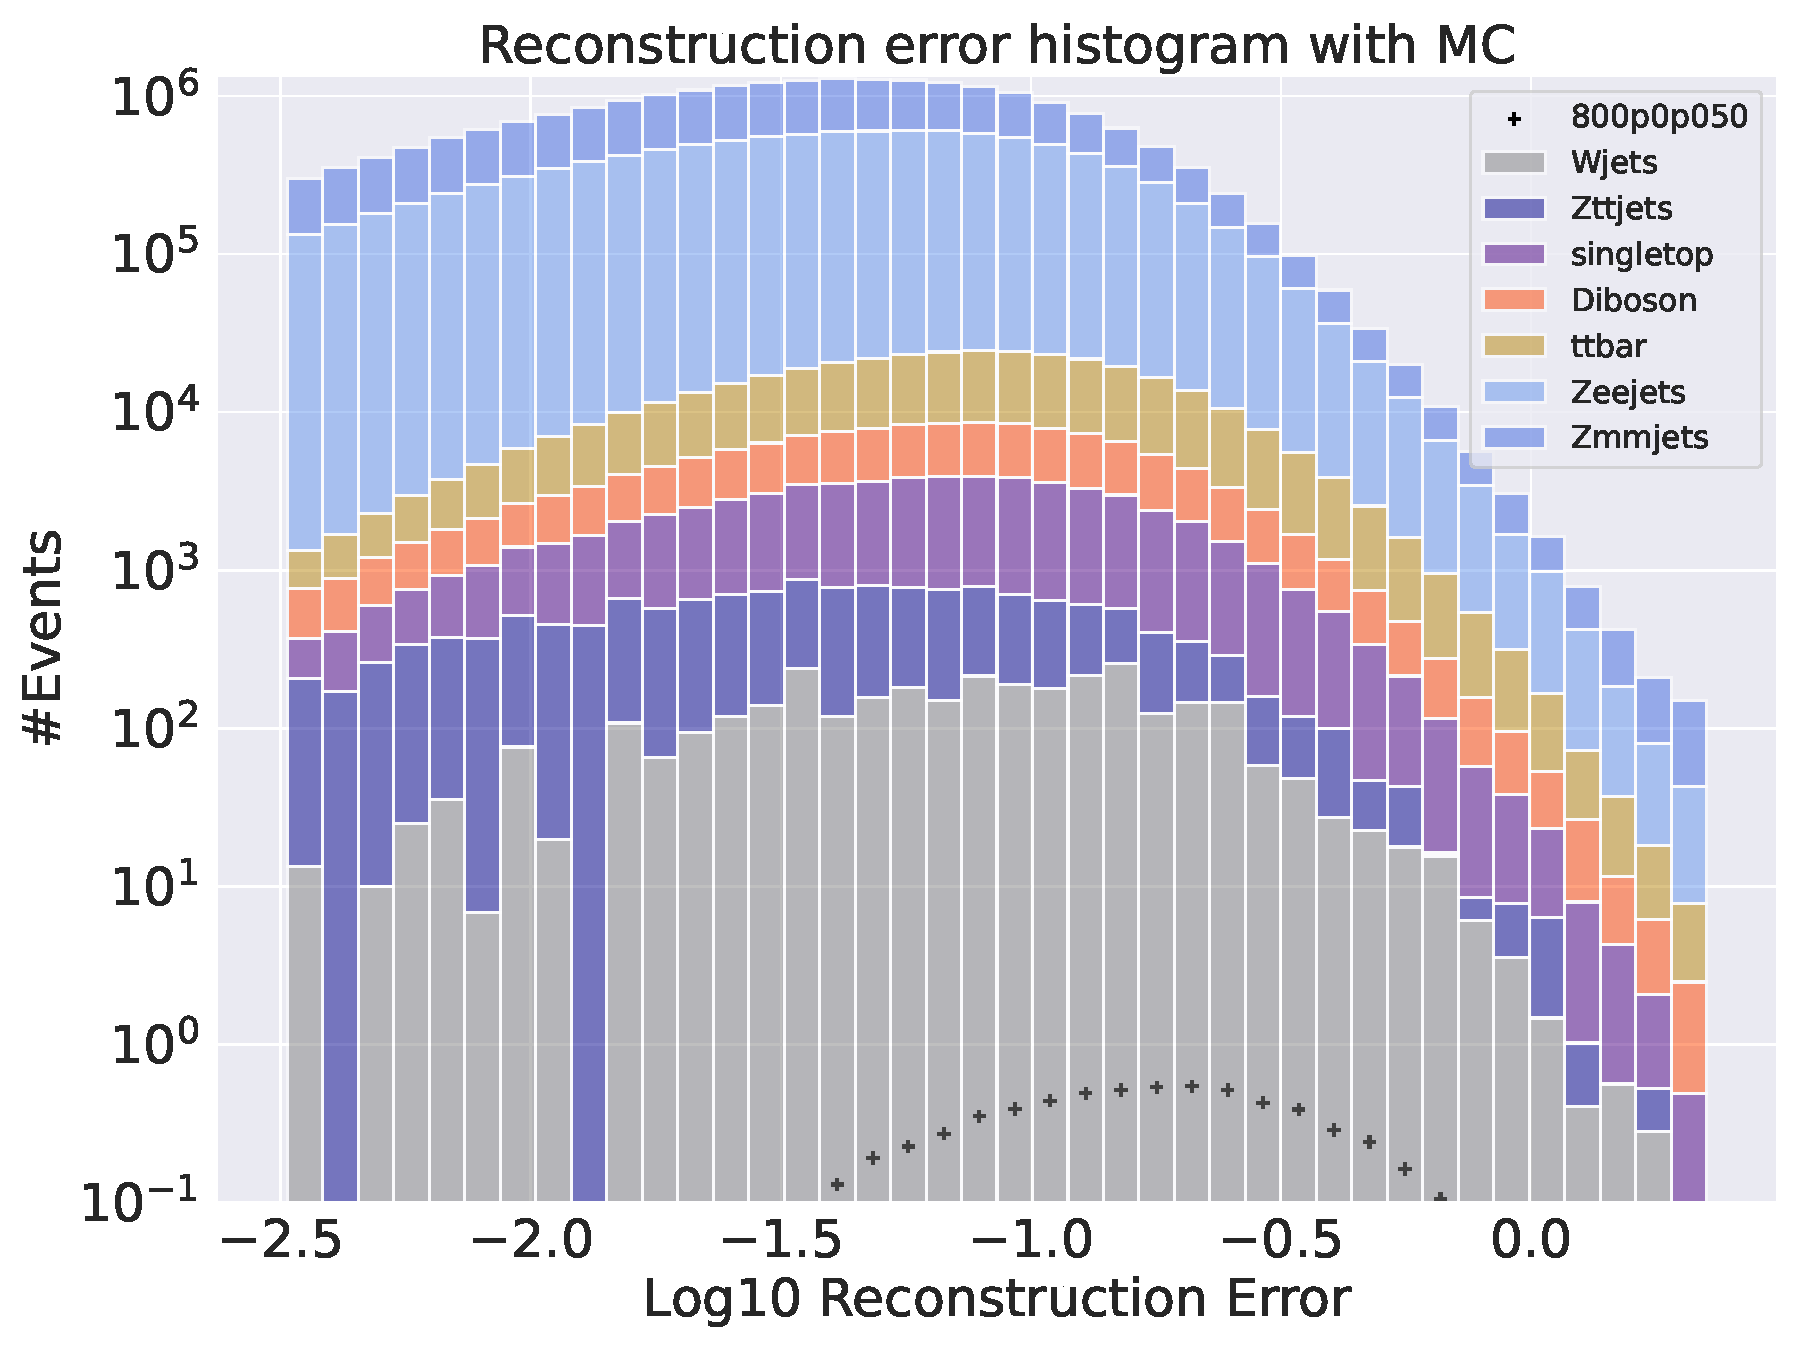
\includegraphics[width=\textwidth]{Figures/VAE_testing/small/2lep/b_data_recon_big_rm3_feats_sig_800p0p050_.pdf}
        \caption{ }
        \label{fig:VAE_2lep_small_800_3}
    \end{subfigure}
    \hfill
    \begin{subfigure}{.40\textwidth}
        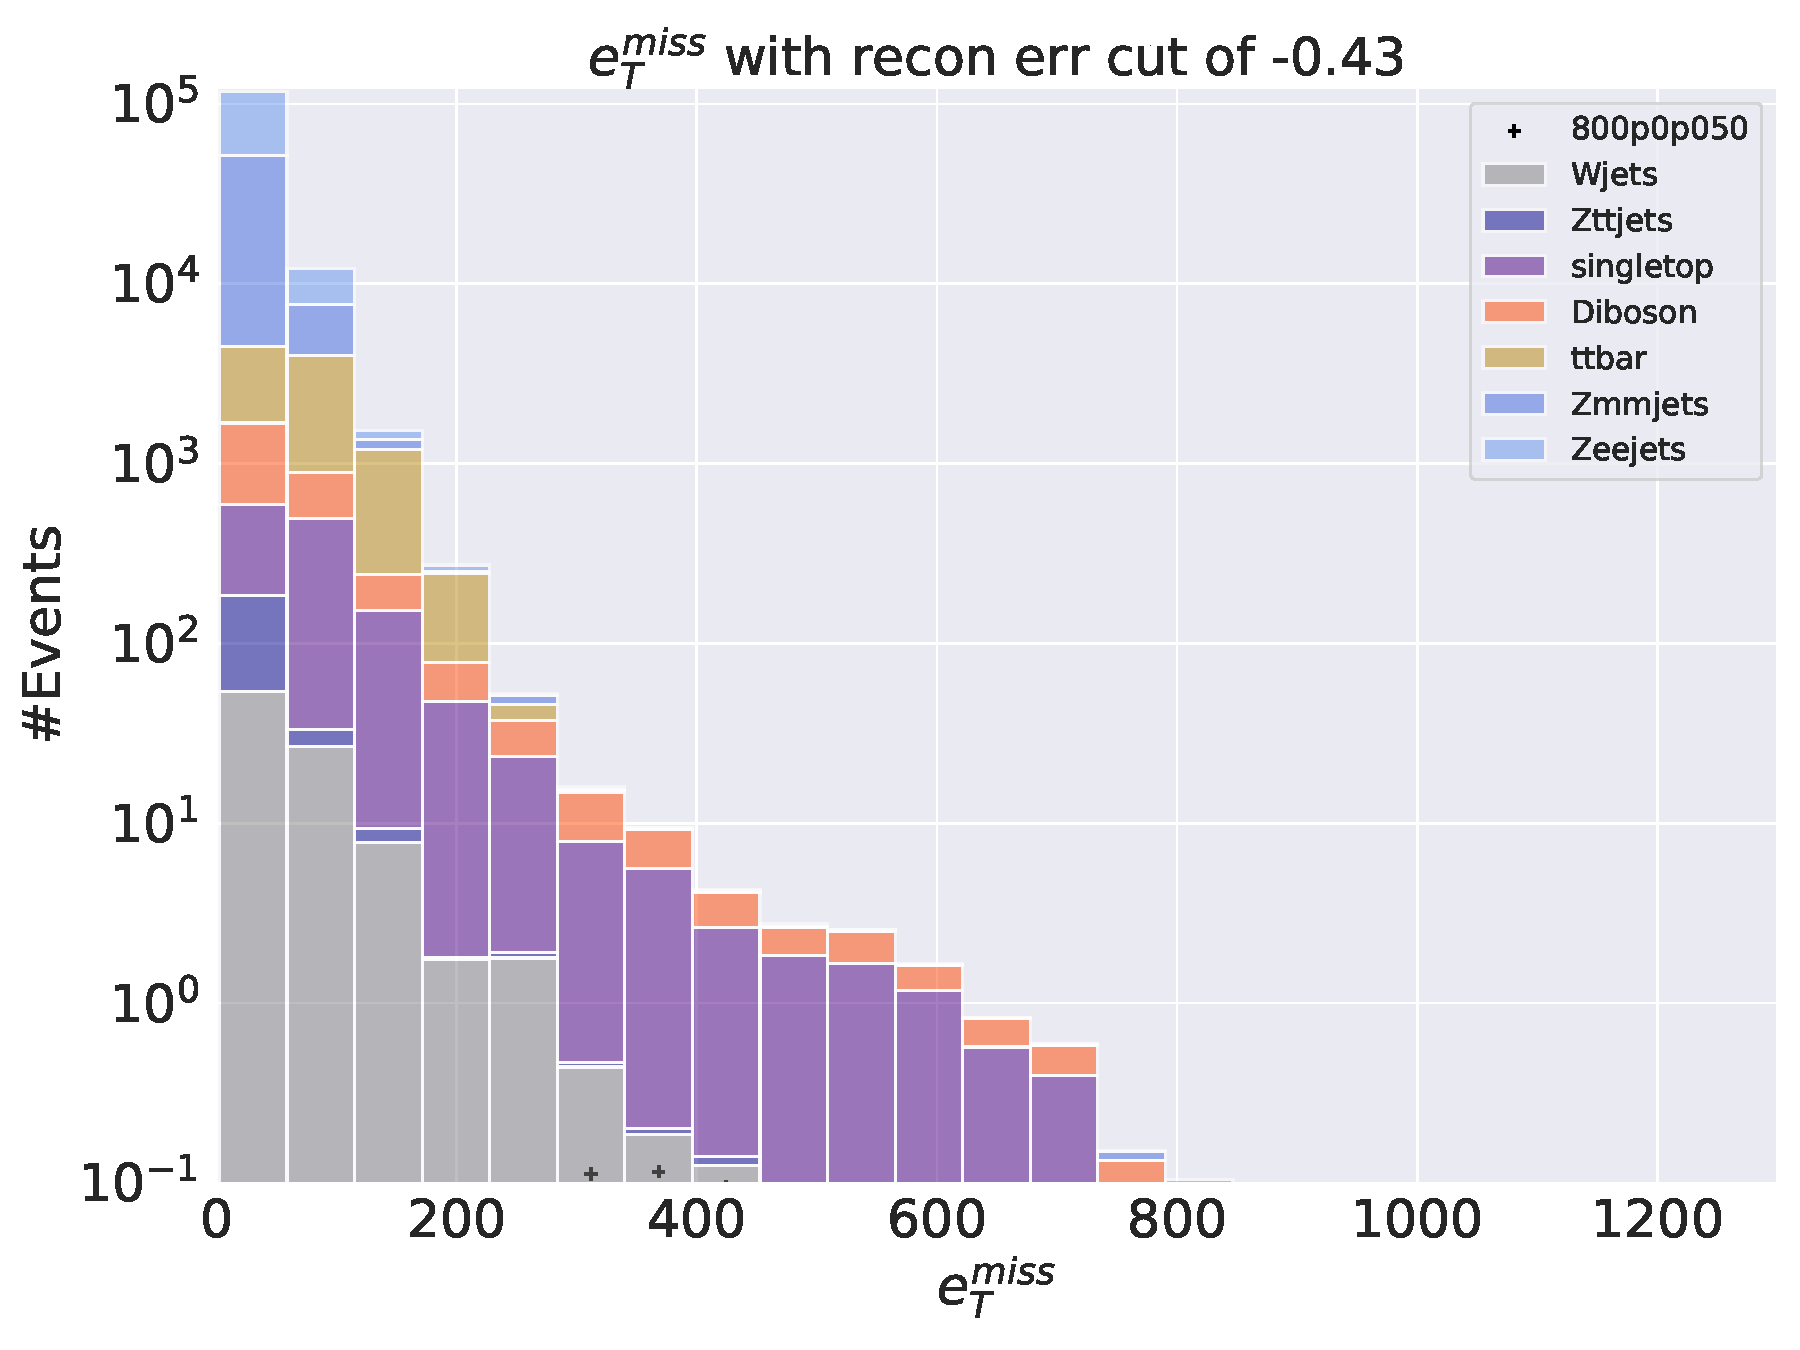
\includegraphics[width=\textwidth]{Figures/VAE_testing/small/2lep/b_data_recon_big_rm3_feats_sig_800p0p050_recon_errcut_-0.43.pdf}
        \caption{}
        \label{fig:VAE_2lep_small_etmiss_800_3}
    \end{subfigure}
    \hfill  
    \begin{subfigure}{.40\textwidth}
        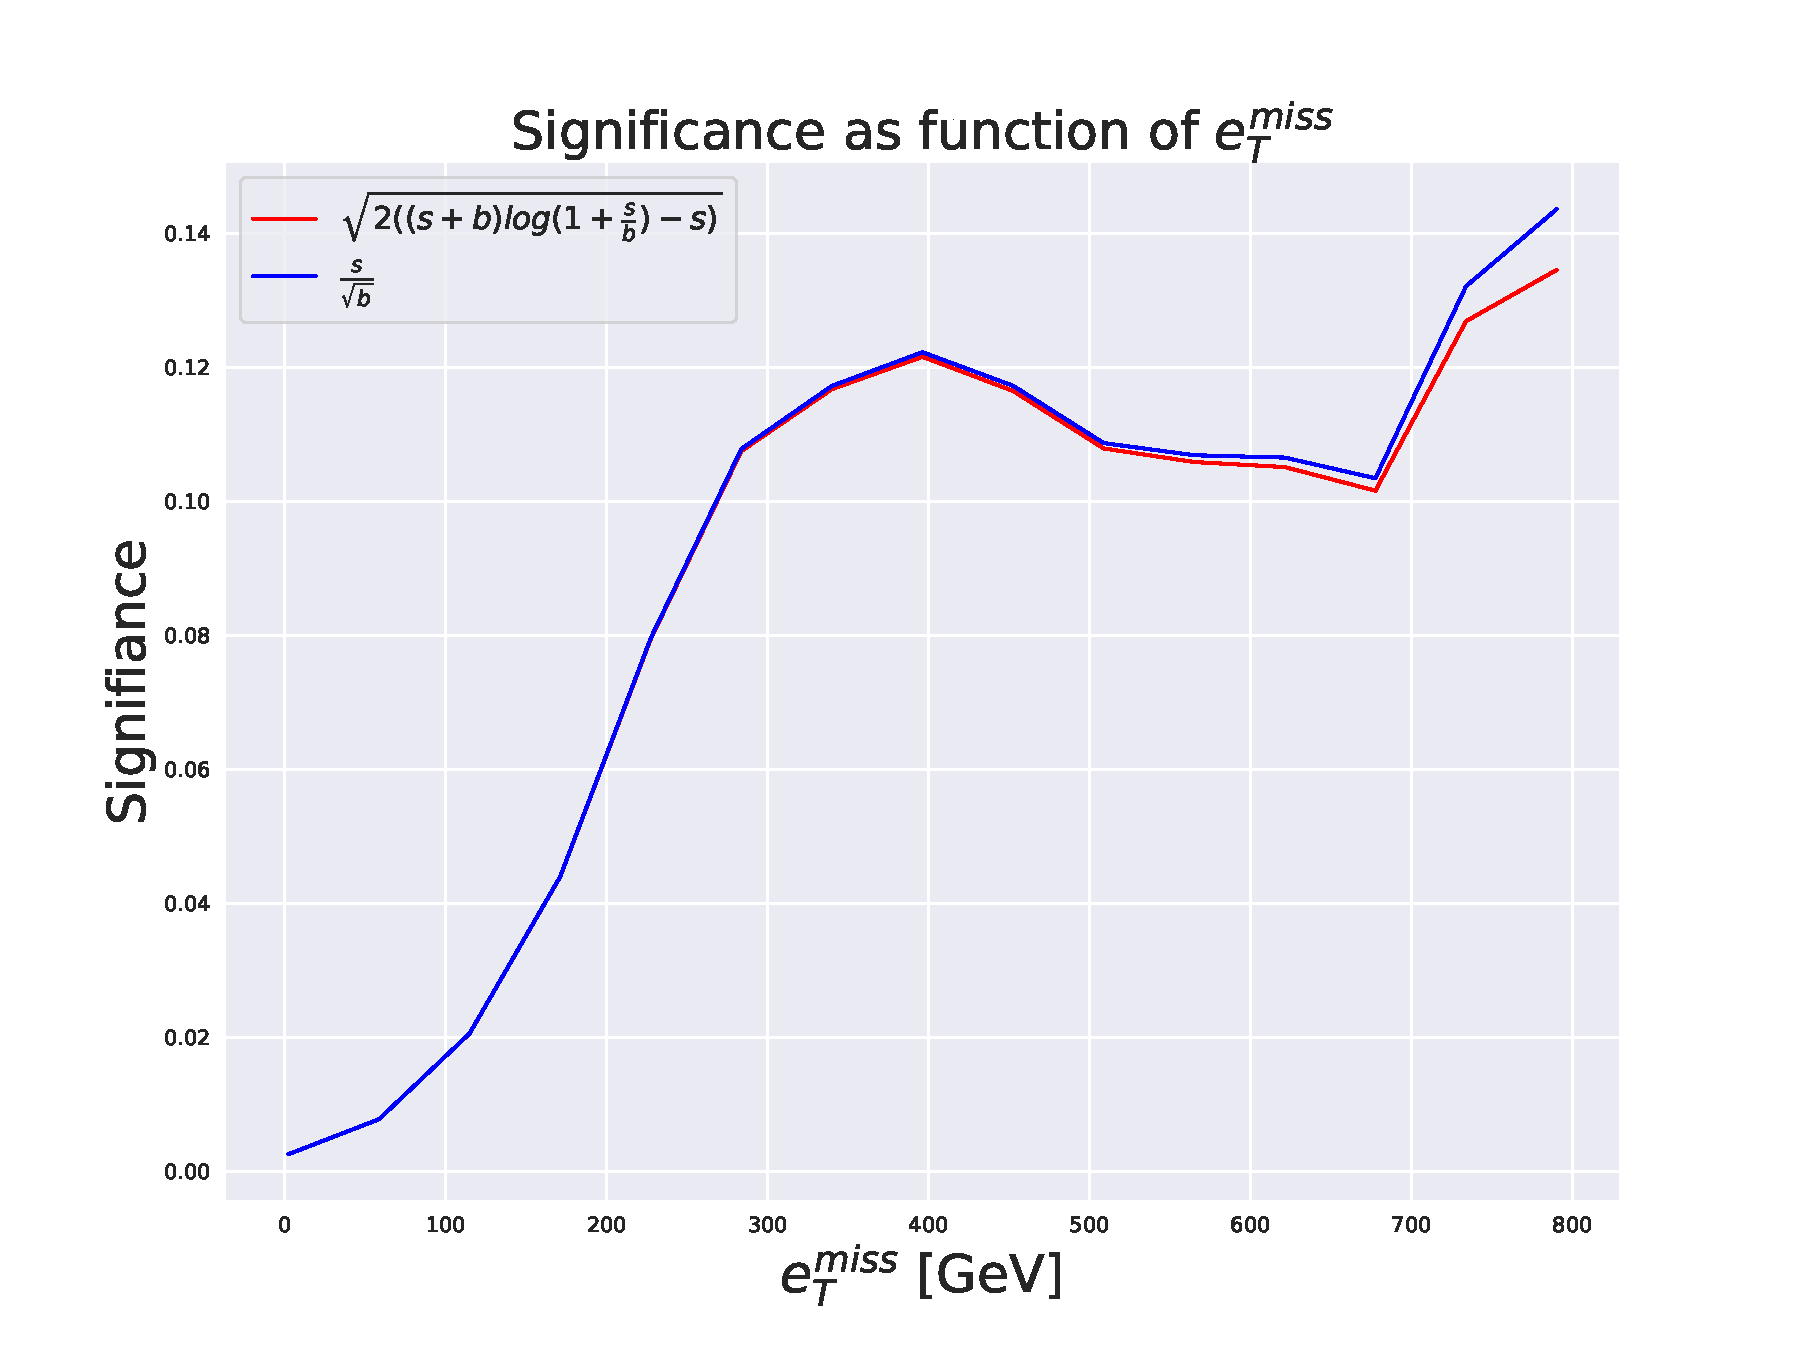
\includegraphics[width=\textwidth]{Figures/VAE_testing/small/2lep/significance_etmiss_800p0p050_-0.4271074800379211.pdf}
        \caption{}
        \label{fig:VAE_2lep_small_signi_800_3}
    \end{subfigure}
    \hfill      
    \caption[2lep shallow network | $800p50$ | VAE | 3]{Reconstruction error, $e_T^{miss}$ signal region, $m_{lll}$ signal region and significance as function of 
    $e_T^{miss}$ for the shallow regular autoencoder. Here the SUSY $800p50$ model is used.}
    \label{fig:VAE_2lep_small_rec_sig_signi_800_3}
\end{figure}


